\documentclass{article}

% packages
  % basic stuff for rendering math
  \usepackage[letterpaper, top=1in, bottom=1in, left=1in, right=1in]{geometry}
  \usepackage[utf8]{inputenc}
  \usepackage[english]{babel}
  \usepackage{amsmath} 
  \usepackage{amssymb}
  % \usepackage{amsthm}

  % extra math symbols and utilities
  \usepackage{mathtools}        % for extra stuff like \coloneqq
  \usepackage{mathrsfs}         % for extra stuff like \mathsrc{}
  \usepackage{centernot}        % for the centernot arrow 
  \usepackage{bm}               % for better boldsymbol/mathbf 
  \usepackage{bbm}
  \usepackage{enumitem}         % better control over enumerate, itemize
  \usepackage{hyperref}         % for hypertext linking
  \usepackage{fancyvrb}          % for better verbatim environments
  \usepackage{newverbs}         % for texttt{}
  \usepackage{xcolor}           % for colored text 
  \usepackage{listings}         % to include code
  \usepackage{lstautogobble}    % helper package for code
  \usepackage{parcolumns}       % for side by side columns for two column code
  \usepackage{algorithm}
  \usepackage{algpseudocode}

  % page layout
  \usepackage{fancyhdr}         % for headers and footers 
  \usepackage{lastpage}         % to include last page number in footer 
  \usepackage{parskip}          % for no indentation and space between paragraphs    
  \usepackage[T1]{fontenc}      % to include \textbackslash
  \usepackage{footnote}
  \usepackage{etoolbox}

  % for custom environments
  \usepackage{tcolorbox}        % for better colored boxes in custom environments
  \tcbuselibrary{breakable}     % to allow tcolorboxes to break across pages

  % figures
  \usepackage{pgfplots}
  \pgfplotsset{compat=1.18}
  \usepackage{float}            % for [H] figure placement
  \usepackage{tikz}
  \usepackage{tikz-cd}
  \usepackage{circuitikz}
  \usetikzlibrary{arrows.meta,backgrounds}
  \usetikzlibrary{circuits.logic.US}
  \usetikzlibrary{arrows}
  \usetikzlibrary{positioning}
  \usetikzlibrary{calc}
  \usepackage{graphicx}
  \usepackage{caption} 
  \usepackage{subcaption}
  \captionsetup{font=small}

  % for tabular stuff 
  \usepackage{dcolumn}

  \usepackage[nottoc]{tocbibind}
  \pdfsuppresswarningpagegroup=1
  \hfuzz=5.002pt                % ignore overfull hbox badness warnings below this limit

% New and replaced operators
  \DeclareMathOperator{\Tr}{Tr}
  \DeclareMathOperator{\Sym}{Sym}
  \DeclareMathOperator{\Span}{span}
  \DeclareMathOperator{\std}{std}
  \DeclareMathOperator{\Cov}{Cov}
  \DeclareMathOperator{\Var}{Var}
  \DeclareMathOperator{\Corr}{Corr}
  \DeclareMathOperator{\pos}{pos}
  \DeclareMathOperator*{\argmin}{\arg\!\min}
  \DeclareMathOperator*{\argmax}{\arg\!\max}
  \newcommand{\ket}[1]{\ensuremath{\left|#1\right\rangle}}
  \newcommand{\bra}[1]{\ensuremath{\left\langle#1\right|}}
  \newcommand{\braket}[2]{\langle #1 | #2 \rangle}
  \newcommand{\qed}{\hfill$\blacksquare$}     % I like QED squares to be black

% Custom Environments
  \newtcolorbox[auto counter, number within=section]{question}[1][]
  {
    colframe = orange!25,
    colback  = orange!10,
    coltitle = orange!20!black,  
    breakable, 
    title = \textbf{Question \thetcbcounter ~(#1)}
  }

  \newtcolorbox[auto counter, number within=section]{exercise}[1][]
  {
    colframe = teal!25,
    colback  = teal!10,
    coltitle = teal!20!black,  
    breakable, 
    title = \textbf{Exercise \thetcbcounter ~(#1)}
  }
  \newtcolorbox[auto counter, number within=section]{solution}[1][]
  {
    colframe = violet!25,
    colback  = violet!10,
    coltitle = violet!20!black,  
    breakable, 
    title = \textbf{Solution \thetcbcounter}
  }
  \newtcolorbox[auto counter, number within=section]{lemma}[1][]
  {
    colframe = red!25,
    colback  = red!10,
    coltitle = red!20!black,  
    breakable, 
    title = \textbf{Lemma \thetcbcounter ~(#1)}
  }
  \newtcolorbox[auto counter, number within=section]{theorem}[1][]
  {
    colframe = red!25,
    colback  = red!10,
    coltitle = red!20!black,  
    breakable, 
    title = \textbf{Theorem \thetcbcounter ~(#1)}
  } 
  \newtcolorbox[auto counter, number within=section]{proposition}[1][]
  {
    colframe = red!25,
    colback  = red!10,
    coltitle = red!20!black,  
    breakable, 
    title = \textbf{Proposition \thetcbcounter ~(#1)}
  } 
  \newtcolorbox[auto counter, number within=section]{corollary}[1][]
  {
    colframe = red!25,
    colback  = red!10,
    coltitle = red!20!black,  
    breakable, 
    title = \textbf{Corollary \thetcbcounter ~(#1)}
  } 
  \newtcolorbox[auto counter, number within=section]{proof}[1][]
  {
    colframe = orange!25,
    colback  = orange!10,
    coltitle = orange!20!black,  
    breakable, 
    title = \textbf{Proof. }
  } 
  \newtcolorbox[auto counter, number within=section]{definition}[1][]
  {
    colframe = yellow!25,
    colback  = yellow!10,
    coltitle = yellow!20!black,  
    breakable, 
    title = \textbf{Definition \thetcbcounter ~(#1)}
  } 
  \newtcolorbox[auto counter, number within=section]{example}[1][]
  {
    colframe = blue!25,
    colback  = blue!10,
    coltitle = blue!20!black,  
    breakable, 
    title = \textbf{Example \thetcbcounter ~(#1)}
  } 
  \newtcolorbox[auto counter, number within=section]{algo}[1][]
  {
    colframe = green!25,
    colback  = green!10,
    coltitle = green!20!black,  
    breakable, 
    title = \textbf{Algorithm \thetcbcounter ~(#1)}
  } 

  \BeforeBeginEnvironment{example}{\savenotes}
  \AfterEndEnvironment{example}{\spewnotes}
  \BeforeBeginEnvironment{lemma}{\savenotes}
  \AfterEndEnvironment{lemma}{\spewnotes}
  \BeforeBeginEnvironment{theorem}{\savenotes}
  \AfterEndEnvironment{theorem}{\spewnotes}
  \BeforeBeginEnvironment{corollary}{\savenotes}
  \AfterEndEnvironment{corollary}{\spewnotes}
  \BeforeBeginEnvironment{proposition}{\savenotes}
  \AfterEndEnvironment{proposition}{\spewnotes}
  \BeforeBeginEnvironment{definition}{\savenotes}
  \AfterEndEnvironment{definition}{\spewnotes}
  \BeforeBeginEnvironment{exercise}{\savenotes}
  \AfterEndEnvironment{exercise}{\spewnotes}
  \BeforeBeginEnvironment{proof}{\savenotes}
  \AfterEndEnvironment{proof}{\spewnotes}
  \BeforeBeginEnvironment{solution}{\savenotes}
  \AfterEndEnvironment{solution}{\spewnotes}
  \BeforeBeginEnvironment{question}{\savenotes}
  \AfterEndEnvironment{question}{\spewnotes}
  \BeforeBeginEnvironment{code}{\savenotes}
  \AfterEndEnvironment{code}{\spewnotes}
  \BeforeBeginEnvironment{algo}{\savenotes}
  \AfterEndEnvironment{algo}{\spewnotes}

  \definecolor{dkgreen}{rgb}{0,0.6,0}
  \definecolor{gray}{rgb}{0.5,0.5,0.5}
  \definecolor{mauve}{rgb}{0.58,0,0.82}
  \definecolor{darkblue}{rgb}{0,0,139}
  \definecolor{lightgray}{gray}{0.93}
  \renewcommand{\algorithmiccomment}[1]{\hfill$\triangleright$\textcolor{blue}{#1}}

  % default options for listings (for code)
  \lstset{
    autogobble,
    frame=ltbr,
    language=C,                           % the language of the code
    aboveskip=3mm,
    belowskip=3mm,
    showstringspaces=false,
    columns=fullflexible,
    keepspaces=true,
    basicstyle={\small\ttfamily},
    numbers=left,
    firstnumber=1,                        % start line number at 1
    numberstyle=\tiny\color{gray},
    keywordstyle=\color{blue},
    commentstyle=\color{dkgreen},
    stringstyle=\color{mauve},
    backgroundcolor=\color{lightgray}, 
    breaklines=true,                      % break lines
    breakatwhitespace=true,
    tabsize=3, 
    xleftmargin=2em, 
    framexleftmargin=1.5em, 
    stepnumber=1
  }

% Page style
  \pagestyle{fancy}
  \fancyhead[L]{Algorithms}
  \fancyhead[C]{Muchang Bahng}
  \fancyhead[R]{Spring 2024} 
  \fancyfoot[C]{\thepage / \pageref{LastPage}}
  \renewcommand{\footrulewidth}{0.4pt}          % the footer line should be 0.4pt wide
  \renewcommand{\thispagestyle}[1]{}  % needed to include headers in title page

\begin{document}

\title{Algorithms}
\author{Muchang Bahng}
\date{Spring 2024}

\maketitle
\tableofcontents
\pagebreak

\section{Complexity}

    A course on the study of algorithms. 

    \begin{definition}[Algorithm]
      An \textbf{algorithm} is a procedure for solving a mathematical problem in a \textit{finite} number of steps. It should be 
      \begin{enumerate}
        \item finite, 
        \item correct,
        \item efficient
      \end{enumerate}
    \end{definition}

    An algorithm, with respect to some inputs $\mathbf{n}$, will have a runtime that is some function $f$. We would like a formal way to analyze the asymptotic behavior between two functions. 

    \begin{definition}[Complexity]
      Given two positive functions $f, g$, 
      \begin{enumerate}
        \item $f = O(g)$ if $f/g$ is bounded.\footnote{Note that it is more accurate to write $f \in O(g)$, since we consider $O(g)$ a class of functions for which the property holds.} 
        \item $f = \Omega(g)$ if $g/f$ is bounded, i.e. $g = O(f)$. 
        \item $f = \Theta (g)$ if $f = O(g)$ and $g = O(f)$. 
      \end{enumerate}
    \end{definition}

    There are two notions of complexity here. We can compare $f$ and $g$ with respect to the \textit{value} $N$ of the input, or we can compare them with respect to the \textit{number of bits} $n$ in the input. While we mostly use the complexity w.r.t. the value, we should be aware for certain (especially low-level operations), the bit complexity is also important. 

    Let's do a quick comparison of various functions. Essentially, if we want to figure out the complexity of two positive functions $f, g$,\footnote{These will be positive since the runtime must be positive.} we can simply take the limit. 
    \begin{equation}
      \lim_{x \rightarrow +\infty} \frac{f(x)}{g(x)} = \begin{cases} 
        0 & \implies f = O(g) \\
        0 < x < +\infty & \implies f = \Theta(g) \\
        +\infty & \implies f = \Omega(g)
      \end{cases}
    \end{equation} 

    Most of the time, we will have to use L'Hopital's rule to derive these actual limits, but the general trend is 
    \begin{enumerate}
      \item $\log n$ is small  
      \item $\mathrm{poly}(n)$ grows faster
      \item $\exp(n)$ grows even faster 
      \item $n!$ even faster
      \item $n^n$ even faster
    \end{enumerate}

    \begin{theorem}[Properties]
      Some basic properties, which shows very similar properties to a vector space. 
      \begin{enumerate}
        \item Transitivity. 
        \begin{align}
          f = O(g), g = O(h) & \implies f = O(h) \\
          f = \Omega(g), g = \Omega(h) & \implies f = \Omega(h) \\
          f = \Theta(g), g = \Theta(h) & \implies f = \Theta(h) \\
        \end{align}

        \item Linearity.  
          \begin{align}
            f = O(h), g = O(h) & \implies f + g = O(h) \\
            f = \Omega(h), g = \Omega(h) & \implies f + g = \Omega(h) \\
            f = \Theta(h), g = \Theta(h) & \implies f + g = \Theta(h) \\
          \end{align}
      \end{enumerate}
    \end{theorem}

    \begin{example}
      Compare the following functions. 
      \begin{enumerate}
        \item $f(n) = \log_{10} (n), g(n) = \log_2 (n)$. Since they are different bases, we can write $f(n) = \log (n) / \log (10)$ and $g(n) = \log(n) / \log(2)$. They differ by a constant factor, so $f = \Theta(g)$. 

        \item $f(n) = (\log n)^{20}, g(n) = n$. We have 
        \begin{equation}
          \lim_{n \rightarrow \infty} \frac{(\log n)^20}{n} = \lim_{n \rightarrow \infty} \frac{20 \cdot (\log n)^{19} \cdot \frac{1}{n}}{1} = \ldots = \lim_{n \rightarrow \infty} \frac{20!}{n} = 0 \implies f = O(g)
        \end{equation}

        \item $f(n) = n^{100}, g(n) = 1.01^n$. We have 
          \begin{equation}
            \lim_{n \rightarrow \infty} \frac{n^{100}}{1.01^n} = \lim_{n \rightarrow \infty} \frac{100 n^{99}}{1.01^n \cdot \log (1.01)} =  \ldots = \lim_{n \rightarrow \infty} \frac{100!}{1.01^n \cdot (\log 1.01)^100} = 0 \implies f = O(g)
          \end{equation}
      \end{enumerate}
    \end{example}

    Let's do a slightly more nontrivial example. 

    \begin{example}
      Given the following algorithm, what is the runtime? 
      \begin{lstlisting}
        for i in range(1, n+1): 
          j = 1 
          while j <= i: 
            j = 2 * j
      \end{lstlisting}
      Now we can see that for each $i$, we will double up to $\log_2 (i)$ times. Therefore summing this all over $i$ is 
      \begin{equation}
        \sum_{i = 1}^n \log_2 (i) = \log_2 (n!) \leq \log_2 (n^n) = n \log_2 (n)
      \end{equation}
      and so we can see that the runtime is $O(n \log n)$. Other ways to do this is to just replace the summation with an integral.\footnote{Need more justification on why this is the case. Mentioned in lecture.} 
      \begin{equation}
        \int_1^n \log_2 (x) \,dx = x \log(x) - x \big|_1^n = n \log(n) - n + 1 = O(n \log n)
      \end{equation}
    \end{example}

\section{Brute Force Algorithms} 

  \subsection{Basic Arithmetic}

    In here, we use basic deductions from elementary algebra to give us a starting point at which we analyze fundamental arithmetic algorithms. 

    \begin{theorem}[Complexity of Addition]
      The complexity of addition of two $O(N)$ values with $n$ bits is
      \begin{enumerate}
        \item $O(n)$ bit complexity. 
        \item $O(\log N)$ complexity. 
        \item $O(1)$ memory complexity. 
      \end{enumerate}
      By the same logic, the complexity of subtraction is 
      \begin{enumerate}
        \item $O(n)$ bit complexity. 
        \item $O(\log N)$ complexity. 
        \item $O(1)$ memory complexity. 
      \end{enumerate}
    \end{theorem}
    \begin{proof}
      To see bit complexity, we are really taking each bit of each number and adding them together, plus a potential carry operation. Therefore, we are doing a bounded number of computations per bit, which is $O(1)$, but we must at least read through all of the bits, making this $O(\max\{n, m\})$. 
    \end{proof}

    \begin{theorem}[Complexity of Multiplication]
      The complexity of multiplication of two values $N, M$ with bits $n, m$ is 
      \begin{enumerate}
        \item $O(n^2)$ bit complexity.\footnote{It turns out we can do better, which we will learn later.} 
        \item $O((\log n)^2)$ complexity. 
        \item 
      \end{enumerate}
    \end{theorem}

    \begin{theorem}[Complexity of Division]
      The complexity of multiplication of two values $N, M$ with bits $n, m$ is 
      \begin{enumerate}
        \item $O(n^2)$ bit complexity. 
        \item 
      \end{enumerate}
    \end{theorem}

    \begin{theorem}[Complexity of Modulus]
      The complexity of multiplication of two values $N, M$ with bits $n, m$ is 
      \begin{enumerate}
        \item $O(n^2)$ bit complexity. 
        \item 
      \end{enumerate}
    \end{theorem}

    \begin{theorem}[Complexity of Exponentiation]
      The complexity of multiplication of two values $N, M$ with bits $n, m$ is 
      \begin{enumerate}
        \item $O(n^2)$ bit complexity. 
        \item 
      \end{enumerate}
    \end{theorem}

    \begin{theorem}[Complexity of Square Root]
      The complexity of multiplication of two values $N, M$ with bits $n, m$ is 
      \begin{enumerate}
        \item $O(n^2)$ bit complexity. 
        \item 
      \end{enumerate}
    \end{theorem}

    \begin{definition}[Factorial]
      
    \end{definition}
  
  \subsection{Lists} 

    \begin{definition}[Max and Min of List]
      
    \end{definition}

    \begin{definition}[Bubble Sort]

    \end{definition}

    \begin{definition}[Binary Search]
      
    \end{definition}

  \subsection{Stack, Queues, Heaps}

    A heap is sort of in between a sorted array and an unsorted array. 

  \subsection{Cryptography} 

    \begin{example}[GCD of Two Numbers]
      Take a look at the following algorithm. 
      \begin{lstlisting}
        def gcd(a, b): 
          if a == b: 
            return a
          elif a > b: 
            return gcd(a - b, b) 
          else: 
            return gcd(a, b - a)

        print(gcd(63, 210))
      \end{lstlisting}
    \end{example}

    \begin{definition}[Primality Testing]
      
    \end{definition}

    \begin{definition}[Integer Factorization]
      
    \end{definition}

  \subsection{Matrix Operations}

    \begin{definition}[Matrix Multiplication]
      
    \end{definition}

    \begin{definition}[Singular Value Decomposition]
      
    \end{definition}

    \begin{definition}[QR Decomposition]
      
    \end{definition}

    \begin{definition}[LU Decomposition]
      
    \end{definition}

    \begin{definition}[Matrix Inversion]
      
    \end{definition}

\section{Divide and Conquer} 

    \begin{definition}[Divide and Conquer Algorithms]
      The general idea is two steps: 
      \begin{enumerate}
        \item Divide an input into smaller instances of the same problem. The simplest form is merge sort. 
        \item Conquer/solve these smaller instances, which takes less time. 
        \item Merge/Combine the smaller solutions into the original, bigger solution. 
      \end{enumerate}
      This is usually recursive, but does not need to be. 
    \end{definition}

    It has its applications in the most elementary operations, in sorting and multiplication. To prove correctness, we use induction by proving the correctness of the base case and then the inductive step to show that there is an invariant. 
  
  \subsection{Recursive Algorithms and Recurrence Relation}

    I assume that the reader is familiar with recursive algorithms. Now to evaluate the runtime of a recursive algorithm, one must implicitly solve for the runtime of its recursive calls, and we can visualize it. 

    \begin{figure}[H]
      \centering 
      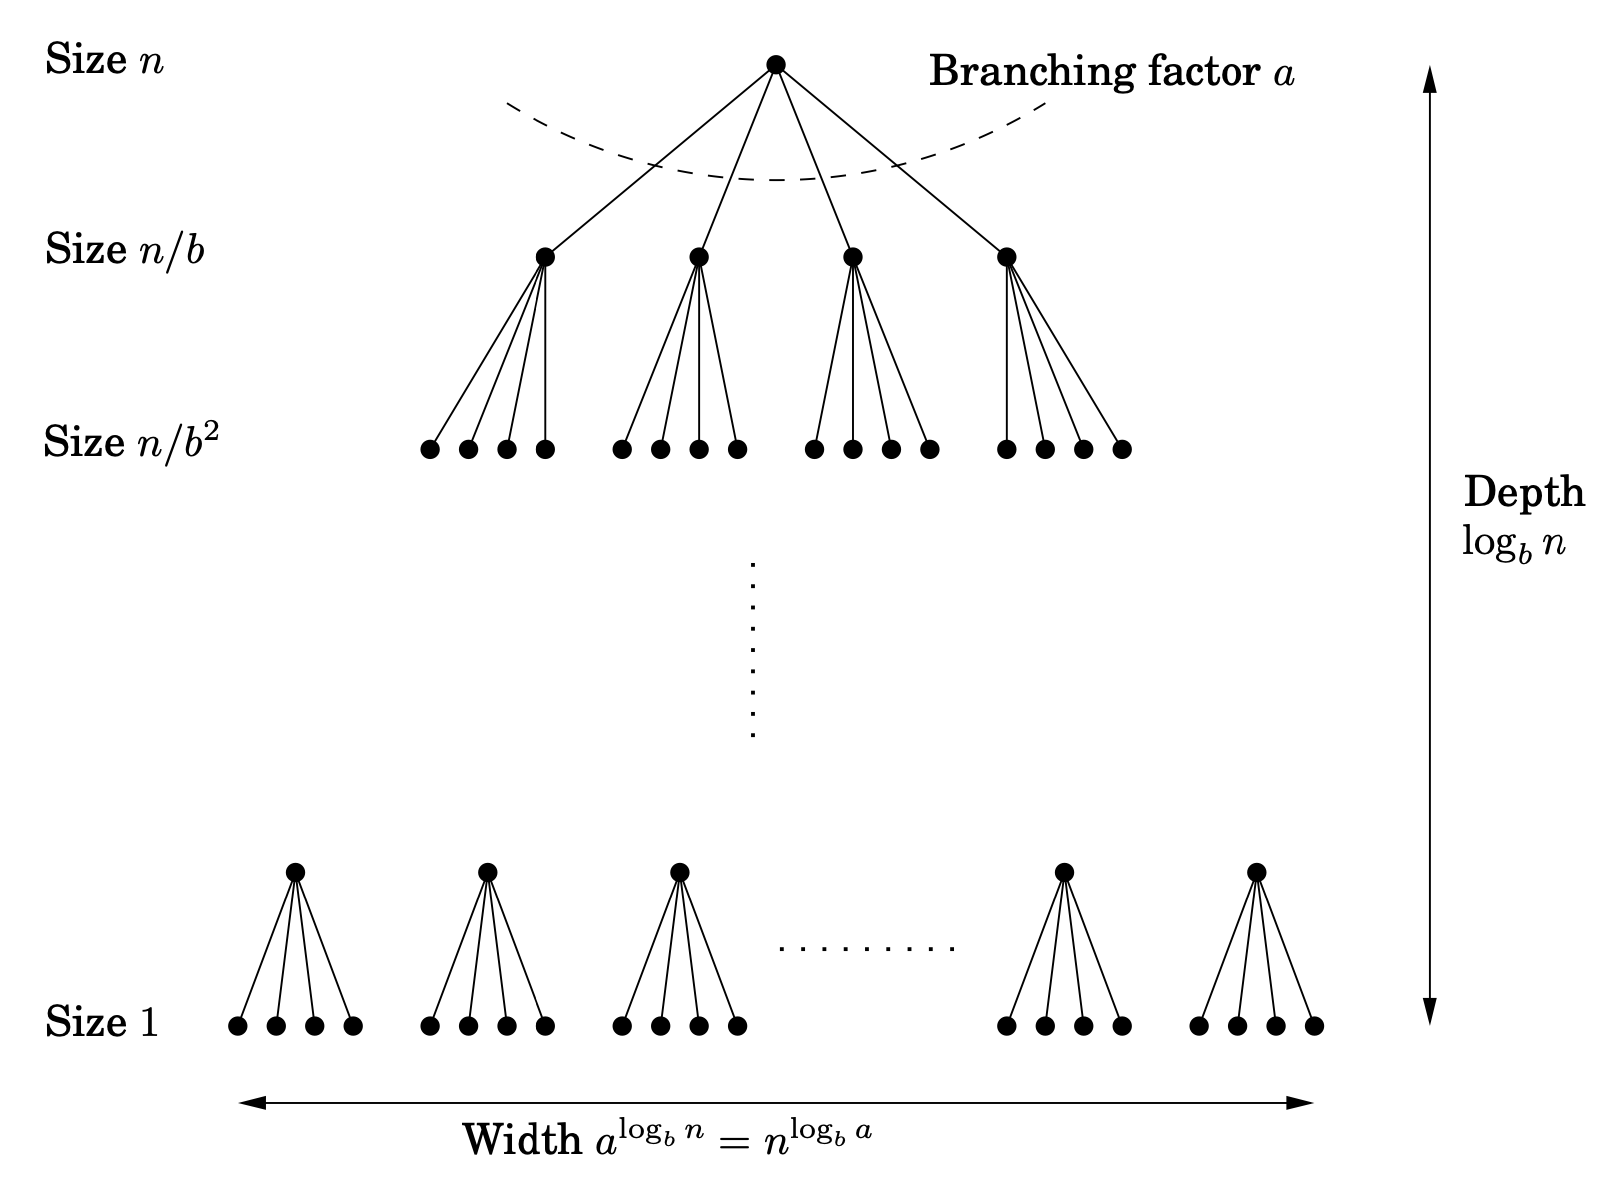
\includegraphics[scale=0.4]{img/branching.png}
      \caption{} 
      \label{fig:branching}
    \end{figure}

    An important theorem for divide-and-conquer algorithms is 

    \begin{theorem}[Master Theorem]
      Given a recurrence relation of form 
      \begin{equation}
        T(N) = a T(N/b) + O(N^c)
      \end{equation}
      then the following holds 
      \begin{align}
        a > b^c & \implies T(N) = O(N^{\log_b a}) \\
        a = b^c & \implies T(N) = O(N^c \log{N}) \\
        a < b^c & \implies T(N) = O(N^c) 
      \end{align}
    \end{theorem}
    \begin{proof}
      To intuit this, see that if $a > b^c$, then there arises a lot of subproblems, so our complexity is greater. If $a < b^c$, then we have few subproblems and can get a better runtime. If $a = b^c$, we get somewhere in between. To actually solve this, we can just unravel the recurrence to get the infinite series 
      \begin{align}
        T(N) & = a T(N/b) + O(N^c) \\
             & = a^2 T(N/b^2) +  N^c \bigg( \frac{a}{b^c} + 1 \bigg) \\
             & =  N^c \bigg( 1 + \frac{a}{b^c} + \frac{a^2}{b^{2c}} + \ldots \bigg)
      \end{align}
      So, if $a < b^c$, then even as $N \rightarrow \infty$, the sum is finite, so it is of order $O(N^c)$. If $a = b^c$, then the series is just $1 + \ldots + 1$, which scales on the order of $O(\log_2 {N})$. If $> 1$, then we have to calculate the last term, which contributes to our runtime and overpowers $c$.  
      
      Therefore, if $a$ is large, our algorithm will have an exponential number of subproblems and will be bottlenecked by the. 
    \end{proof}

  \subsection{Merge Sort and Counting Inversions}

    \begin{algo}[Merge Sort]
      Merge sort is the first instance. 
      \begin{algorithm}[H]
        \caption{Merge Sort}
        \label{alg:merge_sort}
        \begin{algorithmic}
          \Require{Array \texttt{nums}}
          \Function{MergeSort}{\texttt{nums}}
            \State \texttt{n = len(nums)}

            \If{\texttt{n < 2}} \Comment{base case}
              \State \Return{nums}
            \EndIf
            \State \texttt{mid = n // 2} 
            \State \texttt{left\_sorted = MergeSort(nums[:mid])} \Comment{Divide into left half}
            \State \texttt{right\_sorted = MergeSort(nums[mid:])} \Comment{Divide into right half}

            \State \texttt{res = [0] * n} 
            \State \texttt{i = j = k = 0} 
            \While{\texttt{k < n}} \Comment{Merge the sorted subarrays}
              \If{\texttt{j == len(right\_sorted) or left\_sorted[i] < right\_sorted[j]}}
                \State \texttt{res[k] = left\_sorted[i]} \Comment{We should add the next element from left array}
                \State \texttt{i += 1} \Comment{if it is smaller or if right array is filled already}
              \Else 
                \State \texttt{res[k] = right\_sorted[j]}
                \State \texttt{j += 1}
              \EndIf 
              \State \texttt{k += 1}
            \EndWhile

            \State \Return{\texttt{res}}
          \EndFunction
        \end{algorithmic}
      \end{algorithm}
      The recurrence relation for the runtime is as follows. Let $T(n)$ represent the worst-case runtime of \texttt{MergeSort} of size $n$. Then, we have 
      \begin{equation}
        T(n) = 2 \cdot T(n/2) + O(n)
      \end{equation}
      Consisting of two recursive calls with input size $n/2$ and then the merge step which is $O(n)$. But if we take a look at this, we have 
      \begin{align}
        T(n) & = 2 \cdot T(n/2) + O(n) \\
             & = 2 \cdot \big( 2 \cdot T(n/4) + O(n/2)) + O(n) \\
             & = 4 \cdot T(n/4) + O(n) + O(n) 
      \end{align}
      and the number of times $O(n)$ is added up is $\log{n}$, meaning that this recurrence relation turns into $O(n \log{n})$. 
    \end{algo}

    \begin{definition}[Inversions]
      Given two lists of ranked items, say 
      \begin{align}
        \text{Alice}: & a > b > c > d > e \\
        \text{Bob}: & b > d > a > e > c
      \end{align}
      We want to measure the dissimilarity between two rankings by counting the number of \textit{inversions}, which are pairs of items for which open persons orders the opposite of the other (e.g. $a, b$ for above).\footnote{Also known as Kendall-Tau distance in statistics.} So how many inversions are there? We can do this in $\Theta(n^2)$ by explicitly looking at all $n$ pairs. Without loss of generality, we can assume that the first list is sorted simply by bijectively relabeling these elements for both lists. Therefore, the set of inversions is defined to be 
      \begin{equation}
        \{(i, j) \text{ s.t. } i < j \text{ and } \texttt{A[i] > A[j]}\}
      \end{equation}
    \end{definition}

    \begin{algo}[Counting Inversions]
      The idea is very similar. By assuming that the first list is sorted, we can simply count the number of inversions in a single list $A$.  
      \begin{lstlisting}
        A = 5 6 1 3 4 8 2 7
      \end{lstlisting}
      \begin{enumerate}
        \item In the divide step, we count all inversions in $A_l, A_r$, which are the left and right sides of $A$, \textit{and} we sort $A_l, A_r$ to add additional structure.  
          \begin{lstlisting}
            1 3 5 6 | 2 4 7 8
          \end{lstlisting}
        \item In the conquer step, we merge them linearly but every time we add an element from $A_r$ into our result, this reveals that there are $k$ additional inversions added where $k$ is the number of elements left in $A_l$ to add.  
      \end{enumerate}
      \begin{algorithm}[H]
        \caption{Counting Inversions}
        \label{alg:inversions}
        \begin{algorithmic}
          \Require{Array \texttt{nums}}
          \Function{Inversions}{\texttt{nums}}
            \State \texttt{n = len(nums)}

            \If{\texttt{n < 2}} \Comment{base case}
              \State \Return{nums}
            \EndIf
            \State \texttt{mid = n // 2} 
            \State \texttt{left\_sorted, left\_invs = Inversions(nums[:mid])} \Comment{Divide into left half}
            \State \texttt{right\_sorted, right\_invs = Inversions(nums[mid:])} \Comment{Divide into right half}

            \State \texttt{res = [0] * n} 
            \State \texttt{i = j = k = 0} \Comment{left, right, and combined index}
            \State \texttt{inv = 0} \Comment{number of inversions}
            \While{\texttt{k < n}} \Comment{Merge the sorted subarrays}
              \If{\texttt{j == len(right\_sorted) or left\_sorted[i] < right\_sorted[j]}}
                \State \texttt{res[k] = left\_sorted[i]} \Comment{We should add the next element from left array}
                \State \texttt{invs += len(left\_sorted - i)} \Comment{Increment inversions by \# of elems in left array}
                \State \texttt{i += 1} \Comment{if it is smaller or if right array is filled already}
              \Else 
                \State \texttt{res[k] = right\_sorted[j]}
                \State \texttt{j += 1}
              \EndIf 
              \State \texttt{k += 1}
            \EndWhile

            \State \Return{\texttt{res, inv + left\_invs + right\_invs}}
          \EndFunction
        \end{algorithmic}
      \end{algorithm}
      The recursion relation is still 
      \begin{equation}
        T(n) = 2 \cdot T(n/2) + O(1) + O(n) \implies O(n \log{n})
      \end{equation}
    \end{algo}

  \subsection{Selection and Quick Sort} 
  
    The next problem is a generalization of finding the median of an array, which we present can be done in $O(n)$ time \textit{on average}. It turns out that that this idea of choosing a pivot and then dividing and conquering happens often in general selection and sort algorithms.    

    \begin{algo}[Select kth Largest Element from Unsorted Array]

      \begin{algorithm}[H]
        \caption{Find Kth Largest Element}
        \label{alg:kth_largest}
        \begin{algorithmic}
          \Require{Array of numbers nums, integer k where 1 <= k <= length(nums)}
          \State
          \Function{FindKthLargest}{nums, k}
              \If{length(nums) = 1} \Comment{Base case: if array has only one element}
                  \State \Return nums[0]
              \EndIf
              
              \State pivot $\gets$ $\lfloor$length(nums)/2$\rfloor$ \Comment{Select middle element as pivot}
              \State left $\gets$ [ ] \Comment{Unsorted array for elements smaller than pivot}
              \State right $\gets$ [ ] \Comment{Unsorted array for elements larger than pivot}
              \State n\_pivots $\gets$ 0 \Comment{Count of elements equal to pivot}
              
              \For{each n in nums} \Comment{Start filling in the arrays}
                  \If{n = nums[pivot]}
                      \State n\_pivots $\gets$ n\_pivots + 1
                  \ElsIf{n $\leq$ nums[pivot]}
                      \State left.append(n)
                  \Else
                      \State right.append(n)
                  \EndIf
              \EndFor
              
              \If{length(right) $\leq$ k - 1 \textbf{and} length(left) $\leq$ length(nums) - k}
                \State \Return nums[pivot] \Comment{Found the $k$th element which was in the middle in n\_pivots}
              \ElsIf{length(right) $\geq$ k}
                \State \Return \Call{FindKthLargest}{right, k} \Comment{Largest is in the array of bigger numbers.}
              \Else
                \State \Return \Call{FindKthLargest}{left, k - length(right) - n\_pivots} \Comment{Largest is in the array of smaller numbers.}
              \EndIf
          \EndFunction
        \end{algorithmic}
      \end{algorithm}
    \end{algo}

    \begin{algo}[Quick Sort]
      
      \begin{algorithm}[H]
        \caption{Quicksort Algorithm}
        \label{alg:quicksort}
        \begin{algorithmic}
          \Require{Array A of comparable elements}
          \State
          \Function{Quicksort}{A, low, high}
              \If{low < high}
                  \State p $\gets$ \Call{Partition}{A, low, high} \Comment{Get pivot position}
                  \State \Call{Quicksort}{A, low, p - 1} \Comment{Sort left subarray}
                  \State \Call{Quicksort}{A, p + 1, high} \Comment{Sort right subarray}
              \EndIf
          \EndFunction
          \State
          \Function{Partition}{A, low, high}
              \State pivot $\gets$ A[high] \Comment{Choose rightmost element as pivot}
              \State i $\gets$ low - 1 \Comment{Index of smaller element}
              
              \For{j $\gets$ low to high - 1} \Comment{Scan through array}
                  \If{A[j] $\leq$ pivot}
                      \State i $\gets$ i + 1 \Comment{Increment index of smaller element}
                      \State swap A[i] and A[j] \Comment{Swap current element with pivot}
                  \EndIf
              \EndFor
              \State swap A[i + 1] and A[high] \Comment{Put pivot in its correct position}
              \Return i + 1 \Comment{Return pivot's final position}
          \EndFunction
        \end{algorithmic}
      \end{algorithm}
    \end{algo}

  \subsection{Closest Pair of Points} 

    The next problem simply takes a series of points and calculates the closest pair of points. This can be done trivially in $O(N^2)$ by taking all combinations, but with clever divide and conquer, we can reduce this down. The idea is that we want to divide them into a left and a right side, which we can sort in $O(N \log{N})$ and find the median in $O(1)$. This now reduces to computing the closest pair of points in each $N/2$ half. If we can find the closest pair in each half, then we must compare it to all pairs of points across the halves, meaning that we must do $(N/2)^2$ comparisons again, leading to 
    \begin{equation}
      T(N) = 2 T(N/2) + O(N^2)
    \end{equation}
    which isn't any better than $O(N^2)$. But imagine that we found that the smallest distance of the left and right were $\delta_1, \delta_2$, then for each point in the left side, we don't have to check all $N/2$ points on the right. 

    \begin{figure}[H]
      \centering 
      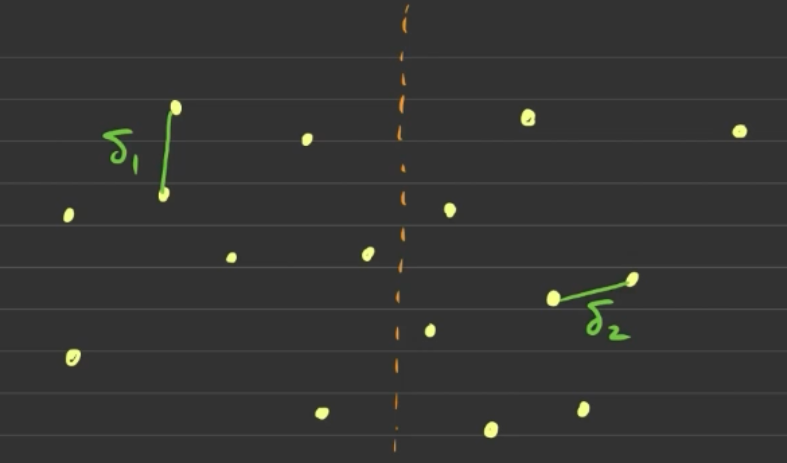
\includegraphics[scale=0.4]{img/closest_point.png}
      \caption{} 
      \label{fig:closest_point}
    \end{figure}

    We just have to check those with distance at most $\delta = \min\{\delta_1, \delta_2\}$ from each point. Furthermore, we can discard all points that are too far away from the boundary. However, all $N$ points could like in the relevant space, leading to $O(N^2)$ computations of distance. 

    \begin{figure}[H]
      \centering 
      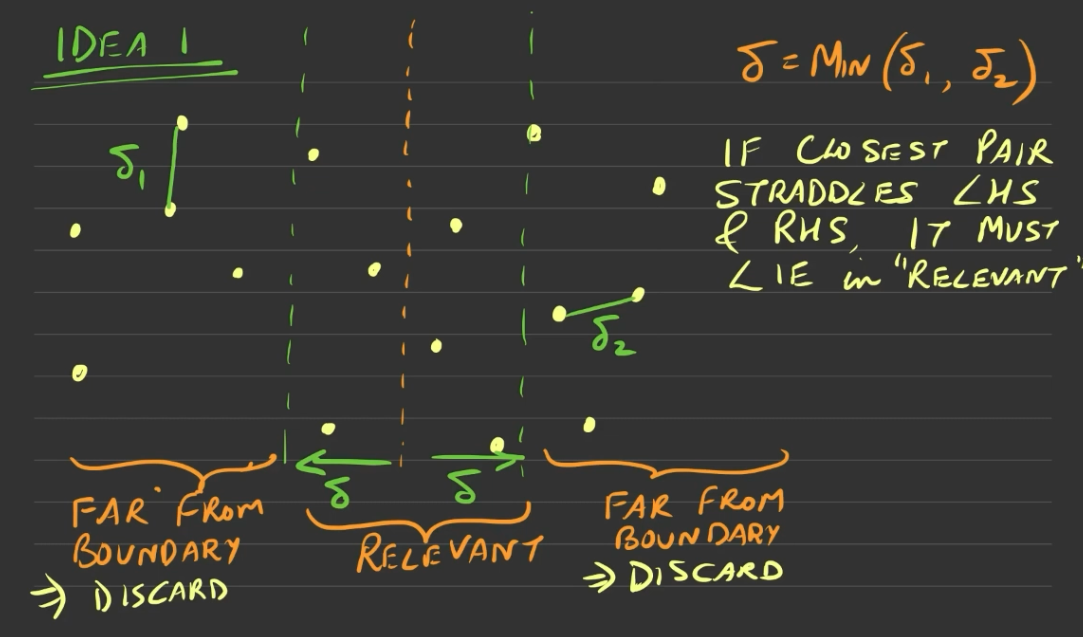
\includegraphics[scale=0.4]{img/cp2.png}
      \caption{} 
      \label{fig:closest_point2}
    \end{figure}

    Therefore, we want to incorporate vertical distances and tile our relevant space into square of side length $\delta/2$.  

    \begin{figure}[H]
      \centering 
      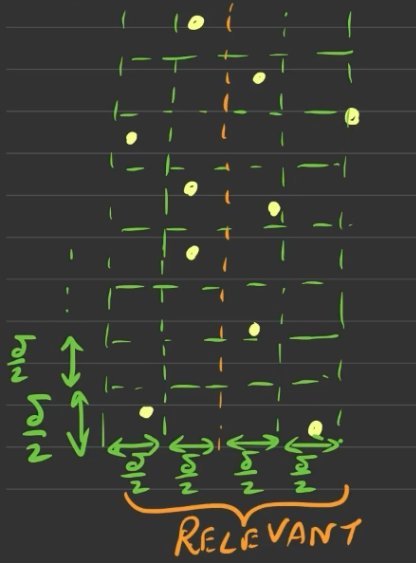
\includegraphics[scale=0.4]{img/cp3.png}
      \caption{} 
      \label{fig:closest_point3}
    \end{figure}

    We claim that each square has at most 1 point, since if there were two, then their distance would be less than $\delta / \sqrt{2}$, which contradicts the distance between the two points being greater than $\delta$. Therefore given a point, we only need to check a bounded constant. 

    \begin{figure}[H]
      \centering 
      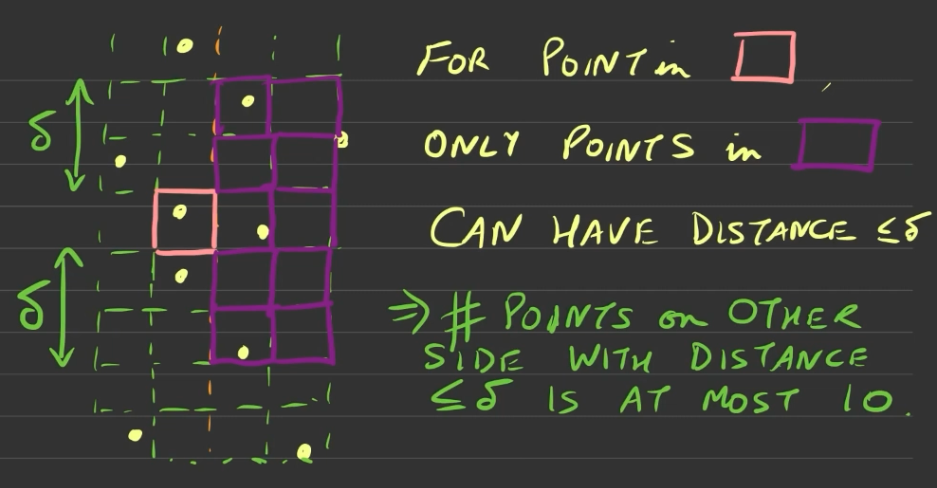
\includegraphics[scale=0.4]{img/cp4.png}
      \caption{The number of points on the other side with distance $\leq \delta$ is at most $10$. If we are more careful, we can reduce the number down to $7$. } 
      \label{fig:closest_point4}
    \end{figure}

    It turns out that we just need to compute $5N = (N/2) \cdot 10$ distances at most, and now our question reduces to how do we find these 5 points? Well we can first sort the points on the left and right by their y-coordinates, so we can just take a sliding window that encapsulates these points on the right for every on the left. The pointers of the sliding window should point to a point where the y-coordinate is at most $\delta$ away, and this can be done in constant time. Therefore, our recurrence relation is  

    \begin{equation}
      T(N) = 2 T(N/2) + O(N \log{N}) \implies T(N) = O(N \log^2 {N})
    \end{equation}
    
    This sorting along the y-coordinates is a bottleneck, but we can just shove this into the recursion step by telling the left and right to not just return the $\delta_1, \delta_2$, but also the points sorted in the y-coordinate. Then at the end of the merge, we also merge the lists $L, R$ so that $S = L \cup R$ is sorted on $y$, which also takes $O(N)$ and doesn't add extra runtime on the merge step. This reduces the runtime to $O(N \log{N})$. 

    \begin{algo}[Closest Pair of Points]
      The next problem simply takes a series of points and calculates the closest pair of points. This can be done trivially in $O(N^2)$ by taking all combinations, but with clever divide and conquer, we can reduce this down. 
      \begin{algorithm}[H]
        \caption{Closest Pair of Points}
        \label{alg:closest_pair}
        \begin{algorithmic}
          \Require{$N$ points $\{(x_i, y_i)\}$.}
          \State 
          \Function{ClosestPair}{P} 
            \State Sort points by x-coordinate. \Comment{Bottleneck of $O(N \log{N})$}
            \If{len(P) = 2} 
              \State \Return $d(p_1, p_2)$, sorted $P$ by y-coord
            \EndIf

            \State $\delta_1, L \gets$ ClosestPair($P_L$)
            \State $\delta_2, R \gets$ ClosestPair($P_R$)
            \State $\delta = \min\{\delta_1, \delta_2\}$ 
            \State min $\gets \delta$
            \For{$l \in L$ s.t. distance to boundary $\leq \delta$} \Comment{$O(N)$ iterations}
              \State $W_l \gets \delta$-window of points in $R$ around $l$. \Comment{Can be done in $O(1)$ using sliding window.}
              \For{$r \in W_l$} \Comment{This is bounded by $O(10)$}
                \If{$d(p, l) < \delta$} 
                  \State min $\gets d(p, l)$
                \EndIf
              \EndFor
            \EndFor

            \State merge $L$ and $R$ into sorted $S$ \Comment{O(N)} 

            \State \Return{min, S}
          \EndFunction
        \end{algorithmic}
      \end{algorithm}
    \end{algo}

  \subsection{Multiplication}

    \subsubsection{Karatsuba Algorithm}


    \subsubsection{Strassen Algorithm}

      We can solve matrix multiplication of two $N \times N$ matrices in a slightly more clever way than $O(N^3)$. Note that we can take the $2 \times 2$ block form of matrices $A, B$ and multiply them to get $C = AB$, where 
      \begin{align}
        C_{11} & = A_{11} B_{11} \cdot A_{12} B_{21} \\ 
        C_{12} & = A_{11} B_{12} \cdot A_{12} B_{22} \\ 
        C_{21} & = A_{21} B_{11} \cdot A_{22} B_{21} \\ 
        C_{22} & = A_{21} B_{12} \cdot A_{22} B_{22} 
      \end{align}

      This requires us to compute a total of $8$ $N/2 \times N/2$ multiplications and 4 additions, each of which is $O(N^2)$. Therefore, our recurrence relation is 
      \begin{equation}
        T(N) = 8 T(N/2) + O(N^2)
      \end{equation}

      Using the master theorem, we find that $a = 8 > 2^2 = b^c$, so our runtime is $O(N^{\log_{b} a}) = O(N^3)$, which brings us right back to where we started. The problem with this is that $a = 8$, which is large. If we could get $a = 7$, then this would be an improvement. We want to reduce this number of multiplications, and we can do this using the Strassen algorithm, which uses the following values.  
      \begin{align*}
        P_1 &= (a_{11} + a_{22}) (b_{11} + b_{22}) \\
        P_2 &= (a_{21} + a_{22}) b_{11} \\
        P_3 &= a_{11} (b_{12} - b_{22}) \\
        P_4 &= a_{22} (b_{21} - b_{11} \\
        P_5 &= (a_{11} + a_{12}) b_{22} \\
        P_6 &= (a_{21} - a_{11}) (b_{11} + b_{12}) \\
        P_7 &= (a_{12} - a_{22}) (b_{21} + b_{22}) 
      \end{align*}
      Then, we claim that we the entries of $C$ are 
      \begin{align*}
          c_{11} &= P_1 + P_4 - P_5 + P_7 \\
          c_{12} &= P_3 + P_5 \\
          c_{21} &= P_2 + P_4 \\
          c_{22} &= P_1 + P_3 - P_2 + P_6
      \end{align*}
      So we have reduced 8, 4 mult/add to 7, 18 mult/add. Addition is cheap and the number of additions is bounded, so now we have decreased $a$ to $7$.\footnote{We can reduce it even further, down to $2.37$. Whether $O(N^2)$ is possible is an open problem. } We can then solve the new recurrence relation 
      \begin{equation}
        T(N) = 7 T(N/2) + O(N^2) \implies O(N^{\log_2 7}) \approx O(N^{2.81})
      \end{equation}

  \subsection{Polynomial Multiplication with Fast Fourier Transform}

    Given as inputs $2$ degree $N$ polynomials, 
    \begin{align}
      A(x) & = a_0 + a_1x + a_2x^2 + \ldots + a_{n-1}x^{n-1} \\
      B(x) & = b_0 + b_1x + b_2x^2 + \ldots + b_{n-1}x^{n-1} 
    \end{align}
    we want to multiply them to $C(x) = A (x) B(x)$ defined 
    \begin{equation}
      C(x) = c_0 + c_1x + \cdots + c_{2n-2}x^{2n-2} 
    \end{equation}
    Clearly, we must multiply every coefficient in $A$ with $B$, which takes $O(N^2)$ time. It is also called the convolution operation. 
    \begin{align*}
      &\text{Convolution of } (a_0, a_1, \ldots, a_{n-1}) \text{ and } (b_0, b_1, \ldots, b_{n-1}) \\[1em]
      &c_0 = a_0 b_0 \\
      &c_1 = a_0 b_1 + a_1 b_0 \\
      &c_2 = a_0 b_2 + a_1 b_1 + a_2 b_0 \\
      &c_3 = a_0 b_3 + a_1 b_2 + a_2 b_1 + a_3 b_0 \\
      &\vdots \\
      &c_{2n-2} = a_{n-1} b_{n-1}
    \end{align*}

    We can actually compute this convolution of two vectors in $O(N \log{N})$ time using the FFT algorithm. Let's ease into this idea. 

    \begin{lemma}[Evauating a Polynomial at x]
      If we are given an $x$ and want to evaluate $A(x)$, we can just incrementally evaluate the terms up each degree in $O(N)$ time. 

      \begin{algorithm}[H]
        \caption{Evaluate polynomial $A(x)$ at $x=p$}
        \begin{algorithmic}[1]
        \State $S \gets a_0$
        \State $R \gets x$
        \For{$i = 1, 2, \ldots, n-1$}
            \State $S \gets S + a_i \cdot R$
            \State $R \gets R \cdot x$
        \EndFor
        \end{algorithmic}
      \end{algorithm}
    \end{lemma}

    Great, we can make some progress, but what does this have to do with finding the actual polynomial? Recall that from the fundamental theorem of algebra, a set of $n+1$ points will uniquely determine a $n$th degree polynomial. This at first glance doesn't help, since evaluating all $n+1$ points is $O(n^2)$, and even if we did, this doesn't really tell us how to reconstruct the polynomial in some fast time (e.g. matrix inversion won't work). But note that if we have a 1st degree polynomial, then evaluating it at $\pm1$ will retrieve the whole polynomial back
    \begin{equation}
      f(x) = a_0 + a_1 x \implies \begin{cases} f(+1) & = a_0 + a_1 \\ f(-1) & = a_0 - a_1 \end{cases} \implies \begin{cases} a_0 & = \frac{1}{2} \big( f(+1) + f(-1) \big) \\ a_1 = \frac{1}{2} \big( f(+1) - f(-1) \big) \end{cases}
    \end{equation}

    We can think of this as sort of our base case. For $N$th degree polynomials, we can divide it into a even and odd powers part. 
    \begin{align}
      A(x) & = a_0 + a_1 x + a_2 x^2 + \ldots \\ 
           & = (a_0 + a_2 x^2 + a_4 x^4) + x (a_1 + a_3 x^2 + a_5 x^4 + \ldots ) \\
           & = A_{\mathrm{even}} (x^2) + x A_{\mathrm{odd}} (x^2) 
    \end{align}
    where each of the splits have degree $N/2$. Then we want to evaluate the even and odd parts. 

    Let's jump ahead and focus on the problem of evaluating $A(x)$ of degree $N$ at the $N$th roots of unity. 

    \begin{example}
      For $N = 4$, we evaluate at $\pm 1, \pm i$. 
      \begin{equation}
        A(x) = (a_0 + a_2 x^2) + x (a_1 + a_3 x^2) 
      \end{equation}
      which gives us 
      \begin{align}
        A(+1) & = A_e (+1) + A_o (+1) \\ 
        A(-1) & = A_e (+1) - A_o (1) \\ 
        A(+i) & = A_e (-1) + i A_o (-1) \\ 
        A(-i) & = A_e (-1) - i A_o (-1) 
      \end{align}
      Note that even though we had $\pm i$ evaluated on $A$, they were all squared in each split so evaluating the 4th of unity, which we denote $U(4)$, has been reduced to finding $U(2)$ for each of the left and right polynomials. 
    \end{example}

    Therefore, to evaluate $A$ of degree $N$ at $U(N)$, it suffices to evaluate $A_e, A_o$ each at $U(N/2)$, followed by combing them using addition and multiplication, which turns out to be $O(N)$. 

    \begin{figure}[H]
      \centering 
      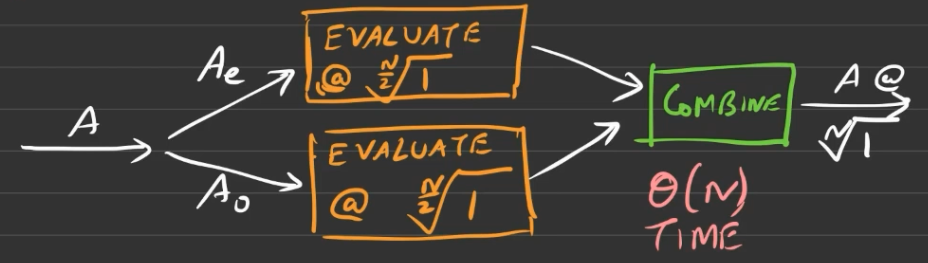
\includegraphics[scale=0.4]{img/fft.png}
      \caption{} 
      \label{fig:fft}
    \end{figure}

    \begin{algo}[Evaluate Nth Degree Polynomial at Nth Roots of Unity]
      
      \begin{algorithm}[H]
        \label{alg:unity}
        \begin{algorithmic}
          \Require{}
          \State 
          \Function{Func}{x}
          \EndFunction
        \end{algorithmic}
      \end{algorithm}
    \end{algo}

    Therefore, we have divided the problem of evaluating over $U(N)$ to be 
    \begin{equation}
      T(N) = 2 T(N/2) + O(N) \implies T(N) = O( N \log{N}) 
    \end{equation}

    So we have shown that in general, evaluating $N$ points of a polynomial takes $O(N^2)$ time, but if you're clever about what points to evaluate, you can get $O(N \log N)$. 

    Now going back to the original problem, we can evaluate $A(u), B(u)$ for $u \in U(N)$, and then multiply them to get $C(u)$. Great. Now to reconstruct the polynomial using the roots of unity, it turns out that there is a method in $O(N \log{N})$ time as well. 

\section{Greedy Algorithms}

  Greedy algorithms are easy to implement and easy to conceptualize, but they are often not correct. So the only interest in them is proving if they are correct. We have done greedy algorithms like Dijkstra and finding MSTs. Every step, greedy algorithms make an irrevocable decision of what to do and cannot undo it. That is, we cannot backtrack. In fact, some algorithms like Kruskal's algorithm for MSTs is precisely a greedy algorithm. 
  
  \begin{example}[Interval Scheduling]
    Let there be 1 classroom and $n$ courses, each with a start and end time $(s_i, e_i)$. We want to find the largest subset of courses that can be scheduled in a day such that they don't overlap. There are two things we want to do. How do we code this up? How do we show that a greedy algorithm will give a correct answer? Two greedy approaches are as follows. 
    \begin{enumerate}
      \item Sort them by the start times, and add them as long as they do not overlap with what you have. This will not work. 
      \item Sort them by the time interval lengths and keep adding them as long as they do not overlap with what you have. This will not work either. 
    \end{enumerate}
    It turns out that if we sort based on finish time, this will work. So why is this correct? Assume that the first $k$ decisions of this greedy algorithm are correct. Then, to find the next interval that we will include, the optimal algorithm must choose one that does not overlap with what we have. This is good since we do the same. The second part is that the next added interval must have the smallest end time $t$ from all viable left intervals. Assume that it was not and that the optimal next interval had end time $s > t$. Then, the next interval must start after $s$, but this also starts after $t$, so we are sacrificing unnecessary extra space. An optimal solution with the endpoint at $s$ can also be constructed with the same interval ending at $t$ without anything to lose. 

    \begin{algorithm}[H]
      \caption{Find Max Classes to Fit into 1 Room}
      \label{alg:class1}
      \begin{algorithmic}
        \Require{classes $C = \{(s_i, e_i)\}_i$ of type \texttt{List[tuple(int, int)]}}
        \Function{Schedule}{\texttt{C}}
          \State $\texttt{res} \gets \texttt{[]}$ 
          \State sort $C$ by increasing end time
          \For{$s, e \in C$} 
            \If{$s < \texttt{res[-1][-1]}$} \Comment{If start overlaps with previous end time}
              \State continue
            \EndIf
            \State add $(s, e)$ to res \Comment{Otherwise add class to final schedule}
          \EndFor
          \State \Return{\texttt{res}}
        \EndFunction
      \end{algorithmic}
    \end{algorithm}
    To get the run time, the sorting takes $O(n \log{n})$ time and iterating is $O(n)$, so a total of $O(n \log{n})$ time. 
  \end{example}

  \begin{example}[Classroom Scheduling]
    A slightly more practical example is that you have $n$ classes and you want to minimize the number of classrooms $m$. For this, you can really use any order. The general idea is 
    \begin{enumerate}
      \item Consider intervals in increasing start time $s_i$. 
      \item If it can be scheduled in an existing classroom, then schedule it there. 
      \item If not, then open a new classroom. 
    \end{enumerate}
    Even then, we can conduct a line search through all the time periods, incrementing the current number of classes if an incoming time is a start time and decrementing if it is an end time. We report the max $\Delta$ over all times. 

    This algorithm is correct since by definition, $\Delta$ is the lower bound for the number of classrooms needed and the greedy algorithm attains it. The greedy algorithm reports $\Delta$ since if it reported $\Delta +1$ classroom, then at some time $t$ it opened the $\Delta+1$th classroom. But this is impossible since this must mean that there are $\Delta + 1$ classrooms concurrently in use, contradicting our assumption that $\Delta$ is the optimal solution. 

    \begin{algorithm}[H]
      \caption{Minimizing Number of Rooms With $n$ Classes (Leetcode 253, Meeting Rooms II)}
      \label{alg:class_schedule}
      \begin{algorithmic}
        \Require{classes $C = \{(s_i, e_i)\}_i$ of type \texttt{List[tuple(int, int)]}}
        \Function{MeetingRooms}{$C$} 
          \State $\texttt{start} \gets$ all start times sorted increasing 
          \State $\texttt{end} \gets$ all end times sorted increasing 
          \State $\texttt{res} \gets 0$ \Comment{Our max classes count} 
          \State $\texttt{count} \gets 0$ \Comment{Our curr. classes count} 
          \State $\texttt{s}, \texttt{e} \gets 0$ \Comment{pointers for \texttt{start}, \texttt{end}} 

          \While{\texttt{s < len(start)}} \Comment{Don't need to check for \texttt{end} since}
            \If{\texttt{start[s] == \texttt{end[e]}}} \Comment{\texttt{start} will always finish faster.}
              \State \texttt{s += 1, e += 1} \Comment{One started and one ended, so don't change}
            \ElsIf{\texttt{start[s] > \texttt{end[e]}}} 
              \State \texttt{e += 1, count -= 1} \Comment{One ended, so decrement \texttt{count}}
            \ElsIf{\texttt{start[s] < \texttt{end[e]}}}
              \State \texttt{s += 1, count += 1} \Comment{One started, so increment \texttt{count}}
              \State \texttt{res = max(res, count)} \Comment{Update res if we got past it}
            \EndIf
          \EndWhile

          \State \Return{res}
        \EndFunction
      \end{algorithmic}
    \end{algorithm}

    The runtime is $O(n \log{n})$, which is to sort. However, you don't even need to sort since you can go through all intervals in any order and place it in an existing classroom or open a new classroom. 
  \end{example}

  The next one isn't as trivial, but requires us to devise a custom sorting method by comparing two sequences with a swap difference. 

  \begin{example}[Quiz Problem]
    Suppose you have $n$ questions with question $i$ having reward $r_i$, but the probability that you get it correct is $p_i$. You keep collecting the reward until you get one question wrong, and the game terminates. What order would you answer the questions in? 

    Suppose we have $q = (10, 5)$ and $r = (0.1, 0.2)$. 
    \begin{enumerate}
      \item If you choose the first and then second, then the expected return is 
        \begin{equation}
          10 \cdot 0.1 + 5 \cdot 0.1 \cdot 0.2 = 1.1 
        \end{equation}

      \item If you choose the second and then first, then the expected return is 
        \begin{equation}
          5 \cdot 0.2 + 10 \cdot 0.1 \cdot 0.2 = 1.2
        \end{equation}
    \end{enumerate}
    Clearly, finding all possibilities is too computationally expensive since it increases exponentially w.r.t. $n$. Intuitively, if I have a question with a high reward, I want to answer it first, but if I have a low probability of getting it correctly, then I can't answer future questions if I get it wrong. So I have to balance these two forces. So we want to sort the score of each question with some function $f(r_i, p_i)$, which is increasing in both $r_i$ and $p_i$. It is not $r_i p_i$, but this is a good start. 
    
    Rather, we can take a different approach. Assume that the tuples were sorted in some order, but this was not the optimal order. Then this indicates that we can swap to adjacent elements and it will get a better order. This is really like bubble sort, and now we need to find out the conditions on which it can be improved.  
    \begin{enumerate}
      \item If we answer $q_1 \rightarrow q_2 \rightarrow q_3 \ldots$, our expected reward is 
        \begin{equation}
          \mathbb{E}[R] = r_1 p_1 + r_2 p_1 p_2 + r_3 p_1 p_2 p_3 
        \end{equation}
      \item If we swap $q_2$ and $q_3$ and answer $q_1 \rightarrow q_3 \rightarrow q_2 \ldots$, then our expected reward is 
        \begin{equation}
          \mathbb{E}[R] = r_1 p_1 + r_3 p_1 p_3 + r_2 p_1 p_2 p_3 
        \end{equation}
      Note that the swap does not affect higher order terms. Doing some algebra, the swap is better iff 
      \begin{equation}
        r_2 p_2 (1 - p_3) < r_3 p_3 (1 - p_2) \implies \frac{r_2 p_2}{1 - p_2} < \frac{r_3 p_3}{1 - p_3}
      \end{equation}
      where the final swap saves computational time since we can compute for a single element rather than comparing pairwise elements. So, we sort it (in descending order!) according to these values to maximize this value. Note that the numerator measures your expected reward, while the denominator measures the probability of you screwing up. 

    \end{enumerate}
  \end{example}

  Not all greedy problems admit to scoring functions however. This was just one example. 

  \begin{example}[Minimizing Max Lateness]
    Suppose there are $n$ jobs that all come in at once at time $0$, with job $j$ having length $p_j$ and deadline $d_j$. We want to schedule the order of jobs on one machine that can handle one job at a time, where you must minimize the maximum lateness, where the lateness of job $i$ is $\max\{f_i - d_i, 0\} = [f_i - d_i]^+$. 

    For example, given jobs $(p, d) = \{(10, 9), (8, 11)\}$, we can run it in two ways. 
    \begin{enumerate}
      \item Running 1 then 2. The first job finishes at $10$ and the second at $18$. The lateness is $10 - 9 = 1$ and $18 - 11 = 7$ respectively, so the maximum lateness is $7$. 
      \item Running 2 then 1. The first job finishes at $8$ and the second at $18$. The lateness is $0$ and $18 - 9 = 9$, so the maximum lateness is $9$.  
    \end{enumerate}
    Therefore, $1 \rightarrow 2$ beats $2 \rightarrow 1$. Clearly, brute forcing this over $N!$ jobs orderings is unfeasible, but there is a greedy approach to this. We can 
    \begin{enumerate}
      \item schedule jobs in increasing order of deadlines. 
      \item try to exchange by taking a sequence, swapping it, and computing the score like we did for previous examples. 
    \end{enumerate}
    Both lead to the same score/principle that we should schedule jobs in increasing order of deadlines. Let's prove this by taking jobs $i$ and $j$, where $d_j \leq d_i$. Then, if we schedule $i \rightarrow j$, then we have 
    \begin{align}
      l_i & = [t + p_i - d_i]^+ \\
      l_j & = [t + p_i + p_j - d_j]^+ 
    \end{align}
    with $l_j$ being the greatest late time. If we did $j \rightarrow i$, then we have 
    \begin{align}
      \hat{l}_j & = [t + p_j - d_j]^+ \\
      \hat{l}_i & = [t + p_i + p_j - d_i]^+ 
    \end{align}
    with $\hat{l}_i$ being the greatest late time. But this is a good sacrifice since we can see that both 
    \begin{equation}
      l_j > \hat{l}_j \text{ and } l_j > \hat{l}_i
    \end{equation}
    meaning that if we swap, then we will decrease the lateness of $j$ at the smaller cost of increasing that of $i$. Therefore, $j \rightarrow i$ is better. Note that even though the end times of the second job will always be the same between the two choices, starting with $j$ will give a later deadline time. So this means that in the optimal solution, we have to place them in this order of deadlines since we can always improve them by swapping. 
  \end{example}

  \begin{example}[Gift Wrapping a Convex Hull]
    Given $n$ points in $\mathbb{R}^2$, we want to find the subset of points on the boundary of its convex hull. We can intuit this by taking the bottom most point and imagine ``wrapping'' a string around the entire region.\footnote{This is called the gift wrapping algorithm.} Here's a basic fact. If we have a point $p_1 = (x_1, y_1)$ and we're looking at $p_2 = (x_2, y_2)$, and then $p_3 = (x_3, y_3)$ shows up, then we can look at the cross product 
    \begin{equation}
      P = (x_2 - x_1) (y_3 - y_1) - (y_2 - y_1)(x_3 - x_1) 
    \end{equation}
    and if $P > 0$, then $p_3$ is counterclockwise from $p_2$. The algorithm is as such. 
    \begin{enumerate}
      \item You choose the bottommost point and label it $p_1$. 
      \item You construct a vector pointing to the right and start turning it counterclockwise until it hits the first point. This can be done by iterating through all of the $n$ points and computing the angle. 
        \begin{equation}
          \tan{ \theta} = \frac{y_i - y_1}{x_i - x_1}
        \end{equation}
      and the points with the smallest such tangent value will be the desired point, which will be $\Theta(n)$. We set this point to be $p_2$ and claim that $p_1, p_2$ is in the convex hull. This is true since all point must lie above the line $p_1 p_2$. Now you do the same thing with $p_2$ starting with a vector facing to the right and rotating it left until it hits the first peg. Once you get to the topmost point, you can start the vector from the right and rotate it counterclockwise, but this is an implementation detail. 

      If your convex hull has $L$ vertices, then this algorithm will have $O(n L)$, which will be $O(n^2)$ worst case but if we sample uniformly, then we have $L \approx \log{n}$ and on average it is $O(n \log{n})$. 
    \end{enumerate}
    A lot of geometric algorithms is output sensitive. 
  \end{example}

  \begin{example}[Convex Hull with Graham Scan]
    In fact, we can take a different approach and get $O(n \log{n})$ time. 
    \begin{enumerate}
      \item You still start with $p_1$ with the minimum y-coordinate and we sort in increasing $\theta_i = \arctan \frac{y_i - y_1}{x_i - x_1}$. 
      \item Then it will walk from $p_i$ to $p_{i+1}$ and check at $p_{i+1}$ if it is on the convex hull or not. 
        \begin{enumerate}
          \item If you turned counterclockwise to go to $p_{i+1}$ then it's good and you're on the convex hull. 
          \item If you turned clockwise it is bad, and $p_i$ is not on the convex hull, so remove $p_i$. However, $p_{i-1}$ could also be clockwise as well, so you must backtrack and keep on removing points until you find a point $p_j$ such that the previous turn is counterclockwise. 
        \end{enumerate}
        Note that this is implemented as a stack. 
    \end{enumerate}
    This can be calculated in $O(1)$ by the previous cross product formula. 
    \begin{figure}[H]
      \centering 
      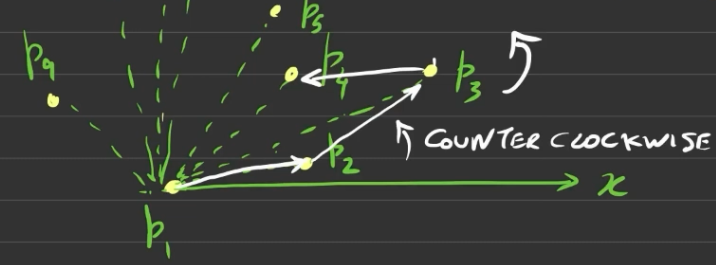
\includegraphics[scale=0.4]{img/graham.png}
      \caption{Overview of the steps mentioned above. } 
      \label{fig:graham}
    \end{figure}
    \begin{algorithm}[H]
      \caption{Finding Convex Hull with Graham Scan}
      \label{alg:graham}
      \begin{algorithmic}
        \Require{$p_1, \ldots, p_n \in \mathbb{R}^2$}
        \Function{Graham}{$\mathbf{p}$} 
          \State s $\gets$ stack()
          \State push $p_1, p_2$ onto s 
          \For{$i = 3, 4, \ldots, n$}
            \State push $p_i$ onto stack 
            \While{top 3 on stack are clockwise}
              \State pop second from top point 
            \EndWhile
          \EndFor 
          \State \Return{s} 
        \EndFunction
      \end{algorithmic}
    \end{algorithm}
    Note that once we have 3 points, the first three in the stack will always be counterclockwise, so we will never need to check if there are enough points in the stack. Even in the beginning, the next point (third) added is guaranteed to be counterclockwise because of ordering. Note that even though we might do a bunch of pushes and pops, the maximum number of pushes we can do is $n$ and pops is $n$, so this is $O(n)$. In fact, the bottleneck is the sorting, which is $O(n \log{n})$, so the total runtime is $O(n \log{n})$. 
  \end{example}

\section{Graphs}

    A huge portion of problems can be solved by representing as a \textit{graph} data structure. In here, we will explore various problems that can be solved through \textit{graph algorithms}. 

  \subsection{Representations and Properties}

    All graphs consist of a set of vertices/nodes $V$ and edges $E$. This tuple is what makes up a graph. We denote $|V| = n, |E| = m$. 

    \begin{definition}[Undirected Graphs]
      An \textbf{undirected graph} $G(V, E)$ is a tuple, where $V = \{v_1, \ldots, v_n\}$ is the vertex set and $E = \{\{v_i, v_j\}\}$ is the edge set (note that it is a set of sets!). 
      \begin{enumerate}
        \item The \textbf{degree} $d_v$ of a vertex $v$ is the number of edges incident to it. 
        \item A \textbf{path} is a sequence of vertices where adjacent vertices are connected by a path in $E$. It's \textbf{length} is the number of edges in the path. 
        \item A \textbf{cycle/circuit} is a path that has the same start and end. 
        \item A graph is \textbf{connected} if for every pair of vertices $e_i, e_j \in E$, there is a path from $e_i$ to $e_j$. 
        \item A \textbf{connected component} is a maximal subset of connected vertices. 
      \end{enumerate}
    \end{definition}

    \begin{definition}[Directed Graph]
      A \textbf{directed graph} $G(V, E)$ is a tuple, where $V = \{v_1, \ldots, v_n\}$ is the vertex set and $E = \{(v_i, v_j)\}$ is the edge set (note that it is a set of tuples, so $(i, j) \neq ( j, i)$).
      \begin{enumerate}
        \item The \textbf{in/out degree} $d_{v, i}, d_{v, o}$ of a vertex $v$ is the number of edges going in to or out from $v$. 
        \item A \textbf{path} is a sequence of vertices where adjacent vertices are connected by a path in $E$. It's \textbf{length} is the number of edges in the path. 
        \item A \textbf{cycle/circuit} is a path that has the same start and end. 
        \item A directed graph is \textbf{strongly connected} if for every pair of vertices $e_i, e_j \in E$, there is a path from $e_i$ to $e_j$.\footnote{Obviously, a connected undirected graph is also strongly connected.}
        \item A \textbf{strongly connected component} is a maximal subset of connected vertices. 
      \end{enumerate}
    \end{definition}

    In fact, from these definitions alone, we can solve an ancient puzzle called \textit{the Bridges of Konigsberg}. Euler, in trying to solve this problem, had invented graph theory. 

    \begin{example}[Bridges of Konigsberg]
      Is there a way to walk that crosses each bridge \textit{exactly} once? 
      \begin{figure}[H]
        \centering 
        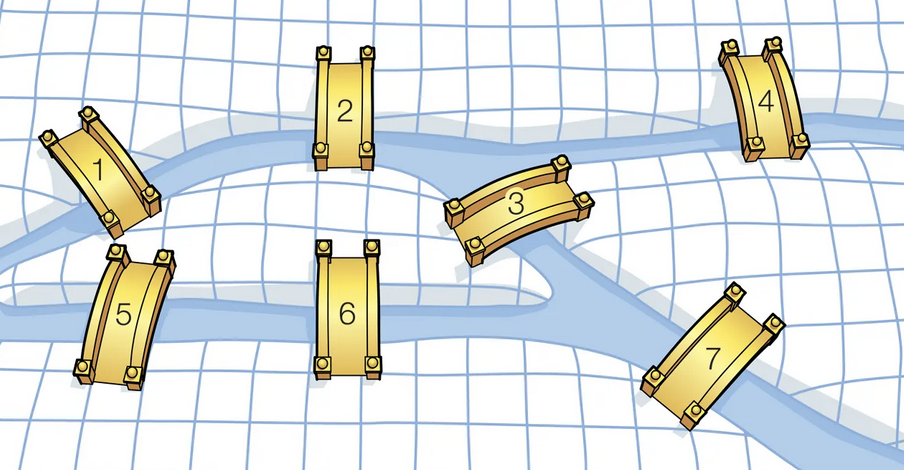
\includegraphics[scale=0.4]{img/bridges.png}
        \caption{Bridges of Konigsberg} 
        \label{fig:bridges}
      \end{figure}
      It can be decomposed into this undirected graph. 
      \begin{figure}[H]
        \centering 
        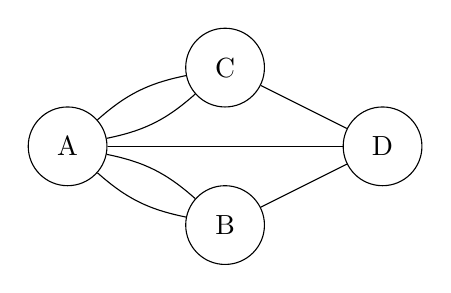
\begin{tikzpicture} 
          \tikzstyle{every node}=[circle, draw, minimum size=1cm]
          
          \node (A) at (0,0) {A};
          \node (B) at (2,-1) {B};
          \node (C) at (2,1) {C};
          \node (D) at (4,0) {D}; 
                
          \draw (A) to[bend left=15] (B);
          \draw (A) to[bend right=15] (B);
          \draw (A) to[bend left=15] (C);
          \draw (A) to[bend right=15] (C);
          \draw (A) -- (D);
          \draw (B) -- (D);
          \draw (C) -- (D);
        \end{tikzpicture}
        \caption{Graph representation. } 
        \label{fig:bridge_graph}
      \end{figure}
      Euler's observation is that except for start and end points, a talk leaves any vertex by different edge that the incoming edge. Therefore, the degree (number of edges incident on it) must have an even number, so all but 2 vertices must have an even degree. Since every vertex has an odd degree, there is no way of doing it. 
    \end{example}

    In addition to the \textit{adjacency list} representation, another way in which we represent a directed graph is through \textit{adjacency matrices}. 

    \begin{definition}[Adjacency Matrix]
      In a finite directed graph $(V, E)$, we can construct a bijection from $V$ to the natural numbers and so we label each element in $V$ with $i \in \mathbb{N}$. Then, we can construct a matrix $A$ such that 
      \begin{equation}
        A_{ij} = \begin{cases} 1 & \text{ if } (i, j) \in E \\ 0 & \text{ if } (i, j) \not\in E \end{cases}
      \end{equation}
    \end{definition}

    While the adjacency matrix does have its advantages and has a cleaner form, usually in sparse graphs this is memory inefficient due to there being an overwhelming number of $0$s. 

    \begin{definition}[Trees]
      An undirected graph $G(V, E)$ is a \textbf{tree} if 
      \begin{enumerate}
        \item $G$ is connected. 
        \item $G$ has no cycles.\footnote{This makes sense, since to get back to a previous vertex you must backtrack.}
      \end{enumerate}
      Removing the first requirement gives us the definition of a \textbf{forest}, which is a collection of trees. Conversely, if $G(V, E)$ is connected  and $|E| = n - 1$, then $G$ is a tree. 
    \end{definition}

    \begin{theorem}[Properties of Trees]
      If $G(V, E)$ is a tree, then 
      \begin{enumerate}
        \item There exists a $v \in V$ s.t. $d_v = 1$, called a \textbf{leaf node}. 
        \item $|E| = |V| - 1 = n - 1$. 
      \end{enumerate}
    \end{theorem}
    \begin{proof}
      The outlines are quite intuitive. 
      \begin{enumerate}
        \item There must be some leaf node since if there wasn't, then we would have a cycle. We can use proof by contradiction. 
        \item We can use proof by induction. We start off with one vertex and to construct a tree, we must add one edge and one vertex at every step, keeping this invariant.  
      \end{enumerate}
    \end{proof}

  \subsection{Exploration}

    Given two $v, s \in V$ either directed or undirected, how can we find the shortest path from $v$ to $s$? We can do with either with DFS or BFS. 

    \begin{definition}[DFS]
      The recursive algorithm is 
      \begin{lstlisting}
        visited = set() 
        def dfs(start): 
          if start not in visited: 
            visited.add(start) 
            # do something 
            neighbors = ... 
            for neighbor in neighbors: 
              dfs(neighbor)
      \end{lstlisting}

      The iterative algorithm uses a stack, which mirrors the function call stack. 
      \begin{lstlisting}
        visited = set() 

        def dfs(start): 
          toExplore = [] 
          current = start; 
          toExplore.append(current) 
          visited.add(current) 
          while toExplore: 
            current = toExplore.pop() 
            # Do something
            neighbors = ... 
            for neighbor in neighbors: 
              if neighbor not in visited: 
                visited.add(neighbor) 
                toExplore.append(neighbor)
      \end{lstlisting}
    \end{definition}

    \begin{theorem}[Runtime of DFS]
      The runtime of DFS is $O(n+m)$. 
    \end{theorem}
    \begin{proof}
      
    \end{proof}

    \begin{definition}[BFS]
      The iterative version is shown.\footnote{The recursive version of BFS is very nontrivial.}
      \begin{lstlisting}
        visited = set() 
        def bfs(start): 
          toExplore = collections.deque() 
          current = start; 
          toExplore.append(current) 
          visited.add(current) 
          while toExplore: 
            current = toExplore.popleft() 
            # Do something 
            neighbors = ... 
            for neighbor in neighbors: 
              if neighbor not in visited: 
                visited.add(neighbor) 
                toExplore.append(neighbor)
      \end{lstlisting}
    \end{definition}

    \begin{theorem}[Runtime of BFS]
      The runtime of BFS is $O(n+m)$. 
    \end{theorem}
    \begin{proof}
      To get the running time, we know that each vertex is popped only once from the queue, giving us $O(n)$. For each pop, we are exploring all the neighbors of $V$. 
      \begin{align}
        O \bigg( \sum_{v \in V} | \text{neighbors of } v| + 1\bigg) & = O \bigg( \sum_{v \in V} d_v + 1 \bigg) \\
                                             & = O (2 |E| + |V|) = O(m + n )
      \end{align}
      which is linear in input size!  
    \end{proof}

    The more straightforward application is in reachability. 

    \begin{example}[Reachability]
      Given a directed graph and a node $v$, find all nodes that are reachable from $v$. 
    \end{example}

    \begin{exercise}
      Prove that in any connected undirected graph $G = (V, E)$ there is a vertex $v \in V$ s.t. $G$ remains connected after removing $v$. 
    \end{exercise}
    \begin{proof}
      Let $u$ be such a leaf node of $T$, and let $G'$ be the subgraph of $G$ resulting by removing $u$ and its incident edges from $G$.
      For sake of contradiction,\footnote{We provide an alternative direct proof as follows: Since $G$ is given to be connected, $T$ contains all vertices of $G$. Let $T'$ be the BFS tree minus $u$ and its single incident edge connecting it to its parent in $T$. Since $u$ is a leaf, $T'$ remains a connected tree with all other vertices of $G$. The edges of $T'$ exist in $G'$, so $G'$ is connected.} suppose $G'$ has more than one connected component.
      Let $C$ be a connected component in $G'$ that does not contain $s$, the root of the BFS tree $T$.
      Since $G$ was connected before the removal of $u$, it must be that every path from $s$ to any vertex $v$ in $C$ includes $u$ (otherwise there would remain a path from $s$ to $v$ in $G'$ and $s$ would be in $C$).
      Then $u$ is the only vertex not in $S$ with edges to vertices in $S$, so all vertices in $C$ must be ``visited'' during BFS only after visiting $u$. Furthermore, the vertices of $S$ must be in the subtree of $T$ rooted at $u$. But $u$ is a leaf, which is a contradiction.
    \end{proof}

    \begin{exercise}
      Two parts. 
      \begin{enumerate}
        \item Give an example of a strongly connected directed graph $G = (V, E)$ s.t. that every $v \in V$, removing $v$ from $G$ gives a directed graph that is not strongly connected. 
        \item In an undirected graph with exactly two connected components, it is always possible to make the graph connected by adding only one edge. Give an example of a directed graph with two strongly connected components such that no addition of one edge can make the graph strongly connected.
      \end{enumerate}
    \end{exercise}
    \begin{proof}
      Listed. 
      \begin{enumerate}
        \item A graph whose edges form a cycle, having at least three nodes.
        \item Two strongly connected components with no edges between them.
      \end{enumerate}
    \end{proof}
    
  \subsection{Directed Acyclic Graphs and Topological Sorting}

    \begin{definition}[Directed Acyclic Graph]
      A DAG is a directed graph that has no cycles. Note that a DAG must have a node that has no in-edges. 
    \end{definition}

    To determine if a graph is a DAG, then we can brute force it by taking a node $s \in V$, running DFS/BFS, and if a neighbor is already in visited, return False. Then go through this for all starting nodes $s \in V$. This again has quadratic runtime. Can we do better? This introduces us to topological sorting. 

    It may be helpful to take a graph $G(V, E)$ and induce some partial order on the set of nodes $V$ based off of $E$. It turns out that we can do this for a specific type of graph. 
    
    \begin{definition}[Topological Sort]
      Given a directed acyclic graph (DAG), a linear ordering of vertices such that for every directed edge $u-v$, vertex $u$ comes before $v$ in the ordering is called a \textbf{topological sort}. It satisfies the facts: 
      \begin{enumerate}
        \item The first vertex must have an in-degree of $0$. 
        \item A topological sort is not unique. 
      \end{enumerate}
    \end{definition}

    \begin{example}[Simple Topological Sort]
      The graph below 
      \begin{figure}[H]
        \centering 
        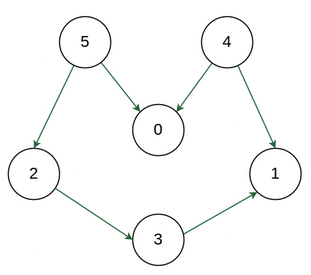
\includegraphics[scale=0.55]{img/top_sort.png}
        \caption{} 
        \label{fig:top_sort}
      \end{figure}
      can have the two (not exhaustive) topological sortings. 
      \begin{enumerate}
        \item $[5, 4, 2, 3, 1, 0]$
        \item $[4, 5, 2, 3, 1, 0]$
      \end{enumerate}
    \end{example}

    To determine if a graph is a DAG, note the following theorem. 

    \begin{theorem}[Topological Order and DAGs]
      $G$ has a topological order if and only if it is a DAG. 
    \end{theorem}
    \begin{proof}
      To prove that a DAG has a topological order, we use induction. Pick a $v$ such that its indegree is $0$. Then, delete $v$, and therefore $G \setminus v$ is also a DAG with a topological order since we are only deleting edges. We keep going. 
    \end{proof}

    Therefore, if we can successfully topologically sort, we know it is a DAG. So we can kill two birds with one stone. Let's see how this is implemented. We can do it iteratively and recursively (the proof above should hint that this can be recursive). 

    \begin{algo}[Iterative Topological Sort, Determine If Graph is DAG]
      The general idea is that we first find the node that as $0$ in-degree. From here, we can do DFS, and when we run out of neighbors to explore, then we push this into a queue. This is essentially a post-order traversal, where at the end are going to be the end nodes with no more neighbors, and the node we started from will be added last. Then we loop through and do this for all start nodes. We first need a slightly modified form of DFS. 

      \begin{algorithm}[H]
        \label{alg:iterative_top_sort}
        \begin{algorithmic}[1]
          \Require{Nodes $V$, adjacency list $E$}
          \State visited $\gets$ set()
          \State res $\gets$ stack() 
          \State is\_acyclic $\gets$ True

          \Function{DFS}{$v \in V$}
            \If{$v \neq $ visited}
              \State add $v$ to visited 
              \State $N_v \gets$ neighbors of $v$ 
              \For{$n \in N_v$}
                \If{$n \in $ visited} 
                  \State is\_acyclic $\gets$ False 
                \EndIf
                \State \Call{DFS}{$n$}
              \EndFor 
              \State push $v$ onto res
            \EndIf
          \EndFunction

          \State 

          \Function{TopologicalSort}{V, E}
            \For{$v \in V$} 
              \State DFS($v$)
            \EndFor
            \If{! is\_acyclic}
              \State \Return{False}
            \EndIf
            \State \Return{reversed of res}
          \EndFunction
        \end{algorithmic}
      \end{algorithm}
      Note that this runtime is $O(|V| + |E|)$ since we are just running DFS with a constant amount of work on top of each call. 
    \end{algo}

    \begin{algo}[Recursive Topological Sort]
      We want to see that while $G$ is nonempty, we want to find the $v \in V$ such that it has indegree $0$. Then place $v$ next in order, and then delete $v$ and all edges out of $v$. The problem is finding which vertex has indegree $0$ (if we brute force it by looking through all remaining nodes and edges, you have quadratic runtime). To do this fast, the idea is 
      \begin{enumerate}
        \item initially scan over all edges to store the indegrees of every node to a list \texttt{indeg}. 
        \item store all nodes with indegree $0$ to a queue. 
        \item Run through the queue, and during each loop, when we remove a node, we look at all of its out-nodes $s$ and decrement \texttt{indeg[s]}. If \texttt{indeg[s] = 0}, then add it to the queue. 
      \end{enumerate}
      \begin{algorithm}[H]
        \label{alg:recursive_top_sort}
        \begin{algorithmic}[1]
          \Require{Nodes $V$, Edges $E$}
          \State $q \gets$ queue() 
          \State indeg $\gets$ list() 
          \State visited $\gets$ 0
          \Function{Recur}{x}
            \State initialize the indeg and $q$ 

            \While{q is nonempty} 
              \State $v \gets$ pop(q) 
              \State visited += 1 
              \For{each $w \in E[v]$} 
                \State indeg[w] -= 1 
                \If{indeg[w] = 0} 
                  \State push w into q 
                \EndIf
              \EndFor
            \EndWhile

            \If{visited != |V|} 
              \State \Return{False}
            \EndIf

            \State \Return{True}
          \EndFunction
        \end{algorithmic}
      \end{algorithm}
      Notice that the inner for loop is $O(d(v) + 1)$, while we run over all $n$. So really, we are doing $O(n(d(v) + 1)) = O(m + n)$, where the plus $n$ comes from the constant work we are doing for each node. Note that if we have a non-DAG, then at some point the queue will be empty but we haven't processed all the vertices, at which point we can declare failure. 
    \end{algo}

    To end this, we can make a general statement about all directed graphs. 

    \begin{theorem}
      Every directed graph is a DAG of strongly connected components (SCC). 
    \end{theorem}

    This gives us a way to represent a directed graph with a collection of DAGs.\footnote{In fact, this Kosaraju's algorithm, can be done in linear time, though it is highly nontrivial.} An extension of topological sort is making a \textit{BFS tree}, which partitions a graph into layers that represent the number of steps required to go from a source vertex to a node. 

    \begin{algo}[BFS Tree]
      To construct a BFS tree, we just need to slightly modify the original BFS code.
      \begin{algorithm}[H]
        \label{alg:bfs_tree}
        \begin{algorithmic}[1]
          \Require{Nodes $V$, adjacency list $E$}
          \State visited = set() 
          \State layers = $\{v : 0 \mid v \in V \}$
          \Function{BFS}{start}
            \State layer $\gets 0$ 
            \State toExplore $\gets$ queue() 
            \State add (start, layer) to toExplore 
            \State add start to visited
            \While{toExplore} 
              \State curr, layer = pop from toExplore 
              \State layers[curr] = layer 
              \For{$n \in$ neighbors of curr} 
                \If{$n \not\in$ visited} 
                  \State add $n$ to visited 
                  \State add $(n, layer+1)$ to visited 
                \EndIf
              \EndFor
            \EndWhile 
          \EndFunction
        \end{algorithmic}
      \end{algorithm}
      This is simply BFS with constant extra work so it is $O(n + m)$. 
    \end{algo}

    So, a BFS tree is really just another way to topologically sort. Note the following properties. 
    \begin{enumerate}
      \item In a directed graph, no nodes can jump from layer $i$ to layers $j > i+1$, since if it could, then it would be in layer $i+1$. However, nodes can jump from layer $j$ back to any layer $i < j$, even skipping layers. 
      \item In a directed graph, going forward is the same as going back, so nodes can jump at most one layer forwards or backwards. 
    \end{enumerate}


    \begin{exercise}[DPV 3.16]
      Suppose a CS curriculum consists of $n$ courses, all of them mandatory. The prerequisite graph $G = (V,E)$ has a node for each course, and an edge from course $v$ to course $w$ if and only if $v$ is a prerequisite for $w$. Note this is a directed acyclic graph (DAG). In order for a student to take a course $w$ with prerequisite $v$, they must take $v$ in an earlier semester. Find an algorithm that works directly with this graph representation, and computes the minimum number of semesters necessary to complete the curriculum, under the assumption any number of courses can be taken in one semester. The running time of your algorithm should be $O(n+m)$, where $n$ and $m$ are the numbers of vertices and edges in $G$, respectively.
    \end{exercise}
    \begin{proof}
      For each vertex, we want to find the longest path leading to it: if there is a path leading to a node, then all of the courses in the path should be taken sequentially. Perform a topological sort of $G$'s nodes and label them $1$ through $n$. Then, we go through the nodes in the resulting topological order. For each vertex, we assign the minimum number of semesters required to take it: if there are no prerequisites, we assign 1, and if there are prerequisites, we assign 1 plus the maximum value assigned to its prerequisite nodes.
      
      \textit{Implementation details}: If the input is in adjacency list format, then we do not have access to the \emph{incoming} edges to a node (its prerequisites). By exploring the entire graph with BFS calls, we can compute the list of incoming edges to every vertex in $O(n+m)$ time. These details are not required. If the input is in adjacency matrix format, for each node it takes $O(n)$ time to find its incoming edges, so the total running time is $O(n^2)$.
    \end{proof}

    \begin{exercise}[DPV 3.22] 
      Give an efficient algorithm that takes as input a directed graph $G = (V,E)$, and determines whether or not there is a vertex $s \in V$ from which all other vertices are reachable.
    \end{exercise}
    \begin{proof}
      We first build the DAG representation of the SCCs of $G$ in $O(m+n)$ time, as described in lecture. This graph is a DAG where each SCC of $G$ is represented by a single node. We return true if this DAG has exactly one node with no incoming edges (i.e., exactly one source node), and return false otherwise.

      \textit{Correctness.} Let $u$ be a vertex in an SCC that is a source node in the DAG representation. If there is a path in $G$ from a vertex $v$ not in the SCC of $u$ to $u$, then there must be an edge (corresponding to an edge in this path) into the SCC of $u$ in the DAG, which contradicts that the node has no incoming edges. Thus, if there are two source SCCs in the DAG, no vertex of $G$ can reach all vertices; in particular, no vertex can reach the vertices in both of the source SCCs. Thus we correctly return false if there are multiple source SCCs. 
      
      On the other hand, if there is a single source SCC in the DAG, we claim that every vertex in the SCC can reach every other vertex in $G$, in which case our algorithm correctly returns true. Every other SCC in the DAG is not a source, so it has an incoming edge.\footnote{The following argument can be made formal with induction.} Consider starting at an SCC in the DAG, picking an incoming edge to the SCC, and then repeating this process from the SCC from which the edge was leaving. This process stops when we reach an SCC without incoming edges. In this case there is exactly one source SCC, so this process will arrive at the single source SCC when starting from any SCC in the DAG. This implies there is a path from the unique source SCC to every other SCC in the DAG, and thus every vertex of the source SCC can reach all vertices in all SCCs of $G$; that is, all vertices of $G$.
    \end{proof}

    \begin{exercise}[DPV 3.19]
      You are given a binary tree $T = (V, E)$ with designated root node with $n = |V|$ vertices which are the integers from $1$ to $n$. In addition, there is an array $x[1..n]$ of values where $x[u]$ is the value of vertex $u \in V$. Define a new array $z[1..n]$ where, for each $u \in V$,	
      \begin{equation}
        z[u] = \max \{ x[v] \mid \text{$v$ is a descendant of $u$}\}
      \end{equation}
      That is, $z[u]$ is the maximum $x$-value of all vertices in the subtree of $T$ rooted at $u$. Note that, by definition, any node is a descendant of itself. Describe an $O(n)$-time algorithm which calculates the entire $z$-array.
    \end{exercise}
    \begin{proof}
      We propose the following recursive algorithm performs a \emph{postorder} traversal of the tree and populates the values of the $z$-array in the process:
      \begin{lstlisting}
        computeZ(u):
          maxVal = x[u]
          if u.left is not null:
            computeZ(u.left) # compute z for all descendants of u.left
            maxVal = max(z[u.left], maxVal)
          if u.right is not null:
            computeZ(u.right) # computes z for all descendants of u.right
            maxVal = max(z[u.right], maxVal)
          z[u] = maxVal
      \end{lstlisting}
      We initially call \texttt{computeZ} on the root node of $T$.        The algorithm takes $O(1)$ time per node, which is $O(n)$ overall\footnote{This algorithm can also be described as a modified version of the so-called \emph{depth-first search} (DFS) graph traversal algorithm, which is different from BFS.}
    \end{proof}

    \begin{exercise}
      Your data center needs to run a number of jobs (compute requests) numbered $1, 2, \dots, n$. These are specified in a list of $m$ tuples where $(i, k)$ means that job $i$ must be completed before job $k$ can run. A given job may have multiple dependencies; for example, you might have constraints $(1, 4), (2, 4), (3, 4)$ that all of jobs $1, 2, \mbox{ and } 3$ must be completed before $4$ can run.
      \begin{enumerate}
        \item Describe an $O(n+m)$ runtime algorithm that determines whether it is possible to execute all of the jobs, and if so, determines a valid order in which to execute the jobs one at a time. \textit{Hint. How to relate SCCs to cycles?}
        \item Suppose you have $n$ identical servers (so that if there were no constraints you could simply run each job on a separate server). Suppose every job has the same runtime $R$. Describe an $O(n+m)$ runtime algorithm to compute the total runtime that will be necessary to run all of the jobs in a valid order.
      \end{enumerate}
    \end{exercise}
    \begin{proof}
      For this question we define a graph $G = (V, E)$ where there is a vertex for every job $1, \dots, n$ and an edge from $i$ to $k$ for every listed dependency (where $k$ depends on $i$).

      \begin{enumerate}
          \item We note that a sequence of jobs can be executed if and only if there is no circular dependency. In the language of graphs, this requires that $G$ be free of cycles. To this end, it suffices to propose an algorithm that runs in $\mathcal{O}(m+n)$. We will use Kosaraju's SCC algorithm. We prove the following claim:

          \centerline{Any SCC with $\geqslant 2$ vertices contain a cycle.}
                      \vspace{5pt} 
    
          To see this, consider any distinct $u,v$ in this SCC. Let $p_{u,v}$ and $p_{v,u}$ be the paths from $u$ to $v$ and backwards, respectively. Now concatenate the paths and get a walk that starts from $u$ and ends at $u$. Note that each vertex appears at most once in $p_{u,v}$ and in $p_{v,u}$, so in the combined walk, it appears at most twice. Consider the set of vertices that are revisited in this walk --- clearly, $u$ is one of them and is the latest one to be revisited. There must exist a vertex $w$ that was the \textit{first} to be revisited. Then, the section of the walk between the two visits of $w$ form a cycle by definition: it starts from $w$, ends at $w$, and does not repeat any other vertices. This proves the claim. And to go back to our problem, the following are equivalent: 
          \begin{enumerate}
            \item jobs can be executed 
            \item no cycles in $G$ 
            \item each SCC obtained from Kosaraju is a singleton
          \end{enumerate}

          \item We first run the algorithm from part (a) to check if it is possible and to find a valid order of the jobs if so. Then define an array $L$ of length $n$. We will compute $L[k]$ as the length of the longest dependency chain prior to $k$. Loop over the $k$ jobs in topological order. For each, compute $L[k] = 0$ if $k$ has no dependencies, or $L[k] = 1 + \max_{(i, k)} L[i]$ otherwise. Finally, return $\max_{k} L[k]$. 
      \end{enumerate}
      
    \end{proof}

  \subsection{Bipartite Graphs}

    Now we shall see a further application of BFS trees. 

    \begin{definition}[Bipartite Graph]
      A \textbf{bipartite graph} is an undirected graph $G(V, L)$ where we can partition $V = L \sqcup R$ such that for all $e = \{u, v\} \in E$, we have $u \in L, v \in R$.  
    \end{definition}

    We would like to devise some method to determine if an arbitrary graph is bipartite. 

    \begin{theorem}
      $G$ is bipartite if and only if all cycles in $G$ are even length. 
    \end{theorem}
    \begin{proof}
      Proving $(\implies)$ is quite easy since if we suppose $G$ has an odd length cycle, then we start packing vertices of a cycle into $L, R$, but by the time we came back to the start, we are forced to pack it into the wrong partition! 

      The converse is quite hard to prove, and we'll take it at face value. 
    \end{proof}

    Now in practice, how would we determine if all cycles are even length? This is where BFS shines. 

    \begin{algo}[Determine Bipartite On All Cycles of Even Length]
      The general idea is we first run BFS on the graph starting at $s \in V$, which divides it up into layers $L_1, \ldots, L_l$ representing the shortest path from $s$. Then for each layer $L_i \subset V$, we check if there are connections between two vertices $x, y \in L_i$. If there are connections, then this is not bipartite. If there are none, then this is bipartite since we can then color it. 

      \begin{algorithm}[H]
        \label{alg:determine_bipartite}
        \begin{algorithmic}[1]
          \Require{Nodes $V$, adjacency list $E$}
          \State visited = set() 
          \State layers = $\{v : 0 \mid v \in V \}$
          \Function{BFS}{start}
            \State layer $\gets 0$ 
            \State toExplore $\gets$ queue() 
            \State add (start, layer) to toExplore 
            \State add start to visited
            \While{toExplore} 
              \State curr, layer = pop from toExplore 
              \State layers[curr] = layer 
              \For{$n \in$ neighbors of curr} 
                \If{$n \not\in$ visited} 
                  \State add $n$ to visited 
                  \State add $(n, layer+1)$ to visited 
                \EndIf
              \EndFor
            \EndWhile 
          \EndFunction

          \State 

          \Function{Bipartite}{V, E}
            \State BFS(v) for some $v \in V$ 
            \For{$(u, v) \in E$} 
              \If{layers[u] == layers[v]} 
                \State \Return{False} 
              \EndIf 
            \EndFor 
            \State \Return{True}
          \EndFunction
        \end{algorithmic}
      \end{algorithm}
      Therefore, we run BFS, which is $O(n+m)$, and then to compare the edges, it is $O(m)$. 
    \end{algo}

    Bipartiteness is actually a special case of \textit{coloring problems}. Given a graph with $k$ colors, can I color it so that every neighbor has a different color than the original node? It may seem like at first glance that we can do the same method and look at the layers again, but it turns out that 3-coloring is hard. More specifically it is an NP-complete problem, which colloquially means that there isn't much of a better way than a brute-force solution. However, it turns out that according to the \textit{4 color theorem}, any map can be colored with 4 colors. 

  \subsection{Strongly Connected Graphs}

    Now how do we find out if a directed graph is strongly connected? The straightforward solution would be to take each vertex $v \in V$, run BFS to find the set of vertices reachable from $v$, and do this for every vertex. The total running time is $O(n(n+m))$, which is quadratic. Note that for an undirected graph this is trivial since we just run DFS/BFS once. 

    \begin{theorem}
      $G$ is strongly connected if and only if for any $v \in V$, 
      \begin{enumerate}
        \item all of $V$ is reachable from $v$. 
        \item $v$ is reachable from any $s \in V$
      \end{enumerate}
    \end{theorem}

    \begin{algo}[Determine if Graph is Strongly Connected]
      Using the theorem above, we can run BFS/DFS twice: one on the original graph and one on the reversed graph, consisting of all edges directed in the opposite direction. 
      \begin{algorithm}[H]
        \label{alg:strongly_connected}
        \begin{algorithmic}[1]
          \Require{Nodes $V$, Adjacency list $E$}
          \Function{StronglyConnected}{$s \in V$}
            \State visited $\gets$ set() 
            \State BFS(s) 
            \If{visited != $V$} 
              \State \Return{False}
            \EndIf
            \State visited $\gets$ set() 
            \State reverse all edges in $E$ 
            \State BFS(s) 
            \If{visited != $V$} 
              \State \Return{False}
            \EndIf
            \State \Return{True}
          \EndFunction
        \end{algorithmic}
      \end{algorithm}
      The running time is just running BFS twice plus the time to reverse the edges, so it is $O(n+m)$. 
    \end{algo}

  \subsection{Shortest Path}

    In the shortest path, you are given a \textit{weighted} (positive integer) directed graph and your goal is to find a path from $s$ to $t$ with the smallest length. This is where we use Dijkstra's. What we can do to brute force is just replace a edge with length $k$ to $k$ edges of length $1$, and we run BFS on this. However, this is not efficient since the weights can be unbounded. This is where we introduce Dijkstra. The following is how it is introduced in class. 

    \begin{algo}[General Dijkstra]
      We can keep a temporarily list $\pi$ of the shortest path we have found so far, and a permanent list \texttt{dist} keeping track of all paths we know are for sure the shortest path. 
      \begin{algorithm}[H]
        \label{alg:dik_in_class}
        \begin{algorithmic}[1]
          \Require{Graph $G(E, V)$}
          \State $S \gets \{s\}$  \Comment{set of nodes that we know for sure is shortest}
          \State dist[s] = 0 and the rest very large numbers \Comment{our final list}
          \State $\pi[v] = w_{sv}$ for all $v \in V$ \Comment{initialize list with neighboring nodes from start $s$}
          \Function{Dijkstra}{s}
            \State $u = \mathrm{argmin}_{v \notin S} \pi[v]$ \Comment{Find node having minimum accum weight so far}
            \State add $u$ to $S$ \Comment{This node must be shortest so add to $S$}
            \State $\mathrm{dist}[u] = \pi[u]$ \Comment{Now we can update its shortest path in dist}
            
            \For{$v \not\in S$} \Comment{Look at all neighbors of $u$ and update those not in}
              \State $\pi[v] \gets \min\{\pi[v], d[u] + w_{wv}\}$ \Comment{$S$ since those in $S$ are all guaranteed to be shortest}
            \EndFor
          \EndFunction
        \end{algorithmic}
      \end{algorithm}
    \end{algo}

    The problem is line 5 above. We don't want this linear search time since it makes the whole thing quadratic, so rather than a list, we can implement a heap, resulting in the code below. 

    \begin{algo}[Dijkstra's Algorithm]
      The general idea is to run a graph traversal like BFS but when you reach a new vertex $v$, you can store the accumulated time it took to get to $v$ and store for all neighbors the accumulated time it will take to get to each of those neighbors. If it is less than what we have currently, then we have found a shorter path and we should update this. 
      \begin{algorithm}[H]
        \label{alg:dijkstra}
        \begin{algorithmic}[1]
          \Require{Nodes $V$, Edges $E$}
          \Function{Dijkstra}{s}
            \State dist $\gets$ list of size $|V|$ with $+\infty$ \Comment{Initialize list of big nums representing shortest distances}
            \State dist[$s$] $\gets$ 0 \Comment{The starting node has dist $0$}
            \State predecessors $\gets$ $\{v : None \mid v \in V \}$ \Comment{predecessors of each node for path tracking}
            \State toExplore $\gets$ minheap() \Comment{A priority queue of (weight, node)}
            \State add $(0, s)$ to toExplore \Comment{You want to explore this first}

            \While{toExplore} 
            \State (curr\_dist, curr\_node) $\gets$ pop from toExplore  \Comment{pop from toExplore}
              \If{curr\_dist > dist[curr\_node]}  \Comment{If this distance is greater than what}
                \State continue \Comment{I already have then not worth exploring}
              \EndIf 

              \For{neighbor, weight $\in$ E[curr\_node]} \Comment{Look at each neighbor}
                \State new\_dist $\gets$ curr\_dist + weight \Comment{The distance to getting to neighbor from now}
                \If{new\_dist < dist[neighbor]} \Comment{If this new dist is shorter than what we have}
                  \State dist[neighbor] = new\_dist \Comment{Update best distance}
                  \State predecessors[neighbor] = curr\_node \Comment{Update its predecessor}
                  \State push (new\_dist, neighbor) onto toExplore \Comment{Should prob explore from here}
                \EndIf
              \EndFor
            \EndWhile
            \State \Return{distances, predecessors}
          \EndFunction
        \end{algorithmic}
      \end{algorithm}

      You essentially push $n$ times and pop $m$ times, and the time per push and pop is $\log_2 (n)$. Therefore, the total time to push is $n \log(n)$ and to pop is $m \log (n)$, making the total runtime $O(log(n) (n+m))$. 
    \end{algo}

    The first example gotten in class ignores the distances and just attempts to modify the distances in the heap itself (through the decrease key operation). This takes $2 \log_2 (n)$, but if we use a heap with $d$ children, we can modify the runtime to $d \log_d (n)$. Therefore, the total runtime with tunable parameter $d$ is 
    \begin{equation}
      O\big( (m + nd) \log_d (n)\big)
    \end{equation}
    which can be minimized if we set $d = m/n$, so $O(m \log_{m/n} n)$, where for dense graphs $m/n$ is large and so it can behave roughly in linear time $\Theta(m)$. 

    \begin{exercise}
      Let $G = (V,E)$ be a weighted strongly connected directed graph with positive edge weights. Let $v_0$ be a specific vertex. Describe an algorithm that computes the \textbf{\textit{cost}} of the shortest walk between every pair of vertices of $G$, with the restriction that each of these walks must pass through $v_0$ (that is, for every distinct pair $u, v \in V$, among all walks from $u$ to $v$ that pass through $v_0$, compute the cost of the shortest walk). Describe the algorithm, analyze its runtime complexity, and briefly explain (not a formal proof) why it is correct. Try to give an algorithm that runs in $O (|E|\log(|V|) + |V|^2)$ time. As usual, you may use any algorithm as described in lecture without restating it or arguing for its correctness.
    \end{exercise}
    \begin{proof}
      The high level idea is to decompose any qualifying $u\to v$ walk into the combination of two paths $u\to v_0\to v$, where we try to minimize the cost of both subpaths. It's easy to compute the minimum cost of $v_0\to v$ for all $v$: running Dijkstra once over the graph suffices. The first half, $u\to v_0$, is the nuisance since we need to calculate this quantity for every $u\in V$. Solution? Observe that the destination node $v_0$ is fixed! We flip the direction, define a ``reverse graph'' $G^{-1}$ where each edge carries its original weight but points in the other direction. Then, any cheapest $v_0\to u$ path in $G^{-1}$ would correspond to the cheapest $u\to v_0$ path in $G$, with matching total costs.  
    \end{proof}

    \begin{exercise}
      Let  $G=(V, E)$ be a directed, weighted graph with $|V|= n$ and $|E|=O(n)$ (that is, the graph is sparse). Let $s$ be a vertex in $V$. How quickly can the cost of the following shortest paths be computed under the given conditions? Just note the runtime and be prepared to explain. All of these can be solved using a single call to a shortest-path algorithm if provided the correct input graph (not necessarily the given one).
      \begin{enumerate}
        \item Compute the shortest path distance from some $s$ to all other vertices in $G$ under the condition that the weight of every edge is a positive integer $\le  10$.
        \item Compute the shortest path distance \textit{to} a target $t$ from all possible source vertices $s$ in a graph with positive edge weights.
      \end{enumerate}
    \end{exercise}
    \begin{proof}
      Listed. 
      \begin{enumerate}
        \item Since all weights are integer and uniformly bounded, we convert $G$ into an unweighted graph and apply BFS. Construct unweighted $G'=(V', E')$ as follows: for each directed edge $(u\to v \in E$, put a series of dummy nodes between $u,v$ in $G'$ so that the distance from $u$ to $v$ in $G'$ is precisely the integer weight $w(u,v)$ of $u\to v$ in $E$. Now $G$ has at most $10n$ nodes and $10n$ edges. So BFS runs in $O(\lvert V'\rvert  + \lvert E'\rvert ) = O(n)$.
        \item Construct the reversed graph $G^{-1}$ and run $\mathrm{Dijkstra}(G^{-1}, t)$. This finishes in $\mathcal{O}((m+n) \log n) = O(n\log n)$ time since $G$ is sparse.
      \end{enumerate}
    \end{proof}

    \begin{exercise}
      Let $G=(V,E)$ be an undirected, weighted graph with non-negative edge weights. Let vertices $s,t\in V$ be given. Describe an algorithm that efficiently solves the following questions.
      \begin{enumerate}
        \item Find the shortest/cheapest $s-t$ walk with an even number of edges.
        \item Find the shortest/cheapest $u-v$ walk with a number of edges of form $6k+1, k\in \mathbb{N}$. 
      \end{enumerate}
    \end{exercise}
    \begin{proof}
      Listed. 
      \begin{enumerate}
        \item The key observation is that as we travel on $G$, the number of edges we have travelled along alternates between being odd and even. Furthermore, the very same vertex may correspond to both even and odd: for example if we walked along $u\to v\to w\to u$, then initially we travelled for $0$ edges, but upon return we travelled a total of $3$ edges. We need a way to distinguish them. The solution? Duplicate each vertex into two categories: ``odd'' and ``even.''

        We construct a new graph $G' = (V', E')$ by duplicating every vertex $v\in V$, labeling one of them as $v_{\text{odd}}$ and the other $v_{\text{even}}$. For each edge $(u,v)\in E$, add two edges $(u_{\text{odd}}, v_\text{even})$ and $(u_{\text{even}}, v_{\text{odd}})$ to $E'$, both with the same as $(u,v)\in E$. 

        Clearly, $\lvert V'\rvert  = 2 \lvert V\rvert $ and $\lvert E'\rvert  = 2 \lvert E\rvert $. What would edges look like in $G'$? By construction, the two endpoints of an edge in $G'$ have different subscripts, one with ``odd,'' the other ``even.'' This agrees with our previous observation on the original $G$ that as we walk along the graph, the distance we have so far travelled alternates between even and odd. It follows that, starting from $s_\text{even}$, a vertex $v_\text{even}\in V'$ (resp. $v_\text{odd}$) is only reachable via even (resp. odd) number of edges. 

        On the other hand, also notice that there is a natural correspondence between edges in $G'$ and $G$: $(u_\text{odd}, v_\text{even})\in E'$ corresponds to $(u,v)\in E$. This means a \textit{path} in $G'$ naturally corresponds to a walk in $G$, e.g.:

        \[u_\text{even} \to v_\text{odd} \to w_\text{even} \to u_{\text{odd}} \to t_\text{even} \qquad \text{corresponds to}\qquad u\to v\to w \to u\to t.\]

        Combining both observations above, there exists an $s-t$ walk in $G$ with an even number of edges if and only if there is a path in $G'$ from $s_\text{even}$ to $t_\text{even}$. The rest is simple: run a pathfinding algorithm on $G'$. The weights are non-negative, so we use Dijkstra's algorithm. 

        Total runtime? Time to construct $G'$ involves $\lvert V'\rvert = 2\lvert V\lvert$ vertices and $\lvert E'\rvert = 2\lvert E\rvert$ edges. This is dominated by running Dijkstra on $G'$, which takes $O((|V'| +\lvert E'\rvert )\log \lvert V'\rvert) = O((|V|+\lvert E\rvert)\log \lvert V\rvert)$ time. Finally, transforming the path in $G'$ back to a walk in $G$ takes linear time w.r.t. the path length (one step for each edge), which is bounded by $O(\lvert E'\rvert)$.  So overall most work is dominated by Dijkstra's algorithm and the overall algorithm runs in $O((|V|+\lvert E\rvert) \log \lvert V\rvert)$.

        \item Same idea but make 6 copies of the graph. 
      \end{enumerate}
    \end{proof}

    \begin{exercise}
      Suppose that in addition to having edge costs $\{l_e:e\in E\}$, a graph also has vertex costs $\{c_v:v\in V\}$. Now define the cost of a path to be the sum of its edge lengths, \textit{plus} the costs of all vertices on the path. Give an efficient algorithm for finding the minimum cost path from $s$ to $t$. You may assume edge costs and vertex costs are all nonnegative.
    \end{exercise}
    \begin{proof}
      Using the generic approach, we can use $\text{cost}_u(v)=\text{cost}(u)+w(u,v)+c_v$ to solve this problem. Alternatively, for each edge $(u,v)$ we can update its weight to $w(u,v)+c_v$ and run Dijkstra on this updated graph, which gives an equivalent mathematical formulation.
    \end{proof}

  \subsection{Negative Weighted Graphs} 

    Now let's extend this problem to find the shortest path in negative weighted graphs. Before we think of a solution, we must make sure that there is no cycle that has a negative accumulated path. Otherwise, this problem becomes ill-defined, so we first assume that such a shortest path exists. 

    At first glance, we may just think of adding $\min(v)$, the minimum value to every node so that this now just becomes a regular positive graph and run BFS on it. However, this does not work since we are not adding a constant number over all paths (it is proportional to the number of nodes in the path). 

    Another way we can think of is just run Dijkstra. However, if it is looking at two paths. We can have $s \xrightarrow{2} b$ and $s \xrightarrow{5} a \xrightarrow{-4} b$. Dijkstra will immediately go to $b$ thinking that it is the shortest path, since that's how far it see. So we need to look far into the future. Therefore, after an arbitrarily long path length, you could get a negative length that just kills your accumulator.  

    We use the Bellman equations, which could be solved using dynamic programming like we've seen before. 

    \begin{theorem}[Bellman Equations]
      We write the \textbf{Bellman equations}. 
      \begin{align}
        d[v] & = \min_{w} \{ d[w] + l_{w v}\}
      \end{align}
      with $d[s] = 0$ for the starting vertex. The solution has a unique solution that finds the shortest path from $s$ to any $v \in V$.    
    \end{theorem}
    \begin{proof}
      Note that $d[w] + l_{wv}$ is the length from some path from $s \mapsto v$ that goes through $w$. The minimum of it must be the shortest path over all $w \in V$. Suppose the shortest path goes through fixed $x$. If there exists a shorter path from $s \mapsto x$, then replace $d[x]$ by this shortest path. Therefore, 
      \begin{equation}
        d[v] = d[x] + l_{xv} \leq d[w] + l_{wv} \implies d[v] = \min_{w} \{d[w] + l_{w v}\}
      \end{equation}
      To prove uniqueness, suppose there are some other solutions $\pi$ where $\pi[v] \neq d[v]$ for some $v$. But this cannot be the case by definition since $d[v] <= \pi[v]$ for all $v$. 
    \end{proof}

    \begin{theorem}
      Given the shortest paths, we can lay out this graph like a tree where $l_{ab} = l_{a a_1} + l_{a_1 a_2} + \ldots + l_{a_l b}$. 
    \end{theorem}

    So how do we actually implement this? 

    \begin{algo}[Shortest Path in Possibly Negative Weighted Graph]
      \begin{algorithm}[H]
        \label{alg:neg_weighted_short_path}
        \begin{algorithmic}[1]
          \Require{Nodes $V$, Edges $E$}
          \Function{ShortPath}{V, E}
            \State res $\gets$ list(0) of large numbers of size $|V|$. 
            \State res[$s$] = 0
            \State predecessors $\gets \{v : None | v \in V\}$

            \While{$\exists (u, v)$ s.t. res[v] > res[u] + $l_{u v}$ } 
              \State res[$v$] $\gets$ res[u] + $l_{uv}$
              \State predecessor[v] $\gets$ u
            \EndWhile

          \EndFunction
        \end{algorithmic}
      \end{algorithm}
      This is guaranteed to converge and stop after a finite number of steps since at every iteration, a path will either 
      \begin{enumerate}
        \item get updated from infinity to a path length 
        \item get reduced from a path length to a shorter path length
      \end{enumerate} 
      And we will have to reach the shortest path length at which point we can't reduce it further.\footnote{This algorithm is also called \textit{policy iteration} in reinforcement learning and is analogous to gradient descent.} 

      Computing the runtime is a bit tricky, since we can look at the same edge twice since minimum paths may have been updated in the middle. Therefore this list \texttt{res} may reduce very slowly. For example, let the length of each edge $|l_e| \leq L$. Then in the worst case, res[s] can be initialized to $(n-1) L$ representing the max path across all nodes, and we can decrease by $1$ in each step. So over all nodes, we can decrease so that each res[s] becomes $-(n-1)L$, meaning that we are doing on the order of $2 n^2 L$ iterations. This is too slow, especially for non-distributed settings. 
    \end{algo}

    A better way is to not be so random about how we choose the $(u, v)$ in the while loop. Notice how we can lay out the shortest paths like a tree, so we can work in layers. The next algorithm implements this. 

    \begin{algo}[Bellman-Ford Algorithm]
      We think of going in rounds indexed by $t$, and at every round, we are iterating through all the nodes and updating the shortest path of $v$ using the shortest path of $w$ included in all in-neighbors of $v$. At most, we will need to update this at most $n$ times, which will guarantee convergence.  
      \begin{algorithm}[H]
        \label{alg:bellman_ford}
        \begin{algorithmic}[1]
          \Require{Nodes $V$, Edges $E$}
          \State $\pi \gets$ list(0) of large numbers of size $|V|$. 
          \State $\pi[s] = 0$

          \Function{BellmanFord}{x}
            \For{$t = 1, \ldots, n-1$}
              \For{$v \in V$} 
                \State $\pi^{(t)} [v] \gets \min_w \{ \pi^{(k-1)} [v], \pi^{(k-1)}[w] + l_{wv}\}$
              \EndFor 
            \EndFor
          \EndFunction
        \end{algorithmic}
      \end{algorithm}
      The runtime is easier to see. 
      \begin{enumerate}
        \item The step in the inner loop looks over the set of nodes of size $\mathrm{indeg}(v)$. 
        \item Looping over all the nodes in the inner for loop means that we are going over all edges, so $O(m)$. 
        \item The outer for loop goes through $n-1$ times, so the total runtime is $O(nm)$. 
      \end{enumerate}
    \end{algo}

    At first glance, this problem seems like it isn't too different from Dijkstra, but there is a 50-year conjecture that this cannot be improved to linear time. 

    \begin{exercise}
      Let $G=(V,E)$ be a directed graph with real-valued edge weights, where each vertex is colored in either {\color{red} red} or {\color{dkgreen} green}. Find the shortest/cheapest $s-t$ walk such that, not counting $s$, the walk visits red vertices for an even number of times and green vertices at least thrice. (Duplicates allowed and will be counted more than once.)
    \end{exercise}
    \begin{proof}
      Similar to the last problem in the previous recitation, the key insight lies in constructing a directed graph $G'=(V', E')$ that captures some additional structures. Based on the constraints, as we walk along a path in $G$, there are two things we need to take care of: 
      \begin{itemize}
        \item The number of (not necessarily distinct) red vertices we have walked past, and whether this number even or odd (this is called the \textit{parity} of that number), and
        \item The number of (not necessarily distinct) distinct green vertices we have walked past. 
      \end{itemize}
      To encode all of the information above, each vertex in $G'$ will be represented by a ``state'', or a tuple $(v, p, g)$ where
      \begin{itemize}
        \item $v\in V$ corresponds to an original vertex in $G$,
        \item $p\in \{0,1\}$ (or ``even'', ``odd'') represents the parity of the count of red vertices (not necessarily distinct) visited so far, and
        \item $g \in \{0,1,2,3+\}$ represents the number of times green vertices (not necessarily distinct) have been visited.
      \end{itemize}

      Now we will need to consider the conditions under which each of the tuple variable updates. For example, every time we visit a red vertex, the value $p$ should alternate, and every time we visit a green vertex, the value $g$ should increase until it becomes $3+$. Formally, the state transitions (i.e. edges in $E'$) can be formulated as follows. For each edge $(u,v)$ in the original graph $G$, depending on the colors of $u$ and $v$, we add the following edges, all with the same weight as $(u,v)$, to $E'$:

      \begin{enumerate}[label=(\arabic*),align=left]
          \item[($v$ red)] For every state $(u,p,g)$ [a total of $8$ such thates because $p\in \{0,1\}$ and $g \in \{0,1,2,3+\}$], add an edge to the corresponding state $(v,1-p, g)$. In other words, we flip the parity because we visited one more red vertex, but this does not affect the value of $g$.
          \item[($v$ green)]
              \leavevmode
              \begin{itemize}
                  \item For every state $(u,p,g)$ with $g\in \{0,1,2\}$, add a (directed) edge to $(v,p,g+1)$ because our green counter increases given $v$ is green. (Define $2+1 $ to be ``$3+$.'')
                  \item For states of form $(u,p,3+)$, add a (directed) edge to $(v,p,3+)$ because we still fall under the ``$g\geqslant 3$'' category after visiting an additional green vertex.
              \end{itemize}
      \end{enumerate}

      All of our observations on the Recitation \#2 graph modeling problem still hold: if we have a path in $G'$, we can uniquely recover a well-defined walk in $G$. Initially, we want to start from state $(s,0,0)$ because we start from vertex $s\in V$ and, per the problem, the starting point does not contribute to the red and green count. Our goal is to reach the state $(t,0,3+)$, which means (i) we arrive at $t$, and along the course we have (ii) visited an even number of red vertices and (iii) green vertices $\geqslant 3$ times. This is exactly what we want. 

      How about the runtime? The construction of $G'$ involves defining $8 \lvert V\rvert $ vertices since $p$ has $2$ possible values and $g$ has $4$, and we need to construct one state for each pair of $p$ and $g$. Similarly, for each $(u,v)$, regardless of the color of $v$, in both cases we add a total of $8$ edges. Therefore $\lvert E'\rvert  = 8 \lvert E\rvert $. Since $G, G'$ are directed graphs with real-valued weights, we need to run Bellman-Ford, which takes $\mathcal{O}(\lvert V\rvert \lvert E\rvert )$. Like shown before, other costs (e.g. the one to recover a walk in $G$ from a path in $G'$) are linear and hence dominated by the pathfinding runtime. So the final complexity is $\mathcal{O}(\lvert V\rvert \lvert E\rvert)$.
    \end{proof}

  \subsection{All Pairs Shortest Paths} 

    Now what if we want to find the minimum distance between all $u, v \in V$? We can just use $|V|$ Dijkstras or Bellman-Fords to get the appropriate runtimes of $O(EV + V^2 \log{V})$ or $O(EV^2)$, respectively, but for negative weighted graphs, there is a way to do this in $O(V^3)$.\footnote{Note that if the graph is sparse, then $|E| < |V|$ and just running $|V|$ Bellman Fords may be optimal.}

  \subsection{Minimum Spanning Trees} 

      \begin{definition}[Spanning Tree]
        Given an undirected graph $G(V, E)$, a \textbf{spanning tree} is a subgraph $T(V, E^\prime \subset E)$ that is 
        \begin{enumerate}
          \item a tree, and 
          \item spans the graph, i.e. is connected 
        \end{enumerate}

        \begin{figure}[H]
          \centering 
          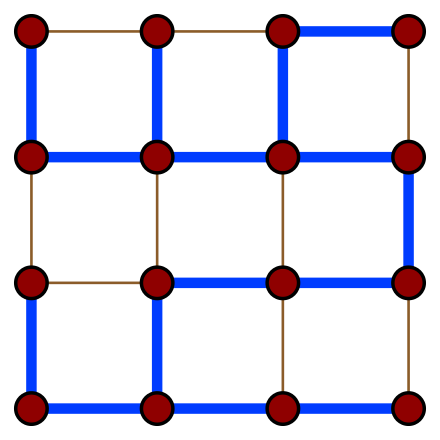
\includegraphics[scale=0.3]{img/spanning_tree.png}
          \caption{A spanning tree on a $4 \times 4$ grid graph. } 
          \label{fig:spanning_tree}
        \end{figure}
      \end{definition}

      Note that an unconnected graph will never have a spanning tree, but what about a connected graph? 

      \begin{theorem}[Spanning Trees of Connected Graphs]
        A connected graph will always have at least one spanning tree, not necessarily unique. 
      \end{theorem}

      Given a connected undirected weighted graph, we may want to find the \textbf{minimum spanning tree (MST)}, i.e. the spanning tree with edges $E^\prime$ such that the sum of the weights of all $e \in E^\prime$ is minimized.\footnote{An application of this is when we generally want to make sparse graphs. In a datacenter, wires can be expensive, so how I can minimize the length of wires to buy to construct a spanning subgraph?} How do we do this? There are two well-known algorithms to solve this. Prim's and Kruskal's algorithm.  
    
    \subsubsection{Prim's Algorithm with Cuts}

      Let's try to apply what we already know: Dijkstra. If we run Dijkstra on the graph starting at $s \in V$, we can get the shortest path from $s$ to every other node in the graph. This will give us a tree, but it may not be minimum. 

      \begin{figure}[H]
        \centering 
        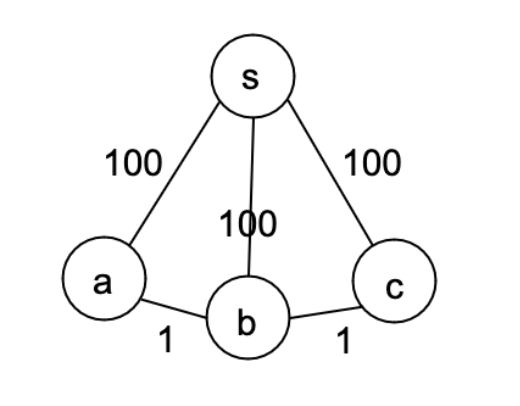
\includegraphics[scale=0.6]{img/dik_mst_prob.png}
        \caption{If we run Dijkstra on $s$, then our output will be a tree of cost $300$, even when the actual MST can be of cost $102$ starting from $a$.} 
        \label{fig:dik_mst_prob}
      \end{figure}

      It may seem like this is just a problem of where we start, but even this is not the case. 

      \begin{figure}[H]
        \centering 
        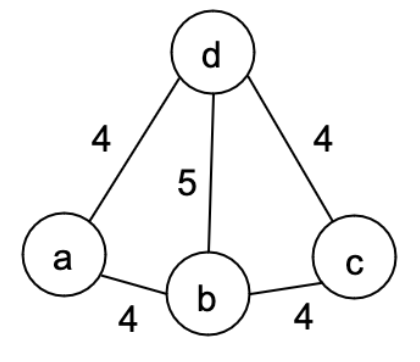
\includegraphics[scale=0.6]{img/dik_mst_prob2.png}
        \caption{No matter where we start from, we will never output the MST. The MST has cost $12$. If  we start from $b$ or $d$, we will get a tree of cost $13$. If we start from $a$ or $c$, we will get a tree of cost $16$.}
        \label{fig:dik_mst_prob2}
      \end{figure}

      \begin{definition}[Cuts]      
        Given graph $G(V, E)$, a \textbf{cut} is a partitioning of $V$ into $(S, V \setminus S)$. Furthermore, let $\mathrm{Cut}(S)$ be the number of edges with exactly one endpoint in $S$ and the other in $V \setminus S$. 
      \end{definition}

      \begin{theorem}[Cycles and Cuts]
        Given cycle $C \subset E$ in a graph and a cut $S \subset V$, 
        \begin{equation}
          | C \cap \mathrm{Cut}(S) | 
        \end{equation}
        is even. We can intuit this by visualizing the cycle as a long piece of looped string and a cut is a circle. The intersection between this circle and the string must be even since every time the cycle crosses through the cut, it must return back across the cut to the initial point.  
      \end{theorem}

      Now time for a bizarre theorem. 

      \begin{theorem}[Cut Property of MSTs]
        For all cuts $S \subset V$ of an undirected graph, the minimum cost edge in $\mathrm{Cut}(S)$ belongs to the MST. Furthermore, the converse is true: if we take all cuts and find all their minimum cost edges, these edges is precisely the MST! Therefore, an edge $e \in \mathrm{MST}$ iff $e$ is a min-cost edge for some cut. 
        \begin{figure}[H]
          \centering 
          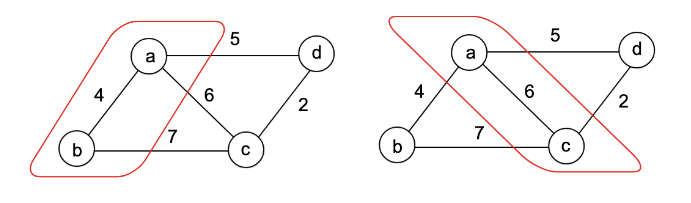
\includegraphics[scale=0.4]{img/mst_cut_prop.png}
          \caption{In the left cut, the edges are $(a,d), (b, c), (a, c)$. The minimum weight is $5$ on the $(a, d)$ edge, so it must be in the MST. For the right cut, $(c, d)$ must be in the MST. } 
          \label{fig:mst_cut_prop}
        \end{figure}
        The final part is that if we have all edge costs different, then we will have a \textit{unique} MST. 
      \end{theorem}
      \begin{proof}
        We use a greedy approach and prove by contradiction. Suppose that this is not true, i.e. there exists a cut $S$ with minimum cost edge $e$, and $e \not\in \mathrm{MST}$. Then, there exists some other edge $e^\prime \in \mathrm{Cut}(S)$ that is in the MST, since the MST is spanning and it must cross over to connect the whole graph. Well if we just put $e$ in and take $e^\prime$ out, we will still have a spanning tree since it connects the left spanning tree to the right spanning tree, and we now have a cheaper tree. So the original cannot be the MST in the first place. 

        To prove the converse, consider some edge $e$ in the MST and we must prove that it is the minimum cost edge in some cut. Note that if we take $e$ out, then it divides the MST into two connected components, and we can just define the cut as these subsets of nodes. So this is in $\mathrm{Cut}(S)$ for some $S \subset V$. We can also prove that this is minimal since if it wasn't the minimum cost edge for some cut, we could have taken it out and inserted a cheaper edge $e^\prime$ to begin with, getting a cheaper spanning tree.   
      \end{proof}

      We can just brute force this logic into an algorithm by going through all possible cuts and adding the minimum cost edge to our MST set. It is clear that a cut is defined by a subset of $S$, so really the number of cuts a graph can have is $2^{|S| - 1}$, which is exponential in $n$. However, the minimum spanning tree isn't exponential since it must have $n-1$ edges, so there must be many cuts with the same minimum edge. 

      One way is to start with one vertex $a$ that contains the minimum cost edge $(a, b)$ across all edges.  This edge must be minimal and must be in the MST. Then we can look at the cut $S = \{a, b\}$ and look at that cut. We keep doing this, keeping track of the set of edges we need to look at after adding a new node to our cut. So the number of cuts I consider is equal to the number of edges in the spanning tree.

      \begin{algo}[Prim's Algorithm to Find MST]
        It turns out that we can modify Dijkstra to solve it. 
        \begin{algorithm}[H]
          \label{alg:prim}
          \begin{algorithmic}[1]
            \Require{Graph $G(E, V)$}

            \Function{Prim}{s}
              \State $S \gets \{s\}$  \Comment{Our initial cut}
              \State $\pi[v] \gets$ list of size $|V|$ of $+\infty$ \Comment{$\pi[u]$ is min cost of getting from $u$ into the $S$}
              \State $\pi[v] = w_{sv}$ for all $v \in V$ \Comment{initialize list with neighboring nodes from start $s$}

              \While{$S \neq V$}
                \State $u = \mathrm{argmin}_{v \notin S} \pi[v]$ \Comment{Find node having minimum cost to reach from $S$}
                \State $S \gets S \cup \{u\}$ \Comment{Adding this node to $S$ to expand our cut}
                \For{$u \not\in S$} \Comment{Since we expanded $S$, our min reach distances}
                  \State $\pi[u] \gets \min\{\pi[u], w_{wu}\}$ \Comment{must be updated. It can only get shorter} 
                \EndFor \Comment{through a path from new $u$, so compare them}
              \EndWhile
              
            \EndFunction
          \end{algorithmic}
        \end{algorithm}

        \begin{figure}[H]
          \centering 
          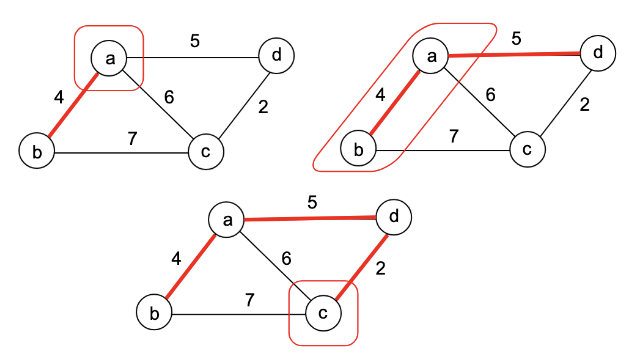
\includegraphics[scale=0.6]{img/prim.png}
          \caption{Step by step process of the method we mention above.} 
          \label{fig:prim}
        \end{figure}
        We are really going through two loops. We add to the cut $S$ $n$ times and for each time we add, we must compute the argmin, which is also $O(n)$, so our total time complexity of $O(n^2)$.  
      \end{algo}

      However, this is not efficient, so we can introduce a minheap to get the argmin step faster. 

      \begin{algo}[Prim's Algorithm with MinHeap]
        \begin{algorithm}[H]
          \label{alg:prims}
          \begin{algorithmic}[1]
            \Require{Nodes $V$, Edges $E$}
            \Function{Prim}{V, E}
              \State mst $\gets$ [] \Comment{Initialize mst array to return}
              \State s $\gets$ 0 \Comment{Choose any starting node}
              \State visited $\gets$ set() \Comment{Our expanding set of cuts.}
              \State edges $\gets$ minheap() \Comment{The set of low-weight edges that we can explore from}
              \State add (weight, s, next\_node) for edges in E \Comment{Look for edges from s to expand our cut from.}

              \While{|visited| < |V|} \Comment{Until we have visited all cuts,}
                \State weight, frm, to $\gets$ pop from edges \Comment{Get the cheapest edge to explore}
                \If{to $\not\in$ visited} \Comment{If this isn't already in our cut, }
                  \State add to $\rightarrow$ visited \Comment{Add it to our cut. From cut}
                  \State add (frm, to, weight) to mst \Comment{property, this must be added to mst}

                  \For{next\_to, next\_weight $\in$ E[to]} \Comment{After expanding, add newly discovered}
                    \If{next\_to $\not\in$ visited} \Comment{edges for future exploration}
                      \State push (next\_weight, to, next\_to) to edges
                    \EndIf
                  \EndFor
                \EndIf
              \EndWhile 

              \State \Return{mst} \Comment{of form (from, to, weight)}
            \EndFunction
          \end{algorithmic}
        \end{algorithm}

        You essentially push $n$ times and pop $m$ times, and the time per push and pop is $\log_2 (n)$. Therefore, the total time to push is $n \log(n)$ and to pop is $m \log (n)$, making the total runtime $O((n + m) log(n)) = O(m \log{n})$. 
      \end{algo}

      This can be sped up even faster if we use Fibonacci heaps or assume extra structure on the graph. 

    \subsubsection{Kruskal's Algorithm}

      If we were to try and construct this algorithm from scratch, we may take a greedy approach by incrementally adding the minimum cost edge from your cut. However, there is one thing to check: have we entered a cycle? Checking whether the next added node $a$ completes a cycle in $S \cup \{a\}$ is nontrivial. 

      \begin{theorem}[Cycle Property]
        For all cycles $C$, the max cost edge of $C$ does not belong to MST. 
      \end{theorem}

      Therefore, you can take $S$ and either add to it using the cut property or delete candidates from it using the cycle property. What is the best order to do this in? Kruskal's algorithm answers this question, which takes a greedy approach. 

      \begin{algo}[General Kruskal's Algorithm]
        The general idea is that we sort $e \in E$ in increasing cost, and for each $e \in E$, we use either the cut or cycle property to decide whether $e$ goes in or out. 

        \begin{algorithm}[H]
          \label{alg:prim_kruskal}
          \begin{algorithmic}[1]
            \Require{Graph $G(V, E)$}
            \Function{Kruskal}{V, E}
              \State sort $E$ in increasing cost 
              \State $T \gets \{\}$
              \For{$e \in E$}
                \If{$T \cup \{e\}$ does not have cycle} 
                  \State $T \gets T \cup \{e\}$ \Comment{Cut property}
                \Else \Comment{Cycle property} 
                  \State continue \Comment{discard $e$ since from sorting, this edge is heaviest in cycle}
                \EndIf
              \EndFor
            \EndFunction
          \end{algorithmic}
        \end{algorithm}

        \begin{figure}[H]
          \centering 
          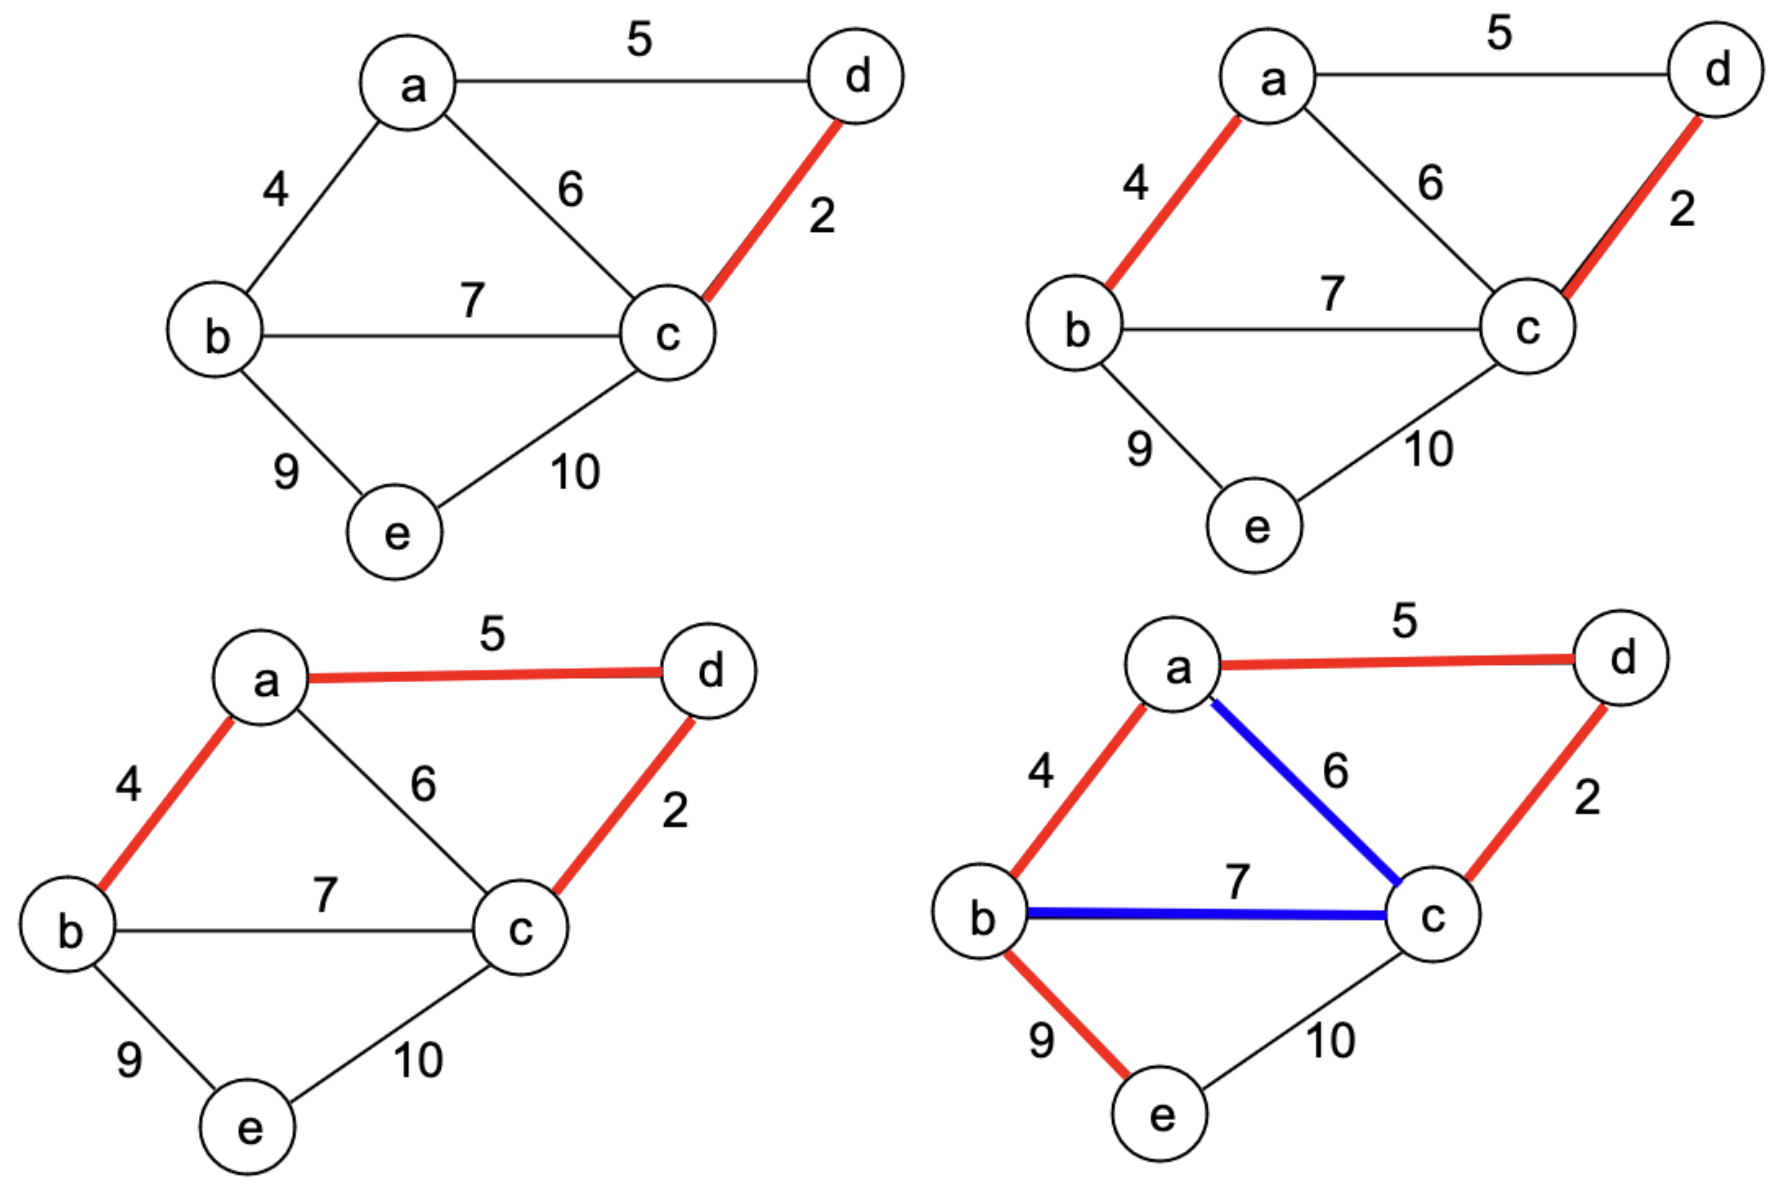
\includegraphics[scale=0.4]{img/kruskal.png}
          \caption{Kruskal's algorithm. In the last step, we see that the next minimum cost edge of 6 and 7 forms a cycle, so we add the edge of length 9.} 
          \label{fig:kruskal}
        \end{figure}
        The sorting of edges take $O(m \log{m})$ time, and after sorting, we iterate through all the edges and apply $m$ find-union algorithm, which each take at most $O(\log{n})$ time. Therefore, the overall complexity is $O(m \log{m} + m \log{n})$. However, the value of $m$ can be at most $O(n^2)$, so the two logarithms are essentially the same, arriving at the final runtime of $O(m \log{n})$. 
      \end{algo}

      The way to prove that this is correct is to show that every step you do is correct, known as \textit{structural induction}, either because of one of the two properties. Say that so far, we have some edges in $V$ which forms a partition of $V = \sqcup_i T_i$ of disjoint trees (can be trees, one edge, or just single nodes). We are looking at the next biggest edge $e = (a, b)$. There are two possibilities. 
      \begin{enumerate}
        \item If $a, b$ are both in a single $T_i$, then this forms a cycle and can be thrown away since this is the max cost edge in the cycle by the cycle property. 
        \item If $a, b$ connect $T_i$ and $T_j$ for $i \neq j$, then this edge is in $\mathrm{Cut}(T_i)$ and is the minimum cost edge since the rest of the edges in $\mathrm{Cut}(T_i)$ come next in the sorted $E$. Therefore this must be included by the cut property. 
      \end{enumerate}

      \begin{figure}[H]
        \centering 
        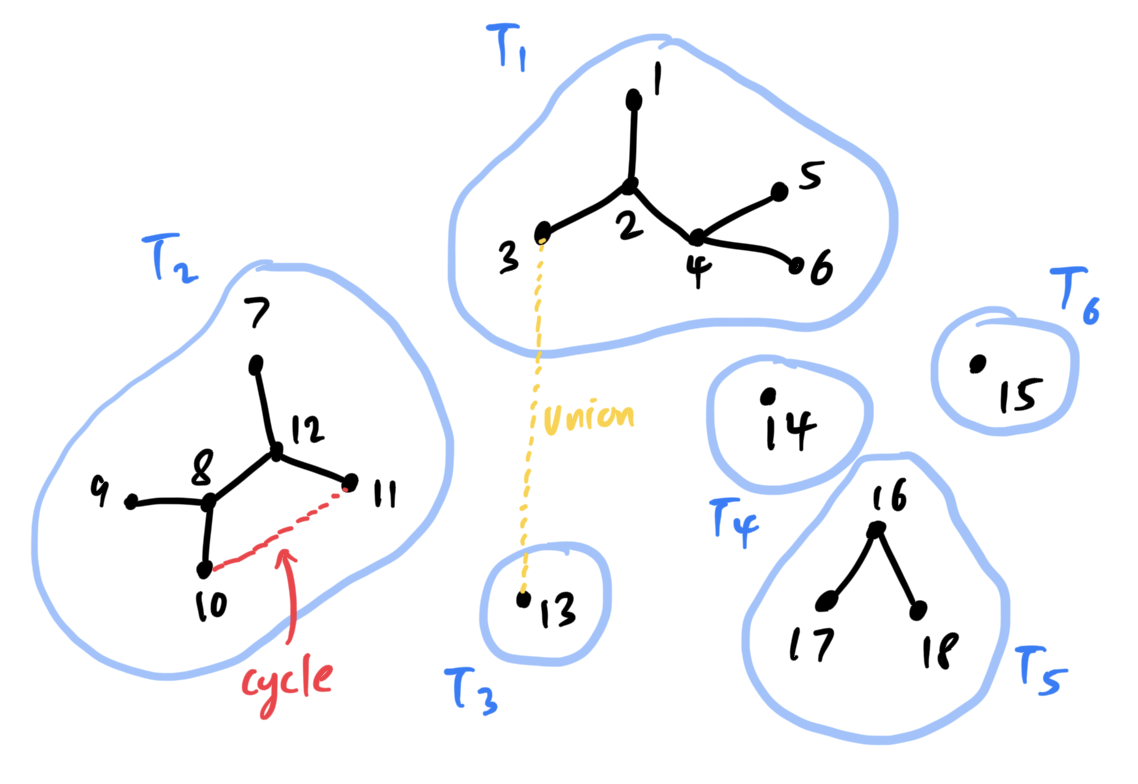
\includegraphics[scale=0.4]{img/sets.png}
        \caption{Each $T_i$ is a component formed by the edges chosen so far. For example, $T_1 = \{1, 2, 3, 4, 5, 6\}, \ldots$. We can either discard an edge (red) or include an edge (yellow). } 
        \label{fig:sets}
      \end{figure}

      The only bottleneck in here is line 5, where we check if $e$ does not complete a cycle in $T$. It will obviously not be efficient to do BFS, construct a tree, and see if there is a loop by checking if two points in the same layer are connected. It may help to decompose this algorithm into two steps: what is being stored and what is being checked? 

      Note that from our visual, we are really just keeping a set of these points that each make a subtree and connecting them together. How do we efficiently search for which cluster a point is a part of and efficiently merge two clusters? We could use a hashmap but this wouldn't work. We need something like a doubly linked list. 

      \begin{algo}[Kruskal's Algorithm]
        The implementation uses the Union-Find data structure. For clarity, we will not elaborate it but will show the full pseudocode. 
        \begin{algorithm}[H]
          \label{alg:kruskal}
          \begin{algorithmic}
            \Require{Nodes V. Edges $E = \{(u, v, w)\}$ where $u, v \in V$ and $w > 0$ is a weight. }
            \State 
            \Function{Kruskal}{V, E}
              \State $n \gets |V|$ 
              \State sort $E$ in increasing order of weights. \Comment{Needed for Kruskal}
              \State parent $\gets [0, \ldots, n-1]$ \Comment{Initialize the disjoint cluster each node is in}
              \State rank $\gets$ list of $0$s of size $n$ 

              \Function{Find}{x} 
                \If{parent[x] $\neq$ x} 
                \State parent[x] $\gets$ Find(parent[x]) \Comment{Path compression}
                \EndIf
                \State \Return{parent[x]}
              \EndFunction

              \Function{Union}{x, y} 
                \State px, py = find(x), find(y) 
                \If{px = py} 
                  \State \Return{False}
                \EndIf
                \If{rank[px] < rank[py]} 
                  \State parent[px] $\gets$ py
                \ElsIf{rank[px] > rank[py]}
                  \State parent[py] $\gets$ px
                \Else{}
                  \State parent[py] $\gets$ px 
                  \State rank[px] $\gets$ rank[px] + 1
                \EndIf
                \State \Return{True}
              \EndFunction

              \State mst $\gets$ [] 
              \For{u, v, weight $\in$ edges} 
                \If{union(u, v)} 
                  \State add (u, v, weight) to mst
                \EndIf 
                \If{len(mst) = n - 1}
                  \State break
                \EndIf 
              \EndFor

              \State \Return{mst}
            \EndFunction
          \end{algorithmic}
        \end{algorithm}
      \end{algo}
      
      To analyze the runtime of this, we define the function. 

      \begin{definition}[Ackerman Function]
        The \textbf{Ackerman function} is one of the fastest growing functions known. It is practically infinity. 
        \begin{equation}
          A(m,n) = 
          \begin{cases} 
            n+1 & \text{if } m = 0 \\
            A(m-1,1) & \text{if } m > 0 \text{ and } n = 0 \\
            A(m-1,A(m,n-1)) & \text{if } m > 0 \text{ and } n > 0
          \end{cases} 
        \end{equation}
        The inverse Ackerman function therefore grows extremely slowly. 
      \end{definition}

      If we optimize the steps in Kruskal's algorithm, we can get its runtime to 
      \begin{equation}
        O((m + n) \log^{\ast} (n))
      \end{equation}
      which is practically linear. 

    \subsubsection{Applications}

      Here is a way to cluster data, a surprising way to apply MSTs. It is the most widely used application, especially in data science. The problem is that given $n$ data points $x_i \in \mathbb{R}^d$ and an integer $k$, we want to partition the points into $k$ groups $\mathbf{C} = (C_1, \ldots, C_k)$ where $\mathbf{x} = \sqcup_i C_i$. You want to distances between the points within a group to be small and the distances between groups to be large. We can think of finding the objective which takes every pair of clusters and computes the minimum distance between these clusters, and we want to maximize this distance over all pairs of clusters.  

      \begin{algo}[Single Linkage/Hierarchical Clustering]
        The general idea is to take this dense graph, find the MST, and cut off the largest edges from this MST, which will give you $k$ components. This is the answer. Or really, you can use Kruskal's algorithm and terminate earlier when $T$ has $k$ sets/components. 
        Note that as we add edges as we construct our MST, we are merging two clusters into one. So that all you are doing is finding the next pair of closest points and merging the clusters that they are a part of. 

        \begin{algorithm}[H]
          \label{alg:clustering}
          \begin{algorithmic}[1]
            \Require{Nodes $V = \{v_i\} \subset \mathbb{R}^n$}
            \Function{Cluster}{V}
              \State Run Kruskal and at each iteration, check if you have $K$ clusters. 
              \State If so, terminate and return the \texttt{parent} list. 
            \EndFunction
          \end{algorithmic}
        \end{algorithm}
      \end{algo}

      \begin{theorem}
        The algorithm above minimizes the objective function. 
        \begin{equation}
          \argmax_{\mathbf{C}} \min_{p \in C_i, q \in C_j} \{ d(p, q) \}
        \end{equation}
      \end{theorem}
      \begin{proof}
        Let $\mathbf{C}^\ast$ be the MST clustering. We claim that for any other clustering $\mathbf{C} = \{C_1, \ldots, C_k\}$,  
        \begin{equation}
          \mathrm{min dist}(\mathbf{C}) \leq \mathrm{min dist}(\mathbf{C}^{\ast})
        \end{equation}
        Assume that this was not the case, so $\mathrm{min dist}(\mathbf{C}) > \mathrm{min dist}(\mathbf{C}^{\ast})$ and therefore there exists a $p, q \in C_i, C_j$ such that $d(p, q) = \mathrm{mindist}(\mathbf{C}) > \mathrm{min dist}(\mathbf{C}^\ast)$. Since this is a different clustering, $p, q$ must have been in the same cluster $C_i^\ast$. But note that since Kruskal adds edges in increasing length, all edges within a cluster must have length less edges that go across two clusters. 

        \begin{figure}[H]
          \centering 
          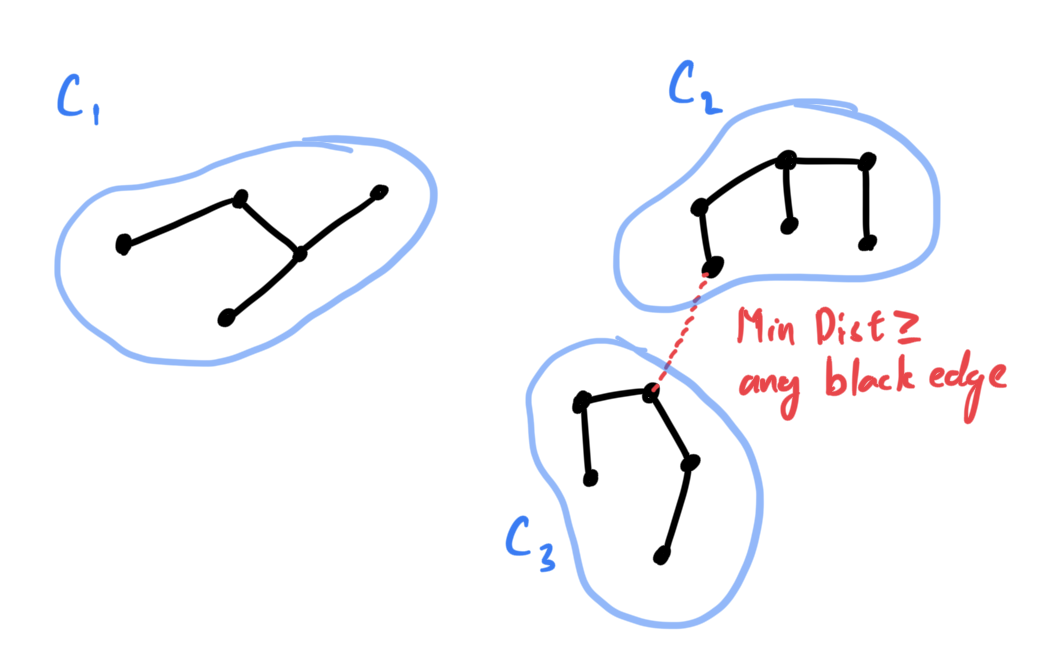
\includegraphics[scale=0.4]{img/mindist.png}
          \label{fig:mindist}
        \end{figure}

        So $d(p, q)$ must be the less than the length of all edges within a cluster in $\mathbf{C}^\ast$. But all within-cluster edges must be smaller than $\mathrm{min dist}(\mathbf{C}^\ast)$, meaning that $\mathrm{min dist}(\mathbf{C}^\ast) > d(p, q)$, contradicting the fact that is is greater, and we are done. 
      \end{proof}

      If you define the distance between two clusters to be the distance between the centroids (mean point), then this is called \textit{average linkage} (min avg distance). If we define the cluster distance as the maximum distance between two points, then it is called \textit{complete linkage} (min max distance). Kruskal's algorithm only worked for the single linkage case but may not work for these additional definitions. This is why there is usually a whole suite of clustering algorithms for a particular problem and we just find out which one fits the data the best. Furthermore, we have done \textit{bottom-up clustering}, where we took individual points to make clusters. In \textit{top-down clustering}, we take the whole set and cut it up into clusters.  

\section{Dynamic Programming}
  
    Let's take a look at a motivating example. 

    \begin{example}[Computing Fibonacci Numbers]
      To compute the $N$th Fibonacci number, we can use a recursive method. 
      \begin{algorithm}[H]
        \caption{}
        \label{alg:recfib}
        \begin{algorithmic}
          \Require{$N$}
          \State 
          \Function{RecFib}{$N$}
            \If{$N = 0$} 
              \State \Return{$0$}
            \ElsIf{$N = 1$}
              \State \Return{$1$}
            \Else 
              \State \Return{RecFib($N-1$) + RecFib($N-2$)}
            \EndIf
          \EndFunction
        \end{algorithmic}
      \end{algorithm}
    \end{example}

    This is exponential, in fact $O(\varphi^N)$ where $\varphi$ is the golden ratio. The reason is that we are repeatedly computing the same subproblem (e.g. RecFib($N-2$ is computed twice)), leading to inefficiency. It would be great if we could store these intermediate values rather than recomputing them. This introduces us to the concept of memoization. 

    \begin{definition}[Memoization]
      \textbf{Memoization} refers to storing intermediate values for reuse rather than computing them again (e.g. in future recursive calls). 
      
      Therefore, the term \textbf{dynamic programming} just means \textit{to deliberately evaluate and memoize in the correct order}. 
    \end{definition}


    \begin{algo}[Redursive Memoized Fibonacci]
      This leads us to a memoized version of computing Fibonacci Numbers, which is linear runtime. In fact, we can have constant space complexity since we don't need more than the last 2 previous Fibonacci numbers to compute the next one. 
      
      \begin{algorithm}[H]
        \caption{Memoized Fibonacci}
        \label{alg:memfib_rec}
        \begin{algorithmic}
          \Require{$N$}
          \State Initialize memo array $F[0..N]$ with -1
          \State $F[0] \gets 0$
          \State $F[1] \gets 1$
          \Function{MemFib}{$N$}
            \If{$N < 0$}
              \State \Return{$0$}
            \ElsIf{$F[N] \neq -1$}
              \State \Return{$F[N]$}
            \Else
              \State $F[N] \gets$ \Call{MemFib}{$N-1$} + \Call{MemFib}{$N-2$}
              \State \Return{$F[N]$}
            \EndIf
          \EndFunction
        \end{algorithmic}
      \end{algorithm}

      The runtime is computed, by taking the number of distinct problems (i.e. the number of calls to MemFib with distinct inputs) multiplied by the time per subproblem (constant since lookup is constant and adding is constant). Note that this assumes that arbitrary arithmetic operations take constant time, but this is not true if we look at the bit complexity, which can scale quite fast as these numbers grow. 
    \end{algo}

    Note that this does not really explicitly show the order in which the memoized list is being filled. It is implicit but hard to see in the recursive calls. Therefore, it may help to write it iteratively. 


    \begin{algo}[Iterative Memoized Fibonacci]
      In here, we can explicitly see that the $n$th Fibonacci number is explicitly dependent on the $n-2$ and $n-1$. 
      \begin{algorithm}[H]
        \caption{Iterative Fibonacci}
        \label{alg:iterfib}
        \begin{algorithmic}
          \Require{$N$}
          \State Initialize array $F[0..N]$
          \State $F[0] \gets 0$
          \State $F[1] \gets 1$
          \For{$i \gets 2$ to $N$}
            \State $F[i] \gets F[i-1] + F[i-2]$
          \EndFor
          \State \Return{$F[N]$}
        \end{algorithmic}
      \end{algorithm}
    \end{algo}

  \subsection{Longest Increasing Subsequence}

    \begin{definition}[Longest Increasing Subsequence]
      Given a sequence of numbers $A = \{a_1, a_2, ..., a_n\}$, a \textbf{longest increasing subsequence} is a subsequence $\{a_{i_1}, a_{i_2}, ..., a_{i_k}\}$ of $A$ such that:
      \begin{enumerate}
        \item $1 \leq i_1 < i_2 < ... < i_k \leq n$ (maintains original order)
        \item $a_{i_1} < a_{i_2} < ... < a_{i_k}$ (strictly increasing)
        \item $k$ is maximized (longest such subsequence)
      \end{enumerate}
    \end{definition}

    \begin{example}
      For the sequence $A = \{3, 10, 2, 1, 20, 4, 25\}$:
      \begin{itemize}
        \item $\{3, 10, 20, 25\}$ is an increasing subsequence of length 4
        \item $\{2, 4, 25\}$ is an increasing subsequence of length 3
        \item $\{3, 10, 20, 25\}$ is a longest increasing subsequence as no increasing subsequence of length 5 or greater exists
      \end{itemize}
    \end{example}

    For the actual problem of calculating the length of the LIS, dynamic programming gives us an efficient approach. First, let's do a brute force algorithm. 

    \begin{algo}[Recursive Brute Force LIS]
      At each step, we consider whether to include the current element in our subsequence. We can only include it if it's larger than the previous element we chose, maintaining the increasing property. We explore both possibilities (including and excluding) recursively to find the longest possible subsequence.
      \begin{algorithm}[H]
        \caption{Recursive Brute Force Longest Increasing Subsequence}
        \label{alg:reclis}
        \begin{algorithmic}
          \Require{Array $A[1..n]$}
          \Function{LIS}{$A, i, prev$}  \Comment{$i$ is current position, $prev$ is last element we took}
            \If{$i = n + 1$}  \Comment{If we've processed all elements}
              \State \Return{$0$}  \Comment{Return 0 as we can't add more elements}
            \EndIf

            \State // First choice: skip current element
            \State skip $\gets$ \Call{LIS}{$A, i+1, prev$}  \Comment{Keep same prev, move to next element}

            \State // Second choice: try to take current element
            \State take $\gets 0$  \Comment{Initialize take option to 0 in case we can't take it}
            \If{$A[i] > prev$}  \Comment{Only if current element maintains increasing sequence}
              \State take $\gets 1 +$ \Call{LIS}{$A, i+1, A[i]$}  \Comment{Add 1 for taking current element}
            \EndIf \Comment{Recursively find best sequence starting at i+1 with A[i] as previous}

            \State // Return best option between taking and skipping
            \State \Return{max(skip, take)}  \Comment{Choose the better of our two options}
          \EndFunction
          
          \State // Initial call with sentinel value to allow taking any first element
          \State \Return{\Call{LIS}{$A, 1, -\infty$}}  \Comment{Start at first element, no previous restrictions}
        \end{algorithmic}
      \end{algorithm}
      The runtime can be used by the recurrence relation. At every call, we may at most have to compute $2$ calls on the subarray not including the current element, and we compute the max of them which takes $O(1)$, so 
      \begin{equation}
        T(N) = 2 T(N-1) + O(1) \implies T(N) = O(2^N)
      \end{equation}
      which is not good. 
    \end{algo}

    Now let's move to our DP solution. 

    \begin{algo}[Dynamic Programming LIS]
      The key insight is that LIS[i] (the length of the LIS within the input array ending at i, inclusive) depends on all previous LIS[j] where j < i and A[j] < A[i]. For each position i, we can extend any previous increasing subsequence that ends with a smaller value. In other words, we are solving 
      \begin{equation}
        \mathrm{LIS}[i] = 1 + \max\{\mathrm{LIS}[j] \mid j < i \text{ and } A[i] > A[j] \}
      \end{equation}

      \begin{algorithm}[H]
        \caption{Dynamic Programming Longest Increasing Subsequence}
        \label{alg:dplis}
        \begin{algorithmic}
          \Require{Array $A[1..n]$}
          \Function{DPLIS}{$A$}
            \State // Initialize LIS array - each single element is an increasing sequence
            \State Initialize array $LIS[1..n]$ with $1$  \Comment{Base case: each element forms LIS of length 1}
            
            \For{$i \gets 2$ to $n$}  \Comment{Consider each element as end of sequence}
              \For{$j \gets 1$ to $i-1$}  \Comment{Look at all previous elements}
                \If{$A[i] > A[j]$}  \Comment{Can we extend sequence ending at j?}
                  \State $LIS[i] \gets \max(LIS[i], LIS[j] + 1)$  \Comment{Take best possible extension}
                \EndIf
              \EndFor
            \EndFor
            
            \State \Return{LIS[-1]} \Comment{Find the maximum value in LIS array}
          \EndFunction
        \end{algorithmic}
      \end{algorithm}

      The runtime is $O(n^2)$ since we have two nested loops, and the space complexity is $O(n)$ since we store one value for each position in the array. Note that we could also have filled this DP array backwards by considering all arrays that start at $A[i]$. 
    \end{algo}

    \begin{example}[DPLIS for Small Array]
      For array $A = [3,1,4,1,5]$:
      \begin{itemize}
        \item Initially: $LIS = [1,1,1,1,1]$
        \item After processing $i=2$: $LIS = [1,1,1,1,1]$
        \item After $i=3$: $LIS = [1,1,2,1,1]$ (4 can extend sequence from 3)
        \item After $i=4$: $LIS = [1,1,2,2,1]$
        \item After $i=5$: $LIS = [1,1,2,2,3]$ (5 can extend sequence from 4)
      \end{itemize}
      Final answer is 3, corresponding to subsequence $[3,4,5]$
    \end{example}

  \subsection{0/1 Knapsack} 

    Another application of DP is in the following problem. 

    \begin{definition}[0/1 Knapsack]
      Given a knapsack with maximum weight capacity $W$, along with a set of $n$ items, each with:
      \begin{itemize}
        \item Weight/Cost $c_i$
        \item Value $v_i$
      \end{itemize}
      You want to know the size of the subset of items that maximizes total value while keeping total weight/Cost $\leq W$. The constraint is that each item can be picked at most once (hence 0/1). 
    \end{definition}

    \begin{example}
      For $n = 3$ items and capacity $W = 4$:
      \begin{itemize}
        \item Item 1: $(c_1 = 2, v_1 = 3)$
        \item Item 2: $(c_2 = 1, v_2 = 2)$
        \item Item 3: $(c_3 = 3, v_3 = 4)$
      \end{itemize}
      Optimal solution: Take items 1 and 2
      \begin{itemize}
        \item Total weight: $2 + 1 = 3 \leq 4$
        \item Total value: $3 + 2 = 5$ (maximum possible)
      \end{itemize}
    \end{example}

    The most natural way to approach this would be greedy, but this does not exactly work. 

    \begin{example}[Counter-Example for Greedy Knapsack]
      Let's consider a knapsack with capacity $W = 10$ and:
      \begin{itemize}
        \item Values $V = [100, 48, 60, 11]$
        \item Weights $C = [10, 6, 4, 1]$
      \end{itemize}
      Then the value/weight ratios would be 
      \begin{equation}
        V/C = [10, 8, 15, 11]
      \end{equation}
      and so we would choose to gain 60 for cost 4, then gain 11 for cost of 1. We do not have enough to buy any more and have a cost of 71, when we could have gotten a cost of 108 by buying 60 and 48 for a total of 10. 
    \end{example}

    Just like as always, we just solve this using recursive brute force and then apply optimization with DP. 

    \begin{algo}[Recursive Brute Force Knapsack]
      The key idea is that for each item, we have two choices: either include it (if we have enough capacity) or exclude it. We try both possibilities recursively to find the maximum value possible. In here, $i$ represents the current item we're considering and $r$ is the remaining weight we can still use. 
      \begin{algorithm}[H]
        \caption{Recursive Knapsack}
        \label{alg:recknapG}
        \begin{algorithmic}
          \Require{Values $V[1..n]$, Weights $W[1..n]$, Capacity $C$}
          \State V, W
          \Function{Knapsack}{$i, r$}  
            \If{$i = n + 1$ or $r = 0$}  \Comment{Base case}
              \State \Return{$0$}   \Comment{Either we've considered all items or filled the knapsack}
            \EndIf \Comment{No more value can be added}

            \State skip $\gets$ \Call{Knapsack}{$i+1, r$}  \Comment{1st Op: Skip current item and maintain same $r$}

            \State take $\gets 0$  \Comment{2nd Op: Try to include curr item}
            \If{$W[i] \leq r$}  \Comment{Only try taking if item's weight fits in remaining $r$}
              \State take $\gets V[i] +$ \Call{Knapsack}{$i+1, r - W[i]$} \Comment{Add current item's value + best value from remaining items}
            \EndIf \Comment{Subtract current item's weight from remaining $r$}

            \State \Return{$\max(take,skip)$} \Comment{Return best possible value between two choices}
          \EndFunction
          
          \State // Start considering from first item with full $r$ 
          \State \Return{\Call{Knapsack}{$1, C$}}
        \end{algorithmic}
      \end{algorithm}
    \end{algo}

    Now let's apply memoization. 

    \begin{algo}[Dynamic Programming Knapsack]
      The key insight is that $K[i,r]$ (best value possible using items up to i exclusive with remaining capacity r) can be built from $K[i-1,r]$ and $K[i-1,r-W[i]]$ using the formula 
      \begin{equation}
        K[i,r] = \begin{cases}
          K[i-1,r] & \text{if } W[i] > r \text{ (can't take item i)} \\
          \max(K[i-1,r], V[i] + K[i-1,r-W[i]]) & \text{if } W[i] \leq r \text{ (can take item i)}
        \end{cases}        
      \end{equation}
      In here, i represents the items 1..i we're considering and r represents the remaining capacity.
      \begin{algorithm}[H]
        \caption{Dynamic Programming Knapsack}
        \label{alg:dpknap}
        \begin{algorithmic}
          \Require{Values $V[1..n]$, Weights $W[1..n]$, Capacity $C$}
          \State V, W
          \Function{DPKnapsack}{$C$}
            \State Create table $K[0..n, 0..C]$ \Comment{K[i,r] = max value using items V[:i] with remaining r}
            \State Initialize all entries to 0
            
            \For{$i \gets 1$ to $n$}  \Comment{Consider each item}
              \For{$r \gets 0$ to $C$}  \Comment{Consider each possible remaining capacity}
                \State $K[i,r] \gets K[i-1,r]$  \Comment{Default: inherit value from excluding item i}
                \If{$r \geq W[i]$}  \Comment{If current item fits in remaining capacity}
                  \State take $\gets V[i] + K[i-1,r-W[i]]$  \Comment{Value of item i + best value with remaining r}
                  \State $K[i,r] \gets \max(K[i,r],$ take$)$  \Comment{Take better of including or excluding}
                \EndIf
              \EndFor
            \EndFor
            
            \State \Return{$K[n,C]$}  \Comment{Best value possible using all items}
          \EndFunction
        \end{algorithmic}
      \end{algorithm}
      The memory complexity is obviously $\Theta(n C)$. The number of subproblems is $nC$, and the processing for each step is constant time (possibly addition and max), so $O(1)$. Therefore the total runtime is $O(nC)$ also. Note that if we compare this in terms of the bit runtime, then this is $O(n \log_2 C)$, which is psuedopolynomial since $C$ is described by $\log_2 {C}$ bits. However, the $n$ will scale linearly since it is the size of the array and not the size of each integer in $V, W$. 
    \end{algo}

    Note that if $C$ can be very big, and this can be problematic. 

  \subsection{Line Breaking}

    \begin{definition}[Line Breaking]
      Line breaking is used whenever you compile a tex document. Given 
      \begin{itemize}
        \item a sequence of words $w_1, w_2, ..., w_n$ where $w_i$ has length $l_i$
        \item a maximum line length $L$
        \item each line must contain whole words in order, separated by spaces
      \end{itemize}
      Our goal is to break words into lines to minimize the sum of squares of empty spaces at the end of each line, i.e. our cost function for a sequence of words $W[i:j+1]$ is 
      \begin{equation}
        \bigg( L - \sum_{k=i}^j w_k \bigg)^2
      \end{equation} 
      If we used the absolute value, there exists a greedy solution. 
    \end{definition}

    \begin{example}[Line Breaking Example]
      Given $L = 20$ and $W = [12, 8, 9]$ (note that spaces won't count in length in this problem), we have 3 possible arrangements. 
      \begin{enumerate}
        \item Option 1: First two words on first line
        \begin{itemize}
          \item Line 1: [12 + 8 = 20] (0 spaces remain)
          \item Line 2: [9] (11 spaces remain)
          \item Total cost = $0^2 + 11^2 = 121$
        \end{itemize}

        \item Option 2: Words one per line
        \begin{itemize}
          \item Line 1: [12] (8 spaces remain)
          \item Line 2: [8] (12 spaces remain)
          \item Line 3: [9] (11 spaces remain)
          \item Total cost = $8^2 + 12^2 + 11^2 = 64 + 144 + 121 = 329$
        \end{itemize}

        \item Option 3: Word 2 and 3 together
        \begin{itemize}
          \item Line 1: [12] (8 spaces remain)
          \item Line 2: [8 + 9 = 17] (3 spaces remain)
          \item Total cost = $8^2 + 3^2 = 64 + 9 = 73$
        \end{itemize}
      \end{enumerate}
      Therefore, Option 3 is optimal with cost 73. This also demonstrates that the greedy strategy, which gives Option 1, will not work. 
    \end{example}

    We start off with recursive brute force. Given any word $w_i$, we can either end the line there $w_i |$ or add another word $w_i w_{i+1}$. 

    \begin{algo}[Recursive Brute Force Line Breaking]
      The key idea is at each position i, we try placing different numbers of words on the current line and recursively solve for the rest. For each word i, we try all possible ways to break the line starting at word i. Let $MinCost(i)$ be the minimum cost to arrange words $[i..n]$. Then:
      \begin{equation}
        MinCost(i) = 
        \begin{cases}
          0 & \text{if } i > n \\
          \min_{i \leq j \leq n} \big\{ (L - \sum_{k=i}^j W[k])^2 + MinCost(j+1) \big\} & \text{if else} 
        \end{cases}
      \end{equation}
      where $(L - \sum_{k=i}^j W[k])^2$ is the cost to put the words $i...j$ on a new line and then ending. So whenever we add the new $i$th word at the end of the line, we are looking at all words $j$ at which we can break the line, and taking the minimum cost given this line break. The line break from $j+1$ should be computed as well (this is what we will store in our DP array later). 

      \begin{algorithm}[H]
        \caption{Recursive Line Breaking}
        \label{alg:recline}
        \begin{algorithmic}
          \Require{Word lengths $W[1..n]$, Line length $L$}
          \State W
          \Function{MinCost}{$i$}  \Comment{Returns min cost for words[i..n]}
            \If{$i = n + 1$}  \Comment{Base case: no words left}
              \State \Return{$0$}
            \EndIf

            \State min\_cost $\gets \infty$
            \State lineLen $\gets 0$
            \For{$j \gets i$ to $n$}  \Comment{Try placing words i through j on current line}
              \State lineLen $\gets$ lineLen $+ W[j]$
              \If{lineLen $\leq L$}  \Comment{If these words fit on the line}
                \State spaces $\gets L -$ lineLen  \Comment{Extra spaces at end of line}
                \State cost $\gets$ spaces$^2 +$ \Call{MinCost}{$j+1$}  \Comment{Cost of this line + rest}
                \State min\_cost $\gets \min($min\_cost$,$ cost$)$
              \EndIf
            \EndFor
            \State \Return{min\_cost}
          \EndFunction
          
          \State \Return{\Call{MinCost}{$1$}}  \Comment{Start with first word}
        \end{algorithmic}
      \end{algorithm}
    \end{algo}

    \begin{example}[Recursive Brute Force Line Breaking]
      For example, with $L=20$ and $W=[12,8,9]$:
      \begin{itemize}
        \item At $i=1$: Try
          \begin{itemize}
            \item [12] alone (8 spaces) + solve for [8,9]
            \item [12,8] together (0 spaces) + solve for [9]
          \end{itemize}
        \item At $i=2$: Try
          \begin{itemize}
            \item [8] alone (12 spaces) + solve for [9]
            \item [8,9] together (3 spaces) + solve for []
          \end{itemize}
        \item At $i=3$: Try
          \begin{itemize}
            \item [9] alone (11 spaces) + solve for []
          \end{itemize}
      \end{itemize}
    \end{example}

    \begin{algo}[Dynamic Programming Line Breaking]
      The key insight is that $DP[i]$ represents the minimum cost of optimally arranging words $[i..n]$. For each word i, we try placing words $[i..j]$ on a line and add the cost of optimally arranging the remaining words $[j+1..n]$. We do the same logic but rather than computing it we just retreive it from the DP array. 

      \begin{equation}
        DP[i] = 
        \begin{cases}
          0 & \text{if } i > n \\
          \min_{i \leq j \leq n} \big\{ (L - \sum_{k=i}^j W[k])^2 + DP[j+1] \big\} & \text{if else} 
        \end{cases}
      \end{equation}


      \begin{algorithm}[H]
        \caption{Dynamic Programming Line Breaking}
        \label{alg:dpline}
        \begin{algorithmic}
          \Require{Word lengths $W[1..n]$, Line length $L$}
          \State W
          \Function{LineBreak}{$L$}
            \State Create array $DP[0..n]$ \Comment{DP[i] = min cost for words[i..n]}
            \State Initialize all entries to $\infty$
            \State $DP[n+1] \gets 0$ \Comment{Base case: no words left}
            
            \For{$i \gets n$ downto $1$}  \Comment{Consider each starting word}
              \State lineLen $\gets 0$
              \For{$j \gets i$ to $n$}  \Comment{Try placing words i through j on a line}
                \State lineLen $\gets$ lineLen $+ W[j]$
                \If{lineLen $\leq L$}  \Comment{If these words fit on the line}
                  \State spaces $\gets L -$ lineLen \Comment{Extra spaces at end}
                  \State cost $\gets$ spaces$^2 + DP[j+1]$ \Comment{Cost of this line + rest}
                  \State $DP[i] \gets \min(DP[i],$ cost$)$ \Comment{Update if better}
                \EndIf
              \EndFor
            \EndFor
            
            \State \Return{$DP[1]$}  \Comment{Cost of optimally arranging all words}
          \EndFunction
        \end{algorithmic}
      \end{algorithm}

      The memory complexity is clearly $O(n)$. To add each element $i$, we must iterate over all the possible $j$'s, making this $O(n^2)$ total iterations. However, computing the cost is also $O(n)$, making the total runtime $O(n^3)$. However, if we also store another DP array \texttt{sums}, which can be computed in linear time and stores 
      \begin{equation}
        \texttt{sums}[i] = \sum_{k=i}^n w_k \implies \sum_{k=i}^{j}  = \sum_{k=i}^n w_k - a\sum_{k=j+1}^n w_k = \texttt{sums[i]} - \texttt{sums[j+1]}
      \end{equation}
      which can be accessed and computed in $O(1)$ time, bringing us down to $O(n^2)$. 
    \end{algo}

    \begin{example}[DP Line Breaking]
      For example, with $L=20$ and $W=[12,8,9]$:
      \begin{itemize}
        \item $DP[4] = 0$ (base case)
        \item $DP[3] = 11^2 = 121$ (only option for last word)
        \item $DP[2] = \min(12^2 + 121, 3^2) = \min(265, 9) = 9$ (alone or with word 3)
        \item $DP[1] = \min(8^2 + 9, 0^2 + 121) = \min(73, 121) = 73$ (alone or with word 2)
      \end{itemize}
    \end{example}

  \subsection{Bellman Ford Revisited} 

    Recall the Bellman equations that we must solve using DP. That is, given some $s \in V$, 
    \begin{equation}
      d[v] = \min_w \{ d[w] + l_{wv} \}
    \end{equation}
    with $d[s] = 0$. Note that the problem was not well defined if there are negative cycles in the graph, since we can just loop an infinite number of times. However, we can modify the bellman equations to get a better sense. 

    \begin{theorem}[Modified Bellman Equations]
      For paths of length at most $i$ edges, the Bellman equations become:
      \begin{align}
        d(v,i) = \begin{cases} 
          0 & \text{ if } v = s \\
          \min\{d(v,i-1), \min_{(u, v) \in E} \{d(u,i-1) + w_{uv}\}\} & \text{ otherwise}
        \end{cases}
      \end{align}
      where $d(v,i)$ represents the shortest path from source $s$ to vertex $v$ using at most $i$ edges, and $w_{uv}$ represents the weight of edge $(u, v)$. Note that the inner minimum takes the minimum over all paths with the final edge connecting from some other node $u$ to target $v$, and the outer minimum compares this minimum path to what we already have to see if it's an improvement. 
    \end{theorem} 

    This indicates that we should use a 2D DP array to memoize. This allows you to have a more flexible representation in case there are negative cycles since we are also limiting the number of edges a path could have. 

    \begin{algo}[2D DP Bellman-Ford]
      The implementation of the modified equations gives us the following algorithm. 
      \begin{algorithm}[H]
        \label{alg:bellman_ford_leq}
        \begin{algorithmic}[1]
          \Require{Nodes $V$, Edges $E$, source $s$}
          \State $d \gets$ 2D array of size $|V| \times |V|$ initialized to $\infty$
          \State $d[s,0] \gets 0$ \Comment{Base case: Can reach source with 0 edges}
          
          \For{$i = 1, \ldots, n-1$}
            \For{$v \in V$}
              \State $d[v,i] \gets d[v,i-1]$ \Comment{Keep best path seen so far}
              \For{$(u,v) \in E$}
                \State $d[v,i] \gets \min(d[v,i], d[u,i-1] + l_{uv})$
              \EndFor
            \EndFor
          \EndFor
        \end{algorithmic}
      \end{algorithm}
      Note that this algorithm still has time complexity $O(nm)$ because the outer loop runs $n-1$ times and for each iteration, we examine each edge once. The space complexity is $O(n^2)$, and finally, note the important properties. 
      \begin{enumerate}
        \item \textit{Monotonicity}: For all vertices $v$ and indices $i$:
        \begin{equation}
          d(v,i) \leq d(v,i-1)
        \end{equation}
        This is because any path using $\leq (i-1)$ edges is also a valid path using $\leq i$ edges.

        \item \textit{Convergence}: The algorithm will stabilize after at most $n-1$ iterations since:
        \begin{itemize}
          \item Any shortest path without negative cycles can use at most $n-1$ edges
          \item Therefore, $d(v,n-1) = d(v,n)$ for all $v$ if no negative cycles exist
        \end{itemize}

        \item \textit{Negative Cycle Detection}: A negative cycle exists if and only if:
        \begin{equation}
          \exists v \in V : d(v,n) < d(v,n-1)
        \end{equation}
        This is because any improvement after $n-1$ edges must use a negative cycle.
      \end{enumerate}
    \end{algo}

\section{Hashing and Probabilistic Algorithms} 

  One of the most important applications of hashing and probabilistic algorithms is in cryptography. For example, when you generate a RSA keypair, you must choose two 128-bit prime numbers which serve as your private key. State of the art methods simply generate a random 128-bit prime number perform \textit{independent} randomized probabilistic tests with error rate $\epsilon$. Given that this is independent, simply running this tests $k$ times reduces our error exponentially to $\epsilon^k$, practically guaranteeing primality. In Bitcoin and Ethereum wallets, hardened child key derivation functions in hierarchical determinstic wallets hash subsets of the parent key to generate both the child keys and their seeds.\footnote{For an implementation of both, look at my blockchain implementation \href{https://github.com/mbahng/blade/blob/main/backend/src/crypt/primes.js\#L61}{here}} 

  \subsection{Hashing} 

    Assume we want to map keys from some \textbf{universe} $U$ into a smaller set $[N] = \{1, \ldots, N\}$ of $N$ bins. The algorithm will have to handle some dataset $S \subset U$ of $|S| = M$ keys.\footnote{For example, think of all possible strings as $U$ and all $256$-bit numbers as $N = 2^{256}$. $S$ in this case $S$ may be the set of all addresses on a blockchain. This is SHA256, and to date there is no known hash collisions, though there are a few for SHA1.} We want to store $S$ with efficient performance in 
    \begin{enumerate}
      \item \texttt{Find(x)}, which returns true if $x \in S$
      \item \texttt{Insert(x)} 
      \item \texttt{Delete(x)}
      \end{enumerate}
    This is essentially a set. If one is new to hashing, we could try to use a balanced binary search tree or a heap (implemented as a red-black tree or some other variant), which can do all three operations in $O(\log(N))$ time. If we had access to a randomized function $h: U \rightarrow [N]$, with the property that for a fixed $x \in U$, $h(x) \sim \mathrm{Multinomial}(N)$, then by linearity of expectation\footnote{Note that this is not $\mathbb{P}_{x, y}$ since $x, y$ are not random variables. They are fixed, and $h(x), h(y)$ are the random variables. }
    \begin{equation}
      \mathbb{P}(h(x) = h(y)) = \mathbb{E}[\mathbbm{1}_{h(x) = h(y)}] = \frac{N}{N^2} = \frac{1}{N}
    \end{equation}
    This is great, but this is also random, which means that we are not guaranteed to map to the same bin across time. If we add time-invariance, this is pretty much a hash function, which is really deterministic, but we like to call it psuedo-random. 

    So what if there are collisions? They are inevitable anyways even with a completely random function, but minimizing them will give us the best runtime performance. There are a two main ways to approach this. 
    \begin{enumerate}
      \item At each bin, store the head of a linked list, BST, or another hash table. You would incur an additional linear, logarithmic, or constant cost of traversing this data structure for each operation.  
      \item Look for another bin. We can just look at $h(x) + 1$ or $h(h(x))$ (or really any deterministic function $f(h(x))$) if $h(x)$ is occupied. 
    \end{enumerate}

    This is what we have to work with here, so we would like to modify our assumptions. Therefore, we can achieve good performance by reducing the collisions and by improving how we deal with collisions. We will focus on the first part, and we would like for our hash functions to have some nice properties, which we will define. The most intuitive way is to treat $x, y$ as random variables uniformly sampled from $U$, and then we would like $\mathbb{P}(h(x) = H(y)) \approx 1/N$. However in practice, this is not the case since our subdomain $S$ is already fixed, yet may be unknown. Therefore given any function $h$, we can construct an adversarial sequences of inputs that will all map to the same bin. We must therefore consider a \textit{family} of hash functions. 

    \begin{definition}[Universal Hashing]
      A family of hash functions $H = \{h : U \rightarrow [N] \}$ is \textbf{universal} if for any fixed $x, y \in U$, 
      \begin{equation}
        \mathbb{P}_{h} \big( h(x) = h(y) \big) \leq \frac{1}{N}
      \end{equation}
      where $h$ is drawn uniformly. If the bound is $2/N$ then it is called \textbf{near-universal}, and what's important is the $N$ in the denominator. This polynomial decay in collision probabilities is exactly what we need for constant operation time. That is, given query $x$, let the random variable $X$ be the number of operations we must do to find $X$, which consists of $1$ pointer traversal plus some other amount of traversals (e.g. through a linked list) if collision, say which is $C_n$. So we have 
      \begin{equation}
        X = 1 + \sum_{y \in S} Q_y
      \end{equation}
      where $1$ comes from the initial pointer traversal in hashing, and Bernoulli $Q_y = 1$ if $h(y) = h(x)$.\footnote{This may not be $1$ since we may have to do more than 1 additional traversal, e.g. in linked lists. But we assume the extra cost is bounded by a constant.} Then, by linearity of expectation combined with the bound on probability of collision we have 
      \begin{equation}
        \mathbb{E}[X] = 1 + \sum_{y \in S} \mathbb{E}[Q_y] = 1 + |S| \cdot \mathbb{P}(h(x) = h(y)) = 1 + \frac{|S|}{N}
      \end{equation} 
      which is constant. 
    \end{definition} 

    If $H$ is the set of all functions from $U$ to $[N]$, then this universal property is trivially satisfied since 
    \begin{equation}
        \mathbb{P}_{h} \big( h(x) = h(y) \big) = \frac{1}{N}
    \end{equation}
    But this is quite a complex function class and $h$ may not be easy to store, i.e. may not be analytic. The question now becomes whether we can achieve universality with a smaller class. It turns out yes, and the obvious use is to use cyclic groups. 

    \begin{lemma}[Carter-Wegman 71]
      Suppose $U = \{0, 1, \ldots, M-1\}$. We choose a prime $p \geq M$\footnote{It is guaranteed that a prime exists between $m$ and $2m$.} and construct the family 
      \begin{equation}
        H = \{h_a (x) = (ax \mathrm{ mod } p ) \mathrm{ mod } N \mid a = 0, \ldots, p-1 \}
      \end{equation}
      We claim this is near-universal. 
    \end{lemma}
    \begin{proof}
      We treat $x$ as the generator of this group, and then $ax \mathrm{ mod } p = a^\prime x { mod } p$ iff $a = a^\prime$. Therefore, 
      \begin{equation}
        \mathbb{P}_a (h_a (x) = h_a (y)) = \mathbb{P}_a \big( (ax - ay) \mathrm{ mod } p = N k \big)
      \end{equation}
      for some $k$. If $a = 0$, then everything collides, but if $a \neq 0$ and $x \neq y$, then $ax - ay$ must have a difference of exactly a multiply of $N$, which happens with probability $1/N$. Therefore, we have 
      \begin{equation}
        \mathbb{P}_a (h_a (x) = h_a (y)) = \mathbb{P}(a = 0) + \mathbb{P}(a \neq 0) \cdot \frac{1}{N} = \frac{1}{p} + \frac{p-1}{p} \cdot \frac{1}{N} < \frac{2}{N} 
      \end{equation}
      since $p > N$. 
    \end{proof}

    Therefore, to hash, 
    \begin{enumerate}
      \item we choose a prime $p \geq m = |U|$. 
      \item choose $a \in \{0, 1, \ldots, p-1\}$ at random. 
      \item Use $h_a(x) = (ax \mathrm{ mod } p ) \mathrm{ mod } N$ to hash everything.\footnote{We do not change $a$ every time we hash. }
    \end{enumerate}

    \begin{example}
      Let $n$ be a fixed prime number and 
      \begin{equation}
        H = \{h_{a, b} (x, y) = ax + by \mathrm{ mod } n : a, b \in [n] \}
      \end{equation} 
      We claim that this is universal. Let $x = (x_1, x_2)$ and $y = (y_1, y_2)$ be arbitrary pairs of integers where $x \neq y$. WLOG, assume $x_2 \neq y_2$. Then 
      \begin{equation}
        \mathbb{P}(h_{a, b} (x) = h_{a, b} (y)) = \mathbb{P}(a x_1 + b x_2 = a y_1 + b y_2) = \mathbb{P}\big( a (x_1 - y_1) = b (y_2 - x_2) \big)
      \end{equation} 
      Suppose that we pick $a$ first and we compute the conditional probability. Then the LHS is a constant, and for this to hold in a cyclic group, $b$ must equal $c (y_2 - x_2)^{-1}$, which occurs with probability $1/N$. Using LOTP the joint probability is also $1/N$. 
    \end{example}

  \subsection{Modulo Operations}

  \subsection{Primality Testing}

\section{Flows and Cuts} 

  \subsection{Max-Flow Min-Cut Theorem} 

    \begin{definition}[Flow Network]
      Given a nonnegative weighted directed graph $G(V, E)$, we can define the weights to be the \textbf{capacity} $C: E \rightarrow \mathbb{R}^+$ of some commodity that can travel through the edge. Say that we have a source node $s \in V$ and a sink/destination node $t \in V$. This is called a \textbf{flow network}.
    \end{definition}

    \begin{definition}[Flow]
      Given a flow network, a \textbf{flow} is a function $f: E \rightarrow \mathbb{R}^+$ satisfying 
      \begin{enumerate}
        \item \textit{Conservation}. What flows in must always flow out. For all $v \neq s, t$, we have 
          \begin{equation}
            \sum_{(u \rightarrow v) \in E} f(u \rightarrow v) = \sum_{(v \rightarrow w) \in E} f(v \rightarrow w)
          \end{equation}

        \item \textit{Feasibility}. We cannot exceed the capacity. For all $e \in E$, 
          \begin{equation}
            0 \leq f(e) \leq C(e)
          \end{equation}
      \end{enumerate}
      The \textbf{value} of a flow represents the actual/realized amount of the commodity that we can push through the graph
      \begin{equation}
        |f| = \sum_{(s \rightarrow u) \in E}  f(s \rightarrow u) - \sum_{(u \rightarrow s) \in E}  f(u \rightarrow s) 
      \end{equation} 
      where we need to subtract the right expression to avoid loops. 
    \end{definition}

    \begin{figure}[H]
      \centering
      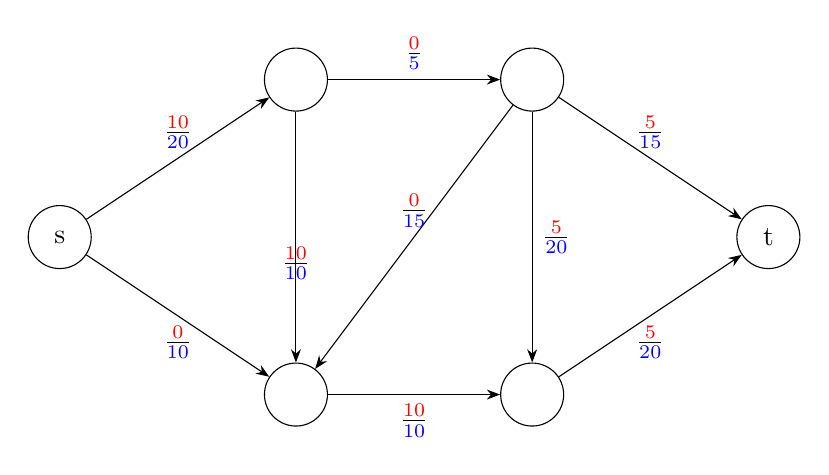
\begin{tikzpicture}[
          node distance=2.5cm,
          vertex/.style={circle, draw, minimum size=0.8cm},
          auto,
          >=Stealth
      ]

      % Nodes with increased horizontal spacing
      \node[vertex] (s) at (0,0) {s};
      \node[vertex] (a) at (3,2) {};
      \node[vertex] (b) at (6,2) {};
      \node[vertex] (c) at (3,-2) {};
      \node[vertex] (d) at (6,-2) {};
      \node[vertex] (t) at (9,0) {t};

      % Edges with colored fraction labels
      \draw[->] (s) -- node[above] {$\frac{\color{red}10}{\color{blue}20}$} (a);
      \draw[->] (s) -- node[below] {$\frac{\color{red}0}{\color{blue}10}$} (c);
      \draw[->] (a) -- node[above] {$\frac{\color{red}0}{\color{blue}5}$} (b);
      \draw[->] (a) -- node[below] {$\frac{\color{red}10}{\color{blue}10}$} (c);
      \draw[->] (b) -- node[above] {$\frac{\color{red}5}{\color{blue}15}$} (t);
      \draw[->] (b) -- node[right] {$\frac{\color{red}5}{\color{blue}20}$} (d);
      \draw[->] (c) -- node[below] {$\frac{\color{red}10}{\color{blue}10}$} (d);
      \draw[->] (d) -- node[below] {$\frac{\color{red}5}{\color{blue}20}$} (t);
      \draw[<-] (c) -- node[above] {$\frac{\color{red}0}{\color{blue}15}$} (b);

      \end{tikzpicture}
      \caption{The red values represent the flow. The blue values represent the capacity. The value of the above flow is 10.} 
      \label{fig:flow}
    \end{figure}

    Now let's revisit cuts. 

    \begin{definition}[Cuts]
      Given a flow network, a s-t \textbf{cut} is a partition of $V = S \sqcup T$ s.t. $s \in S, t \in T$. The \textbf{value}, or \textbf{capacity}, of a cut is defined as the capacity of its edges 
      \begin{equation}
        ||S, T|| = \sum_{u in S} \sum_{v \in T} C(u \rightarrow v)
      \end{equation}
    \end{definition}

    \begin{figure}[H]
      \centering 
      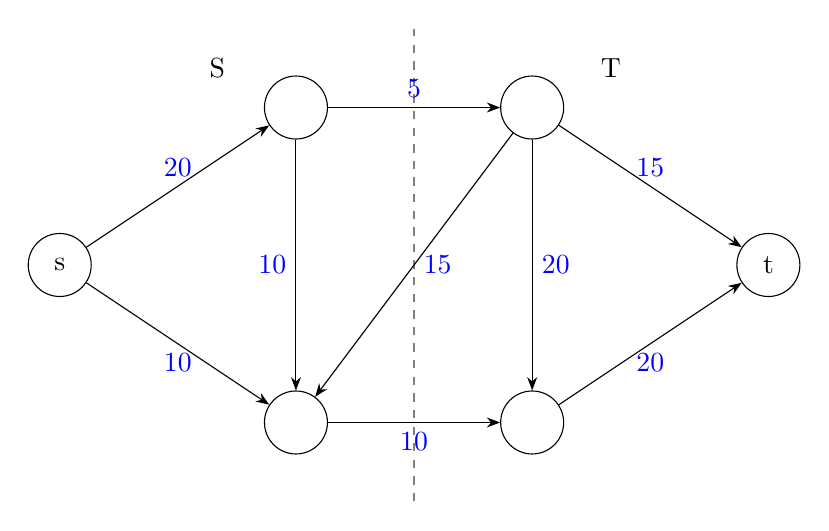
\begin{tikzpicture}[
          node distance=2.5cm,
          vertex/.style={circle, draw, minimum size=0.8cm},
          auto,
          >=Stealth
      ]

      % Nodes with increased horizontal spacing
      \node[vertex] (s) at (0,0) {s};
      \node[vertex] (a) at (3,2) {};
      \node[vertex] (b) at (6,2) {};
      \node[vertex] (c) at (3,-2) {};
      \node[vertex] (d) at (6,-2) {};
      \node[vertex] (t) at (9,0) {t};

      % Edges with upright colored fraction labels
      \draw[->] (s) -- node[above] {$\color{blue}20$} (a);
      \draw[->] (s) -- node[below] {$\color{blue}10$} (c);
      \draw[->] (a) -- node[above] {$\color{blue}5$} (b);
      \draw[->] (a) -- node[left] {$\color{blue}10$} (c);
      \draw[->] (b) -- node[above] {$\color{blue}15$} (t);
      \draw[->] (b) -- node[right] {$\color{blue}20$} (d);
      \draw[->] (c) -- node[below] {$\color{blue}10$} (d);
      \draw[->] (d) -- node[below] {$\color{blue}20$} (t);
      \draw[<-] (c) -- node[right] {$\color{blue}15$} (b);

      % Draw the cut (add this on background layer to appear behind nodes)
      \begin{scope}[on background layer]
          \draw[dashed, thick, gray] (4.5,-3) -- (4.5,3);
          
          % Add labels for the sets
          \node at (2,2.5) {S};
          \node at (7,2.5) {T};
      \end{scope}

      \end{tikzpicture}
      \caption{This cut has capacity 15. Note that the cut going from right to left is not included since this is a S-T cut. } 
      \label{fig:cut}
    \end{figure}

    We now introduce two related problems. 
    \begin{enumerate}
      \item Max Flow. How do we find the flow with the maximum value? This is analogous to maximizing the commodity transport from $s$ to $t$.  
      \item Min Cut. How do we find the cut with the minimum capacity? This is analogous to removing the smallest total edges that will disconnect $s$ to $t$. 
    \end{enumerate}

    \begin{theorem}[Max-Flow Min-Cut Theorem]
      For any valid $(s, t)$ flow $f$ on a flow network $G = (V, E)$ and any valid $(s, t)$-cut $S, T$, we have 
      \begin{equation}
        |f| \leq ||S, T||
      \end{equation} 
      It also turns out that equality is achieved, which immediately implies that the max-flow is the min-cut. 
    \end{theorem}
    \begin{proof}
      We can see that in order for a flow to have a value, given some cut the flow value cannot exceed the capacity through this cut from $S$ to $T$. Mathematically, we can see that the flow value is invariant due to conservation, and so  
      \begin{align}
        |f| & = \sum_{s \rightarrow v} f(s \rightarrow v) - \sum_{v \rightarrow s} f(v \rightarrow s) \\ 
            & = \sum_{u \in S} \sum_{v \in T} f(u \rightarrow v) - \sum_{v \in T} \sum_{u \in S} f(v \rightarrow u) \\ 
            & \leq \sum_{u \in S} \sum_{v \in T} c(u \rightarrow v) = ||S, T||
      \end{align}
    \end{proof} 

  \subsection{Maximum Flows}  

    Now to compute the maximum flow itself, we use a residual graph. For now, we will assume that a flow network $G$ does not have 2-cycles (cycles of length 2), and if we do find a graph with such a 2-cycle, we modify it by adding an intermediate node. 

    \begin{figure}[H]
      \centering 
      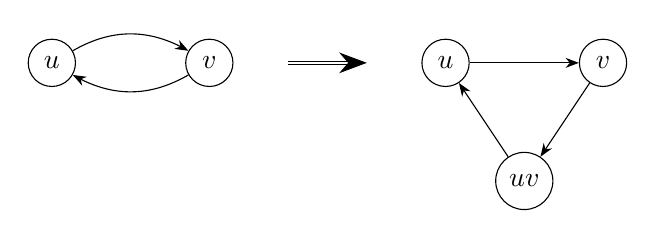
\begin{tikzpicture}[
          vertex/.style={circle, draw, minimum size=0.6cm},
          >=Stealth
      ]

      % First pattern
      \node[vertex] (u1) at (0,0) {$u$};
      \node[vertex] (v1) at (2,0) {$v$};

      \draw[->] (u1) to[bend left=30] (v1);
      \draw[->] (v1) to[bend left=30] (u1);

      % Arrow indicating transformation
      \draw[-{Stealth[length=10pt]}, double] (3,0) -- (4,0);

      % Second pattern
      \node[vertex] (u2) at (5,0) {$u$};
      \node[vertex] (v2) at (7,0) {$v$};
      \node[vertex] (uv2) at (6,-1.5) {$uv$};

      \draw[->] (u2) -- (v2);
      \draw[->] (v2) -- (uv2);
      \draw[->] (uv2) -- (u2);

      \end{tikzpicture}
      \caption{How we modify our 2-cycle.} 
      \label{fig:cycle_mod}
    \end{figure}

    \begin{definition}[Residual Network]
      Given a flow network $G$ and a flow $f$, the \textbf{residual graph} $G_f$ is a new flow network that has edges $u \rightarrow v$ and $v \rightarrow u$, where 
      \begin{equation}
        c_f (u \rightarrow v) = \begin{cases} c (u \rightarrow v) - f(u \rightarrow v) & \text{ if } u \rightarrow v \in E \\ 
          f(u \rightarrow v) & \text{ if } v \rightarrow u \in E
        \end{cases}
      \end{equation}
      Basically, if there is some flow in an edge, we replace that edge's capacity by the residual capacity, giving us our \textit{forward edge}, and then take this flow and add it to a new opposite pointing edge, called the \textit{backwards edge}. 
    \end{definition} 

    \begin{figure}[H]
      \centering 
      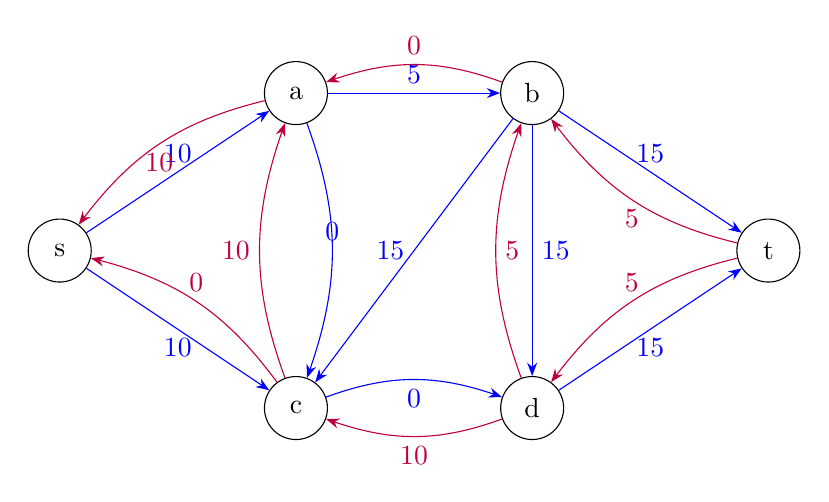
\begin{tikzpicture}[
          node distance=2.5cm,
          vertex/.style={circle, draw, minimum size=0.8cm},
          auto,
          >=Stealth,
          fwd/.style={blue},
          back/.style={purple}
      ]

      % Nodes with increased horizontal spacing
      \node[vertex] (s) at (0,0) {s};
      \node[vertex] (a) at (3,2) {a};
      \node[vertex] (b) at (6,2) {b};
      \node[vertex] (c) at (3,-2) {c};
      \node[vertex] (d) at (6,-2) {d};
      \node[vertex] (t) at (9,0) {t};

      % Forward edges in blue (including zero weights)
      \draw[->, fwd] (s) -- node[above] {10} (a);
      \draw[->, fwd] (s) -- node[below] {10} (c);
      \draw[->, fwd] (a) -- node[above] {5} (b);
      \draw[->, fwd] (b) -- node[above] {15} (t);
      \draw[->, fwd] (b) -- node[right] {15} (d);
      \draw[->, fwd] (b) -- node[left] {15} (c);
      \draw[->, fwd] (d) -- node[below] {15} (t);
      \draw[->, fwd] (a) to[bend left=20] node[above] {0} (c);
      \draw[->, fwd] (c) to[bend left=20] node[below] {0} (d);

      % Backward edges in purple (including zero weights)
      \draw[->, back] (a) to[bend right=20] node[below] {10} (s);
      \draw[->, back] (c) to[bend left=20] node[left] {10} (a);
      \draw[->, back] (d) to[bend left=20] node[below] {10} (c);
      \draw[->, back] (t) to[bend left=20] node[below] {5} (b);
      \draw[->, back] (t) to[bend right=20] node[above] {5} (d);
      \draw[->, back] (d) to[bend left=20] node[right] {5} (b);
      \draw[->, back] (c) to[bend right=20] node[above] {0} (s);
      \draw[->, back] (b) to[bend right=20] node[above] {0} (a);

      \end{tikzpicture}
      \caption{Residual network. } 
      \label{fig:residual_network}
    \end{figure}

    \begin{theorem}
      If we have a flow $f$, its value $|f|$ can be improved/augmented up to the bottleneck capacity on any residual path. That is, if we find any $s \rightarrow t$ path $\pi$ on $G_f$, with a positive bottleneck capacity (minimum capacity over its edges), we can improve the flow.\footnote{For example, the capacity of the path $S, C, A, B, T$ is $5$, since $A \rightarrow B$ has weight $5$.} Given this residual path $\pi$, it may have both forward or backwards edges. To augment the original path on $G$ by value $b$, we look at each edge $(u \rightarrow v) \in E$ and 
      \begin{enumerate}
        \item If it corresponds to a forward edge (i.e. if $(u \rightarrow v)$ is in the residual path $\pi$), we add $b$. This corresponds to how much more flow you can put into this edge. 
        \item If it corresponds to a backward edge (i.e. if $(v \rightarrow u)$ is in the residual path $\pi$), we subtract $b$. The corresponds to how much flow could you reroute in the backwards direction and have it reach $t$ through another path.   
        \item If it is not in $\pi$, then we don't change it. 
      \end{enumerate}
      In summary, the new flow $f^\prime$ is defined 
      \begin{equation}
        f^\prime (u \rightarrow v) = \begin{cases} 
          f(u \rightarrow v) + b & \text{ if } (u \rightarrow v) \in \pi \\ 
          f(u \rightarrow v) - b & \text{ if } (v \rightarrow u) \in \pi \\  
          f(u \rightarrow v) & \text{ else }
        \end{cases}
      \end{equation}
    \end{theorem} 
    \begin{proof}
      We first show that $f^\prime$ is a valid flow. For feasibility, 
      \begin{enumerate}
        \item \textit{Forward}. If $(u \rightarrow  v) \in \pi$, then 
          \begin{equation}
            f^\prime (u \rightarrow v) = f(u \rightarrow v) + b \leq f(u \rightarrow v) + c_f (u \rightarrow v) = c(u \rightarrow v)
          \end{equation} 
        \item \textit{Backward}. If $(v \rightarrow u) \in \pi$, then 
          \begin{equation}
          f^\prime (u \rightarrow v) = f(u \rightarrow v) - b \geq f(u \rightarrow v) - c_f (v \rightarrow u) = 0 
          \end{equation}
      \end{enumerate}

      For conservation, there are 4 cases. 
      \begin{enumerate}
        \item Forward into node, forward out of node. $\Delta_{in} = +b, \Delta_{out} = +b$. Therefore the flows cancel out. 
        \item Forward into node, backward out of node. $\Delta_{in} = +b - b = 0$. 
        \item Backward into node, forward out of node. $\Delta_{out} = +b - b = 0$. 
        \item Backward into node, backward out of node. $\Delta_{in} = -b, \Delta_{out} = - b$. 
      \end{enumerate}
    \end{proof} 

    At this point, we're pretty much ready to give our algorithm on max-flow. 

    \begin{algo}[Ford-Fulkerson]
      We've reduced this problem to a problem of finding a positive path $\pi$ in the residual graph, which we have a lot of algorithms built for. We find such a path and augment the flow until we cannot find such a path. If we cannot find a path, then we can use BFS to look at all vertices $S \subset V$ reachable from $s$ in $G_f$, and then let $T = V \setminus S$. These two disjoint sets will give the min cut. 
      
      \begin{algorithm}[H]
        \label{alg:maxflow}
        \begin{algorithmic}
          \Require{Flow network $G(V, E)$, source/sink $s, t \in V$. Capacity $c$. }
          \State 
          \Function{MaxFlow}{G}
          \State Start with the trivial flow $f$, maybe stored as array $[0, \ldots, 0]$ of length $E$. 
            \State Construct residual graph $G_f$ for this trivial flow. 
            \While{$G_f$ has an augmenting path in $G_f$} \Comment{Maybe use BFS to find this.}
              \State Pick $\pi$ as any augmenting path 
              \State augment $f$ by bottleneck capacity 
              \State update $G_f$. 
            \EndWhile
            \State \Return{f}  
            \State Use BFS to find all nodes in $G_f$ reachable from $s$. Call this $S$.  
            \State Let $T = V \setminus S$.  
            \State $S, T$ is our min cut, and $f$ is your max flow. 
          \EndFunction
        \end{algorithmic}
      \end{algorithm}
      The inner loop is just BFS, which is $O(N + M)$, but how many iterations do we do? Well for integer capacities, we can bound it by the actual value of the max flow $|f^\ast|$ since we must improve by at least $+1$ every loop.\footnote{This is not a trivial result that if all capacities are integers, then there is an integer max-flow, despite the actual flow being dispersed as fractions across edges.} Unfortunately, $O((N+M) |f^\ast|)$ is the best we can do in generality, which is pseudopolynomial. 
    \end{algo}

    There are indeed polynomial time algorithms, e.g. Orlin's algorithm with runtime $O(NM)$, which is guaranteed to be polynomial but in practice may be slower. 

    \begin{example}[Max Flow and Residual Graph]
      Here is the max flow. 
      \begin{figure}[H]
        \centering
        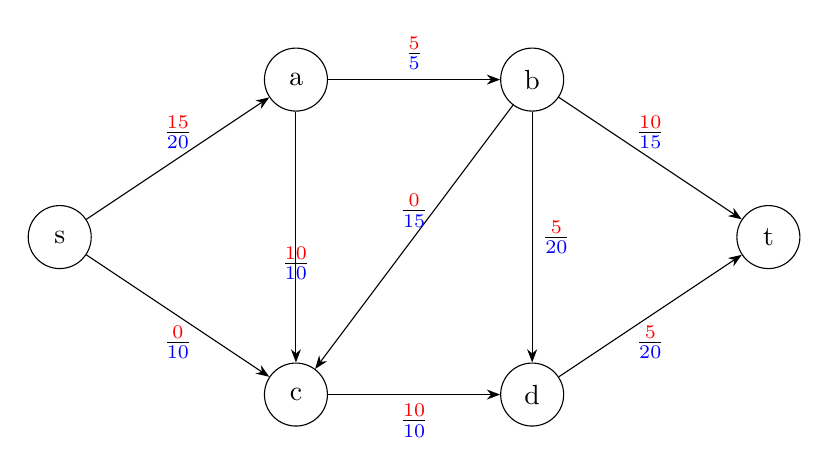
\begin{tikzpicture}[
            node distance=2.5cm,
            vertex/.style={circle, draw, minimum size=0.8cm},
            auto,
            >=Stealth
        ]

        % Nodes with increased horizontal spacing
        \node[vertex] (s) at (0,0) {s};
        \node[vertex] (a) at (3,2) {a};
        \node[vertex] (b) at (6,2) {b};
        \node[vertex] (c) at (3,-2) {c};
        \node[vertex] (d) at (6,-2) {d};
        \node[vertex] (t) at (9,0) {t};

        % Edges with colored fraction labels
        \draw[->] (s) -- node[above] {$\frac{\color{red}15}{\color{blue}20}$} (a);
        \draw[->] (s) -- node[below] {$\frac{\color{red}0}{\color{blue}10}$} (c);
        \draw[->] (a) -- node[above] {$\frac{\color{red}5}{\color{blue}5}$} (b);
        \draw[->] (a) -- node[below] {$\frac{\color{red}10}{\color{blue}10}$} (c);
        \draw[->] (b) -- node[above] {$\frac{\color{red}10}{\color{blue}15}$} (t);
        \draw[->] (b) -- node[right] {$\frac{\color{red}5}{\color{blue}20}$} (d);
        \draw[->] (c) -- node[below] {$\frac{\color{red}10}{\color{blue}10}$} (d);
        \draw[->] (d) -- node[below] {$\frac{\color{red}5}{\color{blue}20}$} (t);
        \draw[<-] (c) -- node[above] {$\frac{\color{red}0}{\color{blue}15}$} (b);

        \end{tikzpicture}
        \caption{The max flow of the above graph.}
        \label{fig:ex_flow}
      \end{figure}
      Here is the residual graph, which shows indeed that this the max flow. The min cut is therefore $S = \{s, a, c\}$ and $T = \{t, b, d\}$. 
      \begin{figure}[H]
        \centering
        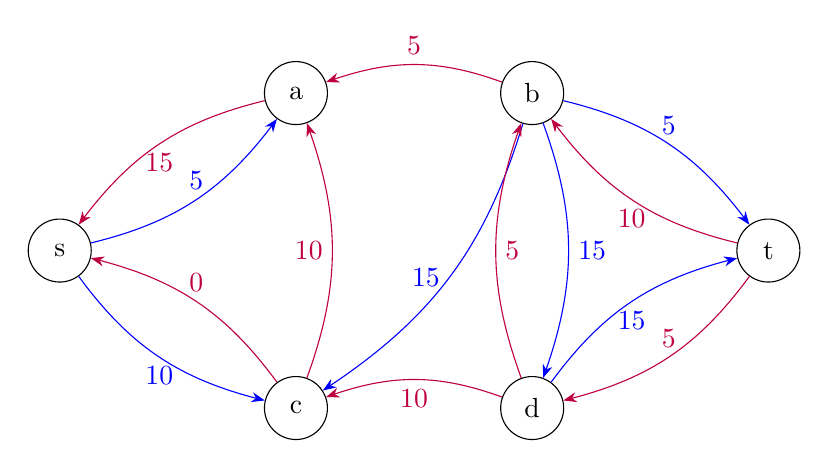
\begin{tikzpicture}[
            node distance=2.5cm,
            vertex/.style={circle, draw, minimum size=0.8cm},
            auto,
            >=Stealth,
            fwd/.style={blue},
            back/.style={purple}
        ]

        % Nodes with increased horizontal spacing
        \node[vertex] (s) at (0,0) {s};
        \node[vertex] (a) at (3,2) {a};
        \node[vertex] (b) at (6,2) {b};
        \node[vertex] (c) at (3,-2) {c};
        \node[vertex] (d) at (6,-2) {d};
        \node[vertex] (t) at (9,0) {t};

        % Forward residual edges (blue) capacity-flow
        \draw[->, fwd] (s) to[bend right=20] node[above] {5} (a);  % 20-15=5
        \draw[->, fwd] (s) to[bend right=20] node[below] {10} (c); % 10-0=10
        \draw[->, fwd] (b) to[bend left=20] node[above] {5} (t);  % 15-10=5
        \draw[->, fwd] (b) to[bend left=20] node[right] {15} (d); % 20-5=15
        \draw[->, fwd] (b) to[bend left=20] node[left] {15} (c);  % 15-0=15
        \draw[->, fwd] (d) to[bend left=20] node[below] {15} (t); % 20-5=15

        % Backward residual edges (purple) flow
        \draw[->, back] (a) to[bend right=20] node[below] {15} (s); % flow=15
        \draw[->, back] (c) to[bend right=20] node[left] {10} (a);  % flow=10
        \draw[->, back] (d) to[bend right=20] node[below] {10} (c); % flow=10
        \draw[->, back] (t) to[bend left=20] node[below] {10} (b); % flow=10
        \draw[->, back] (t) to[bend left=20] node[above] {5} (d);   % flow=5
        \draw[->, back] (d) to[bend left=20] node[right] {5} (b);  % flow=5
        \draw[->, back] (b) to[bend right=20] node[above] {5} (a);  % flow=5
        \draw[->, back] (c) to[bend right=20] node[above] {0} (s);   % flow=0

        \end{tikzpicture}
        \caption{You can see that there are no paths from $s$ to $t$ anymore. The edges $a \rightarrow b$ and $c \rightarrow d$ in the original graph are saturated and so have weight $0$ in the residual graph. }
        \label{fig:ex_residual}
      \end{figure}
    \end{example} 

    \begin{example}[Edge Disjoint Paths]
      Given a directed graph $G(V, E)$ with start and end nodes $s, t \in V$, we want to find the maximum number of paths from $s \rightarrow t$ s.t. they do not share any edge, i.e. are \textit{edge-disjoint}. 
      \begin{figure}[H]
        \centering 
        \caption{This graph has two edge-disjoint paths: the top and bottom paths. } 
        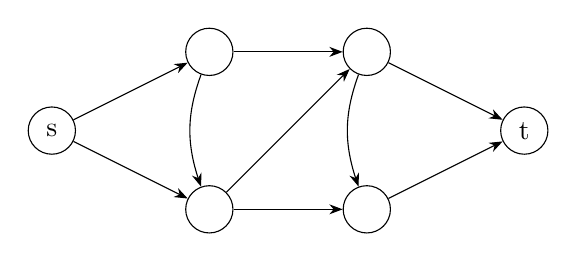
\begin{tikzpicture}[
            vertex/.style={circle, draw, minimum size=0.6cm},
            >=Stealth
        ]

        % Nodes - arranging them in the shape shown
        \node[vertex] (s) at (0,0) {s};
        \node[vertex] (a) at (2,1) {};
        \node[vertex] (b) at (4,1) {};
        \node[vertex] (t) at (6,0) {t};
        \node[vertex] (c) at (2,-1) {};
        \node[vertex] (d) at (4,-1) {};

        % Upper and lower path edges
        \draw[->] (s) -- (a);
        \draw[->] (a) -- (b);
        \draw[->] (b) -- (t);
        \draw[->] (s) -- (c);
        \draw[->] (c) -- (d);
        \draw[->] (d) -- (t);

        % Cross edges between paths
        \draw[->] (a) to[bend right=20] (c);
        \draw[->] (c) -- (b);
        \draw[->] (b) to[bend right=20] (d);

        \end{tikzpicture}
        \label{fig:edge_disjoint}
      \end{figure}
      
      The idea is to reduce the maximum flow by first assigning capacity 1 to every edge. Then we compute the maximum flow $f^\ast$, and then return $|f^\ast|$. It turns out that even if we chose a path $\pi$ that went through the center node, the augmentation would push us to redirect the flows to the top and bottom outer edges. Since $|f^\ast| \leq n-1 < m$ in this example (since it can be at most the maximum indegree or outdegree of $s, t$), we should probably use Ford-Fulkerson rather than Orlin's algorithm. 
    \end{example}

    This leads to the lemma. 

    \begin{theorem}[Edge-Disjoint Paths]
      Given directed graph $G$ and its corresponding flow network $G^\prime$ of capacity $1$, the following are true: 
      \begin{enumerate}
        \item If there exists $k$ edge-disjoint paths in $G$, then there exists a flow with value $\geq k$ in $G^\prime$. 
        \item If there exists a flow of value $k$ in $G^\prime$, then there exists $k$ edge-disjoint paths in $G$. 
      \end{enumerate}
    \end{theorem}
    \begin{proof}
      The first is trivially feasible and conservation is satisfied since for any node $u \in V \setminus \{s, t\}$, every path in $P$ (the collection of $k$ paths) that enters $u$ must exit $u$, so the total flow in equals the total flow out $\implies$ $f$ is a valid $(s, t)$-flow. Therefore, we have $k$ paths leaving $s$, so $|f| = k$. 

      For the other direction, let $f$ be the flow with value $k$, and let $P = \{\}$. Let $H$ be the subgraph of $G^\prime$ of edges with positive flow, and for every loop, we use BFS from $s$ to $t$ to get a path $\pi$. We then add $\pi$ to $P$ and remove $\pi$ from $H$, repeat this $k$ times until we get $k$ paths in $P$.  
    \end{proof} 

    The way that we have constructed a collection of paths from a flow function is very useful, and is called \textit{flow decomposition}. We can go back and forth between a flow and a collection of paths by doing what we have just done in the previous proof. 

    \begin{definition}[Flow Decomposition]
      Given a general flow $f$ on flow network $G$, we initialize our set of paths $P = \{\}$ and loop the following: 
      \begin{enumerate}
        \item Use BFS from $s$ to $t$ to get a path $\pi$. 
        \item Add $\pi$ to $P$ and rather than strictly removing the path from $H$, we need to be mindful of how much flow is left on it after removing only the bottleneck flow on the path. 
      \end{enumerate}
      This can be done in $O(NM)$ time, which loosely is because we are running BFS $O(M)$ times. 
    \end{definition}

    \begin{example}[Undirected Edge-Disjoint Paths]
      What if $G$ is undirected? In this case, we want to construct a flow network and then convert its 2 cycles into a 3 cycles by adding artificial points, taking linear time. 
    \end{example}

    \begin{example}[Undirected Edge-Disjoint Paths]
      Another problem is about vertex-disjoint paths, which is a stronger restriction than edge-disjoint ones. Each node does not have a concept of a capacity, so the general idea is for each vertex $v$, replace it with an ``in-out gadget'' with an edge of weight 1. The rest of the details follow similarly from edge-disjoint paths. 
      
      \begin{figure}[H]
        \centering 
        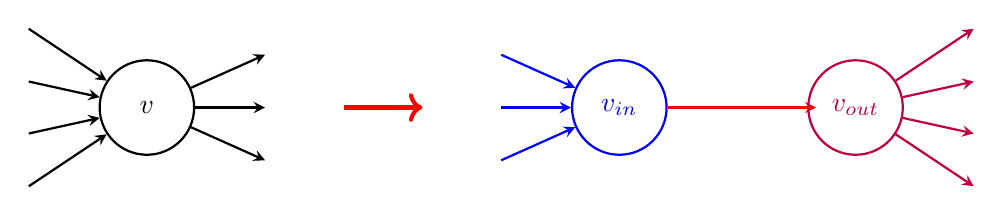
\begin{tikzpicture}

        % Define styles
        \tikzset{
            voltage node/.style={
                draw,
                circle,
                minimum size=1.2cm,
                thick
            },
            arrow style/.style={
                ->,
                >=stealth,
                thick
            }
        }

        % Left figure
        % Node v with 4 in-edges and 3 out-edges
        \node[voltage node] (v1) at (0,0) {$v$};

        % In-edges
        \draw[arrow style] (-1.5, 1) -- (v1);
        \draw[arrow style] (-1.5, 0.33) -- (v1);
        \draw[arrow style] (-1.5, -0.33) -- (v1);
        \draw[arrow style] (-1.5, -1) -- (v1);

        % Out-edges
        \draw[arrow style] (v1) -- (1.5, 0.67);
        \draw[arrow style] (v1) -- (1.5, 0);
        \draw[arrow style] (v1) -- (1.5, -0.67);

        % Arrow between figures
        \draw[->, line width=1.5pt, red] (2.5,0) -- (3.5,0);

        % Right figure
        % Node v_in with 3 in-edges
        \node[voltage node, blue] (v2) at (6,0) {$v_{in}$};
        \draw[arrow style, blue] (4.5, 0.67) -- (v2);
        \draw[arrow style, blue] (4.5, 0) -- (v2);
        \draw[arrow style, blue] (4.5, -0.67) -- (v2);

        % Connection between v_in and v_out
        \draw[arrow style, red] (v2) -- (8.5,0);

        % Node v_out with 4 out-edges
        \node[voltage node, purple] (v3) at (9,0) {$v_{out}$};
        \draw[arrow style, purple] (v3) -- (10.5, 1);
        \draw[arrow style, purple] (v3) -- (10.5, 0.33);
        \draw[arrow style, purple] (v3) -- (10.5, -0.33);
        \draw[arrow style, purple] (v3) -- (10.5, -1);

        \end{tikzpicture}
        \caption{} 
        \label{fig:undirected_ex}
      \end{figure}
    \end{example}

    \begin{example}[Maximum Bipartite Matching]
      Another application is in \textbf{bipartite matching}, which for an undirected bipartite graph $G(V, E)$ with $V = A \sqcup B$, is a subset of the edges $M \subset E$ s.t. no 2 edges in $M$ share an endpoint. The goal is to find the maximum bipartite matching, i.e. the matching with the greatest total weight. 

      \begin{figure}[H]
        \centering 
        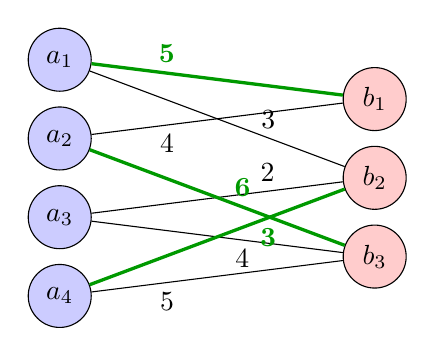
\begin{tikzpicture}[
            blue node/.style={draw, circle, fill=blue!20, minimum size=0.8cm},
            red node/.style={draw, circle, fill=red!20, minimum size=0.8cm},
            normal edge/.style={thin, black},
            matching edge/.style={very thick, green!60!black},
            normal weight/.style={black},
            matching weight/.style={green!60!black, font=\bfseries}
        ]

        % Left (blue) nodes
        \node[blue node] (a1) at (0,3) {$a_1$};
        \node[blue node] (a2) at (0,2) {$a_2$};
        \node[blue node] (a3) at (0,1) {$a_3$};
        \node[blue node] (a4) at (0,0) {$a_4$};

        % Right (red) nodes
        \node[red node] (b1) at (4,2.5) {$b_1$};
        \node[red node] (b2) at (4,1.5) {$b_2$};
        \node[red node] (b3) at (4,0.5) {$b_3$};

        % Regular edges with weights
        \draw[normal edge] (a1) -- node[above, pos=0.7] {3} (b2);
        \draw[normal edge] (a2) -- node[below, pos=0.3] {4} (b1);
        \draw[normal edge] (a3) -- node[above, pos=0.7] {2} (b2);
        \draw[normal edge] (a3) -- node[below, pos=0.6] {4} (b3);
        \draw[normal edge] (a4) -- node[below, pos=0.3] {5} (b3);

        % Maximum matching edges (highlighted in green)
        \draw[matching edge] (a1) -- node[above, pos=0.3, matching weight] {5} (b1);
        \draw[matching edge] (a2) -- node[above, pos=0.6, matching weight] {6} (b3);
        \draw[matching edge] (a4) -- node[below, pos=0.7, matching weight] {3} (b2);

        \end{tikzpicture}
        \caption{A bipartite matching} 
        \label{fig:bipartite_matching}
      \end{figure}

      The general idea is to take an undirected graph, convert it to a flow network, compute the max flow, i.e. min cut, and then translate it back into the undirected graph solution.  
      \begin{enumerate}
        \item Construct the flow network $G^\prime = (V^\prime, E^\prime)$, where $V^\prime = V \cup \{s, t\}$, with additional edges going from $s$ to $A$ and $B$ to $t$ all with weights $1$. Replace the middle edges with directed edges towards the flow with the same weight (though it can be any weight at least 1). 

        \begin{figure}[H]
          \centering 
          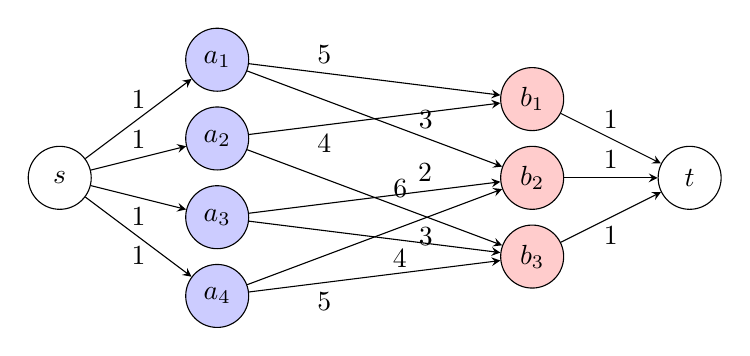
\begin{tikzpicture}[
              blue node/.style={draw, circle, fill=blue!20, minimum size=0.8cm},
              red node/.style={draw, circle, fill=red!20, minimum size=0.8cm},
              special node/.style={draw, circle, minimum size=0.8cm},
              edge/.style={->, >=stealth}
          ]

          % Source and sink nodes
          \node[special node] (s) at (-2,1.5) {$s$};
          \node[special node] (t) at (6,1.5) {$t$};

          % Left (blue) nodes
          \node[blue node] (a1) at (0,3) {$a_1$};
          \node[blue node] (a2) at (0,2) {$a_2$};
          \node[blue node] (a3) at (0,1) {$a_3$};
          \node[blue node] (a4) at (0,0) {$a_4$};

          % Right (red) nodes
          \node[red node] (b1) at (4,2.5) {$b_1$};
          \node[red node] (b2) at (4,1.5) {$b_2$};
          \node[red node] (b3) at (4,0.5) {$b_3$};

          % Edges from source to A nodes with weight 1
          \draw[edge] (s) -- node[above] {1} (a1);
          \draw[edge] (s) -- node[above] {1} (a2);
          \draw[edge] (s) -- node[below] {1} (a3);
          \draw[edge] (s) -- node[below] {1} (a4);

          % Edges from B nodes to sink with weight 1
          \draw[edge] (b1) -- node[above] {1} (t);
          \draw[edge] (b2) -- node[above] {1} (t);
          \draw[edge] (b3) -- node[below] {1} (t);

          % Middle edges (directed A to B) with original weights
          \draw[edge] (a1) -- node[above, pos=0.3] {5} (b1);
          \draw[edge] (a1) -- node[above, pos=0.7] {3} (b2);
          \draw[edge] (a2) -- node[below, pos=0.3] {4} (b1);
          \draw[edge] (a2) -- node[above, pos=0.6] {6} (b3);
          \draw[edge] (a3) -- node[above, pos=0.7] {2} (b2);
          \draw[edge] (a3) -- node[below, pos=0.6] {4} (b3);
          \draw[edge] (a4) -- node[below, pos=0.7] {3} (b2);
          \draw[edge] (a4) -- node[below, pos=0.3] {5} (b3);

          \end{tikzpicture}

          \label{fig:g_prime}
        \end{figure}

        \item Compute max flow $f$ in $G^\prime$. 
        \item Return $M = \{ (u \rightarrow v) \in E \mid f(u \rightarrow v) = 1 \}$. This can be done using the flow decomposition or just by looking at the edges in our flow with value $1$ and mapping it to the corresponding undirected bipartite graph. 
      \end{enumerate}
      To see correctness, we claim that there exists a matching $M$ in $G$ of size $k$ iff there exists a flow $f$ in $G^\prime$ with $|f|= k$, and therefore the max matching corresponds to the max flow. Constructing the flow network is $O(N + M)$ since $N^\prime = N + 2$ and $M^\prime = M + N$. Computing the max-flow is $O(N^\prime M^\prime)$ or $O(M^\prime |f|)$ depending on if we use Orlin's or Ford-Fulkerson, but either one is $O(NM)$. Then mapping it back to $M$ might take $O(M)$, so the total time is $O(NM)$. 
    \end{example}

\section{Efficiency} 

  \subsection{NP-Completeness and Reductions} 

    We have talked about optimization problems that choose the best solution from a class of solutions. Now we will talk about \textit{decision problems}, which seek to answer whether a certain problem contains a solution or not. Here are two examples. It turns out we can convert one into the other easily by rephrasing the problem. 

    \begin{definition}[CircuitSAT]
      Consider a black box circuit $f$, with input $\mathbf{x} \in \{0, 1\}^n$. We want to answer the question of whether there exists some $\mathbf{x}$ s.t. $f(\mathbf{x}) = 1$, i.e. whether the circuit is \textbf{satisfiable}? 

      \begin{figure}[H]
        \centering 
        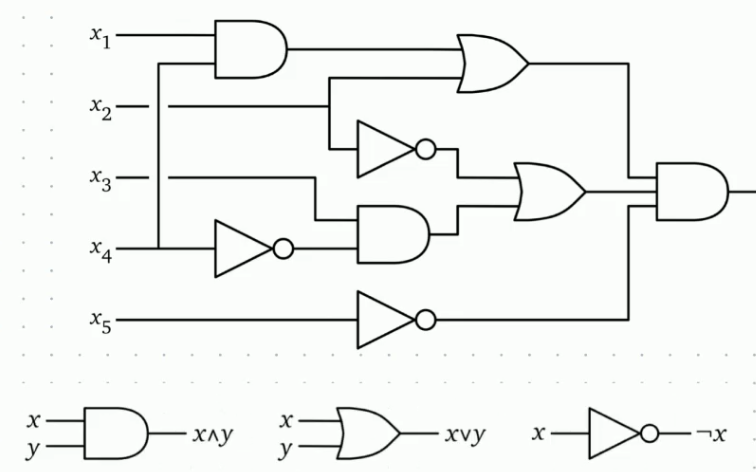
\includegraphics[scale=0.4]{img/circuit.png}
        \caption{Some random circuit where $n = 5$.} 
        \label{fig:random_circuit}
      \end{figure}
      The obvious way is to brute force is an check all $2^n$ combinations, and this is the only way since this is black-box. However, even if we knew the circuit itself, the amount of computations that we need to solve this is conjectured to be still $O(2^n)$, though we may be able to cleverly shave off some calculations here and there.\footnote{It is not proven that there exists no exponential algorithm.}
    \end{definition}

    \begin{definition}[3SAT]
      Given a boolean formula $\phi$ where each \textbf{clause} contains exactly 3 literals, determine if there exists a satisfying assignment to the variables that makes $\phi$ true. Formally:
      \begin{align*}
        \phi &= C_1 \land C_2 \land \cdots \land C_m \\
        C_i &= (l_{i1} \lor l_{i2} \lor l_{i3}) \\
        l_{ij} &\in \{x_k, \neg x_k\} \text{ for some } k \in \{1,\ldots,n\}
      \end{align*}
      where $x_k$ are boolean variables and $\neg x_k$ their negations. For example:
      \begin{align*}
        \phi = (x_1 \lor \neg x_2 \lor x_3) \land (\neg x_1 \lor x_2 \lor x_4) \land (x_2 \lor \neg x_3 \lor \neg x_4)
      \end{align*}
      Like CircuitSAT, this problem is also believed to require $O(2^n)$ time, and in fact these problems are polynomially reducible to each other (CircuitSAT $\leq_p$ 3SAT and 3SAT $\leq_p$ CircuitSAT). The key difference is that 3SAT has a very specific structure that makes it easier to analyze and reduce other problems to, making it a canonical NP-complete problem.\footnote{The restriction to exactly 3 literals per clause is not arbitrary - 2SAT is solvable in polynomial time, while 3SAT is NP-complete.}
    \end{definition}

    In fact, there is a polynomial time algorithm to translate between 3SAT and CircuitSAT, so the two are theoretically equivalent. 

    \begin{definition}[Classes of Problems]
      Given the set of all decision problems. 
      \begin{enumerate}
        \item $P$ (Polynomial Time) is the set of all decision problems with polynomial-time algorithms. 
        \item $NP$ (Nondeterministic Polynomial Time) is the set of all decision problems for which if it returns $1$ (i.e. a solution exists), this can be \textit{verified} in polynomial time. 
      \end{enumerate}
      Clearly, $P$ is more restrictive since if we can solve a problem in polynomial time, it can be verified in polynomial time (again if a solution exists). If a solution doesn't exist, we would have to show that no solutions exist by testing all cases. So 
      \begin{equation}
        P \subset NP
      \end{equation}
      There can be other problems which are at least as hard as NP, called \textbf{NP-hard}. The intersection of NP-hard and NP is \textbf{NP-complete}, which can be thought of as the hardest problems existing in NP.\footnote{We will deal with P vs NP problems only in the context of decision problems, but we can classify optimization problems as NP-hard. }

      \begin{figure}[H]
        \centering 
        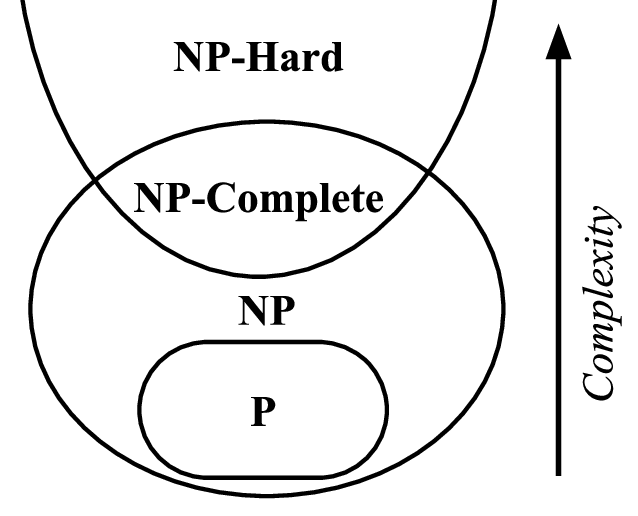
\includegraphics[scale=0.3]{img/class.png}
        \caption{Diagram of the 4 classes. The complexity rises as we go up. } 
        \label{fig:class}
      \end{figure}
    \end{definition}

    The other way around $NP \subset P$ is an unsolved millenium conjecture. It attempts to answer what the runtime difference or difficulty is between solving and verifying a problem? The conjecture states that solving is exponentially harder that verifying. 

    \begin{theorem}[Formal Definition of NP-hard Problems]
      A problem $\pi$ is NP-hard iff the existence of a polynomial time algorithm for $\pi$ implies $P = NP$. 
    \end{theorem}

    \begin{theorem}
      For CircuitSAT, 
      \begin{equation}
        \texttt{CircuitSAT} \not\in P, \texttt{CircuitSAT} \in NP
      \end{equation}
      That is, it cannot be solved in polynomial time, but given a solution circuit and a satisfying assignment, the assignment can be verified in $O(N+M)$ time. 
      For 3SAT, 
      \begin{equation}
        \texttt{3SAT} \not\in P, \texttt{3SAT} \in NP
      \end{equation}
      That is, it cannot be solved in polynomial time, but given a solution formula and a satisfying assignment, the assignment can be verified in $O(N+M)$ time. 
    \end{theorem}

    \begin{theorem}[Cook-Levin]
      3SAT is NP-complete. 
    \end{theorem}

    \begin{theorem}[Longest Path]
      Finding the longest path in a graph is NP-complete. 
    \end{theorem}

    To show whether a problem is NP, we should show that it is verifiable in polynomial time, which we have done so far. 

    \begin{definition}[Reduction]
      For NP-hard, we use a technique called \textit{reduction}. In other words, to prove a problem $\pi$ is NP-hard, reduce a known NP-hard problem $\beta$ to $\pi$ in polynomial time (not the other way around!). If this reduction is possible, then $\pi$ must be at least as hard as $\beta$: $\beta \leq_p \pi$, i.e. there exists an injective (but not necessarily surjective) mapping from the set of solutions of $\beta$ to the set of solutions of $\pi$. Formally, 
      \begin{enumerate}
        \item Assume there exists a polynomial time algorithm that solves $\pi$. 
        \item Since we have reduced $\pi$ to $\beta$, this indicates that we can use this polytime algorithm to solve $\beta$, which we already knew was NP-hard. 
        \item This creates a contradiction, and therefore $\pi$ must be NP-hard. 
      \end{enumerate}
    \end{definition}

    For example, to prove that CircuitSAT is NP-hard, we should reduce 3-SAT to CircuitSAT in polynomial time and then we are done.  

    \begin{example}[MIS]
      Given an undirected graph $G(V, E)$, an \textbf{independent set} is a subset $S \subseteq V$ such that no two vertices in $S$ are connected by an edge in $E$. The Maximum Independent Set problem asks us to find an independent set of maximum cardinality. 
    \end{example}

    \begin{theorem}[Maximum Independent Set (MIS)]
      MIS is NP-hard.
    \end{theorem}
    \begin{proof}
      We prove NP-hardness by reducing from 3SAT, which is more structured than CircuitSAT. Given a 3SAT instance $\phi$, we construct a graph $G$ such that $\phi$ is satisfiable if and only if $G$ has an independent set of size $m$, where $m$ is the number of clauses in $\phi$. The reduction works as follows: For a 3SAT formula $\phi = C_1 \land C_2 \land \cdots \land C_m$ where each clause $C_i = (l_{i1} \lor l_{i2} \lor l_{i3})$, construct graph $G(V,E)$:

      \begin{enumerate}
        \item For each clause $C_i$, create a \textbf{clause gadget}: a triangle with vertices labeled $l_{i1}$, $l_{i2}$, and $l_{i3}$ with undirected edges between them. 
        \item Add \textbf{consistency edges}: for any two literals $l_{ij}$ and $l_{k\ell}$ from different triangles, add an edge if they are complementary (i.e., one is $x$ and the other is $\neg x$)
      \end{enumerate}

      This reduction has the following properties:
      \begin{itemize}
        \item Each triangle forces us to choose at most one literal from each clause
        \item Consistency edges ensure we can't choose contradictory literals
        \item Choosing $m$ vertices (one per triangle) corresponds to making each clause true
      \end{itemize}

      It turns out that $\phi$ is satisfiable iff the size of the IS in $G$ is exactly the number of clauses in $phi$. 
      \begin{itemize}
        \item ($\Rightarrow$) If $\phi$ is satisfiable, choose one true literal from each clause to form an independent set of size $m$
        \item ($\Leftarrow$) If $G$ has an independent set of size $m$, it must contain exactly one vertex per triangle (by pigeonhole principle), giving us a valid satisfying assignment
      \end{itemize}

      Therefore, now that we have established the reduction, since 3SAT is NP-complete and we have a polynomial-time reduction to MIS, MIS is NP-hard.
    \end{proof}

    \begin{example}[3SAT Reduction of MIS]
      Consider the 3SAT formula 
      \begin{equation}
        \phi = (a \lor b \lor c) \land (b \lor \neg c \lor \neg d) \land (\neg a \lor c \lor d) \land (a \lor \neg b \lor \neg d)
      \end{equation}
      Following our reduction, we construct graph $G$ as follows:

      \begin{figure}[H]
        \centering 
        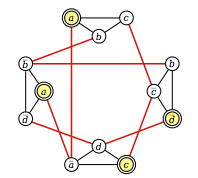
\includegraphics[scale=0.8]{img/mis_graph.png}
        \caption{Reduction graph from 3SAT to MIS. } 
        \label{fig:mis_graph}
      \end{figure}

      The graph contains:
      \begin{enumerate}
        \item Four triangles, one for each clause of $\phi$
        \item Red edges connecting complementary literals (e.g., $b$ with $\bar{b}$)
        \item A maximum independent set highlighted in yellow ($\{a, d\}$) of size 4
      \end{enumerate} 

      This independent set corresponds to the satisfying assignment $(a, b, c, d) = (1, \ast, 1, 0)$. 
      \begin{itemize}
        \item $(a \lor b \lor c)$ is satisfied by $a = 1$
        \item $(b \lor \neg c \lor \neg d)$ is satisfied by $d = 0$. 
        \item $(\neg a \lor c \lor d)$ is satisfied by $c = 1$. 
        \item $(a \lor \neg b \lor \neg d)$ is satisfied by $a = 1$. 
      \end{itemize}

      To demonstrate the proof, we assume that this MIS can be solved in polynomial time, so $MIS \in P$. But since $3SAT \leq_p MIS$, this means that $3SAT \in P$, which is a contradiction since $3SAT \in NP-hard$. 
    \end{example} 

    \begin{example}[Min Vertex Cover]
      Given an undirected graph $G(V, E)$, a \textbf{vertex cover} is a subset $S \subset V$ where for all $(u, v) \in E$, either $u \in S$ or $v \in S$ (or both). We would like to figure out the vertex cover of minimum cardinality, i.e. the min vertex cover. 
    \end{example}

    \begin{theorem}[MVC]
      MVC is NP-hard. 
    \end{theorem}
    \begin{proof}
      We will reduce this from MIP. Recall that an independent set is a subset $S \subset V$ s.t. for all $(u, v) \in E$, $u \in S$ or $v \in S$. By definition, we can see that $u \in S \iff u \not\in V \setminus S$, and so IS and VCs are related in the following way: 
      \begin{equation}
        S \subset V \text{ is a VC} \iff V \setminus S \text{ is an IS of size } n-k
      \end{equation}

      We assume that a polytime algorithm exists for MVC, so on input $G(V, E0)$, we calculate the MVC, call it $M$, and then we return the corresponding maxiumum independent set $S = V \setminus M$. But this would imply that there exists such a polytime algorithm, implying that $P = NP$, and therefore MVC must be NP-hard by definition. 
    \end{proof}

    \begin{example}[Max Clique]
      Given an undirected graph $G(V, E)$, a \textbf{clique} a subset of vertices $S \subset V$ s.t. there is an edge between each pair in $S$, i.e. a \textit{complete subgraph}. We would like to find the largest clique. 
    \end{example} 

    \begin{theorem}[MC]
      Finding the max clique is NP-hard. 
    \end{theorem}
    \begin{proof}
      Let's define the \textbf{edge-complement} of a graph $G$ as $\bar{G} = (V, \bar{E})$ where $\bar{E}$ is the set of edges not in $G$. Note that if $S \subset V$ is an independent set of $G$, then for all $u, v \in S$, $(u, v) \not\in E$, which is equivalent saying that $(u, v) \in \bar{E}$, which means that $S \subset V$ is a clique of $\bar{G}$. 

      Therefore, we can reduce this from MIS by taking input $G$, getting $\bar{G}$ in $O(N + M)$ time, and returning the size of the max clique of $\bar{G}$ in our assumed polytime algorithm. Therefore, MC is NP-hard. 
    \end{proof}

    MIS, MVC, and MC are all optimization problems, but we can convert them to their \textit{decision versions} by simply taking a solution and asking ``Given graph $G$ and constant $K$, is there a solution of size less/greater than $K$?'' 

    \begin{example}[Subset Sum]
      Given a multiset (allowing duplicates) $X$ of positive integers and a target value $T$, we want to find whether there exists a subset $S \subset X$ that sum up to $T$.  
    \end{example}
    \begin{proof}
      We reduce from the decision version of VC, which is also known to be NP-hard. We are given a graph input $G(V, E)$ and constant $K$. 
      \begin{enumerate}
        \item We label each edge of $G$ from $0$ to $E - 1$. 
        \item Construct $X = \{\}$: 
          \begin{enumerate}
            \item for each $e = 0, \ldots, E-1$, add $b_e = 4^e$ to $X$. 
            \item for each vertex $v$, add 
              \begin{equation}
                a_v = 4^{E} + \sum_{e \in \Delta(u)} 4^e
              \end{equation}
              to $X$, where $\Delta(u)$ are the incident edges of $u$. 
          \end{enumerate}
        \item Now construct 
          \begin{equation}
            T = K \cdot 4^E = \sum_{e=0}^{E-1} 2 \cdot 4^e
          \end{equation}
          where the first term covers all vertices and the summation covers all edges. 
      \end{enumerate}
    \end{proof}

\section{Linear Programming}

\section{Streaming Algorithms}

  \begin{algo}[Boyer-Moore Majority Vote Algorithm]
    \begin{algorithm}[H]
      \caption{Boyer-Moore Majority Vote Algorithm}
      \label{alg:majority_vote}
      \begin{algorithmic}[1]
        \Require{Array A of length n} \Comment{Input array to find majority element}
        \Ensure{Element that appears more than n/2 times, if it exists} \Comment{Output majority element or indication of none}
        \Function{FindCandidate}{A} \Comment{First pass to find potential majority element}
          \State candidate $\gets$ A[0] \Comment{Initialize candidate as first element}
          \State count $\gets$ 1 \Comment{Initialize counter for current candidate}
          \For{i = 1 to n-1} \Comment{Iterate through remaining elements}
            \If{count = 0} \Comment{If counter depleted, need new candidate}
              \State candidate $\gets$ A[i] \Comment{Pick current element as new candidate}
              \State count $\gets$ 1 \Comment{Reset counter for new candidate}
            \ElsIf{A[i] = candidate} \Comment{Found another occurrence of current candidate}
              \State count $\gets$ count + 1 \Comment{Increment counter}
            \Else \Comment{Found different element}
              \State count $\gets$ count - 1 \Comment{Decrement counter}
            \EndIf
          \EndFor
          \State \Return candidate \Comment{Return potential majority element}
        \EndFunction
        \Function{VerifyMajority}{A, candidate} \Comment{Second pass to verify candidate}
          \State count $\gets$ 0 \Comment{Initialize counter for verification}
          \For{i = 0 to n-1} \Comment{Count all occurrences of candidate}
            \If{A[i] = candidate} \Comment{Found candidate in array}
              \State count $\gets$ count + 1 \Comment{Increment occurrence counter}
            \EndIf
          \EndFor
          \If{count > n/2} \Comment{Check if candidate appears majority of times}
            \State \Return candidate \Comment{Confirmed majority element}
          \Else
            \State \Return "No majority element exists" \Comment{No element appears more than n/2 times}
          \EndIf
        \EndFunction
      \end{algorithmic}
    \end{algorithm}
  \end{algo}

  \begin{algo}[Track Median From Data Stream]
    \begin{algorithm}[H]
      \caption{Track Median From Data Stream}
      \label{alg:median_track}
      \begin{algorithmic}[1]
        \Require{Stream of numbers} \Comment{Input is a continuous stream of numbers}
        \Ensure{Current median after each number} \Comment{Returns median as each number arrives}
        
        \State maxHeap $\gets$ empty max heap \Comment{Stores lower half of numbers}
        \State minHeap $\gets$ empty min heap \Comment{Stores upper half of numbers}
        
        \Function{AddNumber}{num}
          \If{maxHeap.isEmpty() OR num < maxHeap.peek()} \Comment{Number belongs in lower half}
            \State maxHeap.add(num) \Comment{Add to max heap}
          \Else
            \State minHeap.add(num) \Comment{Add to min heap}
          \EndIf
          
          \State balance $\gets$ maxHeap.size() - minHeap.size() \Comment{Check heap balance}
          
          \If{balance > 1} \Comment{Max heap has too many elements}
            \State minHeap.add(maxHeap.poll()) \Comment{Move largest from max heap to min heap}
          \ElsIf{balance < -1} \Comment{Min heap has too many elements}
            \State maxHeap.add(minHeap.poll()) \Comment{Move smallest from min heap to max heap}
          \EndIf
        \EndFunction
        
        \Function{FindMedian}{}
          \If{maxHeap.size() > minHeap.size()} \Comment{Odd number of elements}
            \State \Return maxHeap.peek() \Comment{Return top of max heap}
          \ElsIf{minHeap.size() > maxHeap.size()} \Comment{Odd number of elements}
            \State \Return minHeap.peek() \Comment{Return top of min heap}
          \Else \Comment{Even number of elements}
            \State \Return (maxHeap.peek() + minHeap.peek()) / 2 \Comment{Average of both tops}
          \EndIf
        \EndFunction
      \end{algorithmic}
    \end{algorithm}
  \end{algo}

\end{document}
